\documentclass[11pt,oneside]{article}
\ifdefined\pdftrailerid\pdftrailerid{}\fi
\usepackage[T1]{fontenc}
\usepackage[utf8]{inputenc}
\usepackage{lmodern}
\input{glyphtounicode.tex}
\input{glyphtounicode-cmex.tex}
\pdfglyphtounicode{mapsto}{007C}
\pdfglyphtounicode{vextendsingle}{23D0}
\pdfglyphtounicode{mu}{03BC}
\pdfglyphtounicode{Delta}{0394}
\pdfglyphtounicode{Omega}{03A9}
\pdfgentounicode=1

\usepackage[margin=1in]{geometry}
\usepackage{amsmath,amssymb,amsthm,mathtools,mathrsfs}
\usepackage{booktabs,array,longtable}
\usepackage{microtype}
\usepackage{xcolor}
\usepackage{tikz}
\usetikzlibrary{arrows.meta,positioning,calc}
\usepackage{hyperref}
\hypersetup{hypertexnames=false,colorlinks=true,linkcolor=blue!45!black,citecolor=green!35!black,urlcolor=blue!55!black,pdftitle={Cylinder loop weights and planar nesting},pdfauthor={OpenAI}}
\newtheorem{theorem}{Theorem}[section]
\newtheorem{lemma}[theorem]{Lemma}
\newtheorem{proposition}[theorem]{Proposition}
\newtheorem{corollary}[theorem]{Corollary}
\theoremstyle{definition}
\newtheorem{definition}[theorem]{Definition}
\theoremstyle{remark}
\newtheorem{remark}[theorem]{Remark}
\newcommand{\C}{\mathbb C}
\newcommand{\R}{\mathbb R}
\newcommand{\Z}{\mathbb Z}
\newcommand{\N}{\mathbb N}
\newcommand{\E}{\mathbb E}
\newcommand{\Prob}{\mathbb P}
\DeclareMathOperator{\diam}{diam}
\DeclareMathOperator{\tr}{tr}
\DeclareMathOperator{\supp}{supp}
\DeclareMathOperator{\dist}{dist}
\DeclareMathOperator{\Var}{Var}
\allowdisplaybreaks[2]
\setlength{\emergencystretch}{2em}
\title{Cylinder loop weights and planar nesting}
\author{OpenAI}
\date{September 26, 2026}
\usepackage{accsupp}
\newcommand{\MathActualText}[2]{%
  \BeginAccSupp{method=hex,unicode,ActualText=#1}%
  #2%
  \EndAccSupp{}%
}
\let\OriginalMapsto\mapsto
\renewcommand{\mapsto}{\mathrel{\MathActualText{21A6}{\OriginalMapsto}}}
\let\OriginalHookrightarrow\hookrightarrow
\renewcommand{\hookrightarrow}{\mathrel{\MathActualText{21AA}{\OriginalHookrightarrow}}}
\let\OriginalLongrightarrow\longrightarrow
\renewcommand{\longrightarrow}{\mathrel{\MathActualText{27F6}{\OriginalLongrightarrow}}}

\begin{document}
\maketitle
\begin{abstract}
We determine the growth exponent, at every fixed positive loop fugacity, of the critical honeycomb partition function for disjoint polygons separating two prescribed markers on a balanced cylinder. At fugacity two the cylinder exponent is $1/6$; the corresponding planar nesting exponent and middle-strip nesting exponent are $1/12$.
\end{abstract}
\tableofcontents
\section{Introduction}\label{sec:E-introduction}

The critical activity fixes the weight of each honeycomb polygon, but
the sum over disjoint polygons surrounding a point requires control
on every spatial scale. We determine
the growth of this nesting partition function by first calculating a
partition function for polygons separating two prescribed points on a
cylinder. Two independent pressure estimates then relate the cylinder
to planar nests. The same analysis also gives bounds for large polygon
counts and for the length of critical self-avoiding paths in a strip.

\subsection{The model and its exponents}

We realize the honeycomb lattice as the dual of the equilateral
triangular tiling with side length one and a horizontal edge direction.
A triangular band has height $\sqrt3/2$. A polygon is an unoriented
simple cycle of the dual graph. Its length $|P|$ is its number of
vertices, and its critical weight is $\rho^{|P|}$, where
\[
 \rho=\frac1{\sqrt{2+\sqrt2}}.
\]
Nienhuis predicted this activity through the dilute $O(n)$ model
\cite{Nienhuis1982}; Duminil-Copin and Smirnov proved that its
reciprocal is the honeycomb connective constant \cite{DCS2012}.
Their parafermionic observable supplies the local boundary cancellation
used here. We also use the finite strip transfer construction and the
critical strip-crossing estimate of \cite{StripCompanion}.

Identify the plane with $\mathbb C$, with the horizontal lattice
direction real and a face center at zero. For even $N=2m$, quotient by
the translation $iN\sqrt3/2$ and mark the images of $0$ and
$m e^{2\pi i/3}$.
Their vertical separation is $m$ bands. This is the balanced cylinder
geometry used throughout: a lattice cut follows $m$ edges in direction
$e^{2\pi i/3}$ and then $m$ in direction $e^{\pi i/3}$, closing after
one period. Compactifying the cylinder's two infinite ends gives a
sphere. A polygon \emph{separates the markers} if they lie in distinct
components of its complement on that sphere. Such a polygon may wind
around the cylinder, or may be contractible and enclose exactly one
marker in its disk.

Give every separating polygon an additional factor $\chi$, called its
loop fugacity, and define
\[
 Z_N(\chi)=\sum_{\mathcal P}\prod_{P\in\mathcal P}
                                  \chi\rho^{|P|}.
\]
The sum runs over finite families of pairwise vertex-disjoint separating
polygons, including the empty family with weight one. The transfer
construction in Section~\ref{sec:02-cylinder} proves convergence of
these masses. Every separating polygon meets the finite arc of the
prescribed cut between the markers, so the number of disjoint polygons
is bounded at fixed $N$. Thus $Z_N$ is a polynomial with nonnegative
coefficients and $Z_N(0)=1$.

\begin{theorem}[Cylinder fugacity exponent]
\label{thm:04-cylinder-exponent}\label{E:cylinder-exponent}
For every fixed $\chi>0$, along even $N$,
\[
 Z_N(\chi)=N^{\tau(\chi)+o(1)},\qquad
 \tau(\chi)=
 \begin{cases}
 \displaystyle\frac16-\frac{2}{3\pi^2}
              \bigl(\arccos(\chi/2)\bigr)^2,&0<\chi\le2,\\[4pt]
 \displaystyle\frac16+\frac{2}{3\pi^2}
              \bigl(\operatorname{arcosh}(\chi/2)\bigr)^2,&\chi\ge2.
 \end{cases}
\]
\end{theorem}

For the planar counterpart, let $P_\chi(r)$ be the sum of
$\prod_{P\in\mathcal P}\chi\rho^{|P|}$ over disjoint nests around
one fixed face center, with every polygon of diameter at most $r$;
again include the empty nest. Theorem~\ref{thm:05-nest-normalization}
proves the bounded-factor comparison
\[
 P_\chi(c_0N)^2\le Z_N(\chi)
       \le C_{\chi,c_0}P_\chi(c_0N)^2
\]
for every fixed $\chi\ge0$ and sufficiently small fixed $c_0>0$.
Consequently, for every fixed $\chi>0$,
\[
 P_\chi(r)=r^{\tau(\chi)/2+o(1)}.
\]
The square has a geometric origin. Removing essential polygons and
large contractible polygons costs a bounded factor; the remaining
polygons form two independent small planar nests, one near each marker.
Figure~\ref{fig:E-planar-comparison} shows the two planar neighborhoods.
The two pressure calculations below provide the estimates needed for
this removal.

In particular, $Z_N(2)=N^{1/6+o(1)}$ and
$P_2(r)=r^{1/12+o(1)}$. Fugacity two arises in the boundary winding
identity because an enclosing polygon has two orientations. If $S_k$
is the same fugacity-two nesting mass around a middle face of a strip
of $2k$ bands, with no diameter restriction, then
Corollary~\ref{E:strip-nesting} gives
\[
 S_k=k^{1/12+o(1)}.
\]

\subsection{Uniform counts and path length}

The fixed-fugacity theorem concerns one parameter at a time. To control
polygon counts that grow with $N$, we prove a separate estimate uniform
over an unbounded fugacity range. Define the critical coefficient mass
$w_N(a)$ by
\[
 Z_N(\chi)=\sum_{a\ge0}w_N(a)\chi^a.
\]
Thus $w_N(a)$ sums $\prod_P\rho^{|P|}$ over families with exactly
$a$ separating polygons. Section~\ref{sec:06-all-count} proves
\[
 Z_N(2\cosh v)\le\exp\!\bigl(C\log N(1+v^2)\bigr)
       \quad(v\ge0),
\]
with $C$ independent of $v$, and hence
\[
 w_N(a)\le\exp\!\left(C\log N-c\frac{a^2}{\log N}\right)
       \quad(a\ge0).
\]
These are unnormalized coefficient masses. The uniform fugacity bound
uses the coarse real-sector estimate before any counts are truncated;
the fixed-parameter asymptotic alone would not give it.

The nesting law also controls a path-length observable. A \emph{port}
is the midpoint of a triangular-tile edge. In a strip of $h$ bands,
consider self-avoiding paths from a fixed bottom boundary port to
either boundary, with no other boundary visit. They include their
initial and final half-edges, and $n(\gamma)$ counts the visited dual
vertices. Proposition~\ref{E:raw-first-moment} proves
\[
 \sum_\gamma\rho^{n(\gamma)}n(\gamma)
       \le h^{13/12+o(1)}.
\]
Under the normalized critical weights, their expected length conditional
on reaching the top boundary of the bottom $\lfloor h/4\rfloor$ bands is
$h^{4/3+o(1)}$ (Proposition~\ref{prop:02-length-reduction}).
The difference between these exponents comes from the conditioning
event, whose unnormalized mass is comparable to $h^{-1/4}$ by the
strip-crossing theorem of \cite[Theorem~1.1]{StripCompanion}.
A positive identity relating visits to an interior edge to nests
around its two adjacent faces supplies the required length comparison.

\subsection{Proof strategy}

The proof has an algebraic and analytic route to the cylinder exponent,
followed by a geometric route to nesting. We describe the two routes
separately because the pressure estimates do not follow from the
cylinder asymptotic.

\paragraph{A finite representation with its normalization.}
Section~\ref{sec:02-cylinder} constructs the cylinder vacuum from a
polynomial open-strip state. A vacuum state records the pairings of
occupied ports made by paths on one side of a cut, with no external
source. Contracting the two half-cylinder states with the separation
rule gives $Z_N$. Degree bounds and reductions at special parameters
determine this contraction exactly.

Writing $\chi=2\cos\eta$, a finite contour deformation expresses
its numerator as a sum of particle integrals with factor $e^{i\eta M}$.
The integer $M$ fixes the two groups' elementary particle totals as
$m-M$ and $m+M$. Each group contains main particles and
residue-generated far single particles and fused pairs, the latter
counted twice in the elementary degree.
Only terms of elementary degree $N$ enter the identity.

\paragraph{The logarithmic contribution of the particle integrals.}
Section~\ref{sec:03-gas-mean} centers each main group at the mean
density $m\varrho(u)$, where $\varrho$ is a fixed probability density
with exponential tails. Walls at distance proportional to $\log N$
leave only $O(1)$ mean mass outside; this is the spatial scale of the
particle calculation. The real quadratic energy of the remaining fluctuations
controls their imbalance, their far-particle counts, and excursions
beyond that interval. A Legendre orthogonal-polynomial ensemble gives
a positive reference law for the two large interior groups. Subtracting
its logarithmic interaction removes the diagonal singularity, so the
remaining energy is meaningful on empirical particle measures.

The coefficient of $\log N$ must be kept throughout this comparison.
The relative fluctuation determinant contributes $7/8$, the two
reference partition masses contribute $-1/2$, and the scalar vacuum
denominator contributes $-5/24$. Their sum is
\[
 \frac78-\frac12-\frac5{24}=\frac16.
\]
To obtain the quadratic term in $\eta$, the phase $e^{i\eta M}$
must be retained during integration.
Section~\ref{sec:E-reference} proves the reference integration
bounds. Section~\ref{sec:04-gas-fluctuations} realizes the needed
complex displacement by moving actual particles and computing its
Jacobian. Because the interior particle numbers also change with $M$,
Section~\ref{sec:E-interpolation} constructs a holomorphic approximation
to the integer-dimensional integrals before moving the imbalance sum.
The combined particle and imbalance-contour deformations convert the
phase into a quadratic contribution to the real action.
These steps yield, locally uniformly for $|\operatorname{Re}\eta|<\pi$,
\[
 \frac{\log|Z_N(2\cos\eta)|}{\log N}
 \le \frac16-\frac{2}{3\pi^2}\operatorname{Re}(\eta^2)+o(1).
\]
Section~\ref{sec:E-cylinder-exponent} obtains the matching lower
exponent from this harmonic upper envelope. The anchor $\eta=\pi/2$
has the exact value $Z_N(0)=1$; subharmonicity propagates near equality,
and coefficient positivity transfers it to each fixed positive
fugacity. Thus no lower estimate of a single complex sector is needed.

\paragraph{From the cylinder to planar polygons and strip paths.}
Section~\ref{sec:05-pressure} varies the weight of essential loops
in an annular transfer. Its first two pressure derivatives at zero fugacity control
both their total mass and their first horizontal-span moment. These
bounds make the cost of removing separating essential polygons uniform
in $N$.
Section~\ref{sec:05-open-pressure} instead varies the weight of all
loops in an open strip. Its first pressure derivative at zero fugacity
is affine in $N$ up to an error $O(N^{-1})$. Counting each shape's
vertical placements and comparing two strip widths then gives
\[
 \sum_{[P]:\,\diam P>r}\rho^{|P|}\le C(1+r)^{-2}.
\]
Here $[P]$ is an unrooted, unoriented polygon modulo triangular-lattice
translations. This estimate controls large contractible polygons.
Section~\ref{sec:05-nesting} uses both removal bounds to separate
the two planar nests, then proves the length--nest identity and the
raw and conditioned strip-length estimates.

\subsection{Earlier work}

The electric exponent has a direct Coulomb-gas predecessor. Gamsa and
Cardy study the change in weight of loops separating marked points
\cite[Section~3, equation~(6)]{GamsaCardy2006}. In the dilute
zero-loop specialization, their scaling dimension for
$\chi=2\cos\eta$, $0<\chi\le2$, is
$x=\eta^2/(3\pi^2)-1/12$, giving the predicted two-point power
$-2x=\tau(\chi)$. Their argument assumes the Gaussian-field scaling
description. Cardy's annulus calculation likewise permits an independent
weight for winding loops and gives the corresponding radial power
\cite{Cardy2006Annulus}. The present argument establishes the finite
lattice normalization and the estimates required for the cylinder and
planar observables above; it also proves the stated positive-fugacity
branch for $\chi>2$.

Periodic dilute-loop transfer matrices with seams that change wrapping
loop weights were analyzed by Zhou and Batchelor
\cite{ZhouBatchelor1997}. Their spectral calculation provides related
electric-parameter formulas. The observable here is a contraction with
two specified markers, and includes contractible polygons surrounding
one marker. The finite contraction and its nonvanishing scalar
normalization must therefore be identified in this geometry.
Ikhlef and Cardy related local parafermionic equations to the
Yang--Baxter weights of dilute-loop models \cite{IkhlefCardy2009}.
Glazman and Manolescu proved invariance of the boundary two-point
function for columnwise rhombic half-planes with angles in
$[\pi/3,2\pi/3]$ \cite{GM2019}. We use their local-weight convention,
specialized to the regular honeycomb lattice in the final statements.

Polynomial exchange equations and special-rapidity reductions have
earlier uses in integrable loop constructions. Di Francesco and
Zinn-Justin use them to prove a multiparameter sum rule for the dense
$O(1)$ model \cite{DiFrancescoZinnJustin2005}. Garbali and Nienhuis
develop polynomial states and fusion recurrences for the dilute
$O(1)$ open strip, and obtain determinant expressions for its
normalization \cite{GarbaliNienhuis2017Ground,GarbaliNienhuis2017Sum}.
They also note that the polynomial-state method applies at zero loop
weight \cite[Section~4]{GarbaliNienhuis2017Ground}. Here the
open-strip polynomial state is supplied by \cite{StripCompanion};
we construct its periodic limit, the normalized vacuum quotient,
and the two-marker contraction with their physical interpretation.

The analytic reference measure is a classical orthogonal-polynomial
ensemble. Andr\'eief's identity gives its Gram normalization and
tilted factorial determinants \cite{TracyWidom1998}. The circle
comparison is the finite upper bound associated with the strong
Szeg\H{o} theorem \cite{Simon2005Szego}; its Schur-polynomial proof
is related to the unitary trace calculations of Diaconis--Shahshahani
and Diaconis--Evans \cite{DiaconisShahshahani1994,DiaconisEvans2001}.
We include these arguments in the required
normalization. To retain the logarithmic exponent, the present
application also needs uniform source bounds for growing physical
tests, a particle realization of the complex quadratic change of
variables, and continuation of the integer dimensions. These are
the roles of Sections~\ref{sec:E-reference}--\ref{sec:E-interpolation}.

\section{Cylinder partition functions and contour sectors}
\label{sec:02-cylinder}

Our first task is to express the positive cylinder observable as a
finite sum to which asymptotic analysis can be applied. We prove two
exact representations: a sum over three labels at each site, and an
integral over finitely many contour sectors. The normalization is part
of each identity. We then estimate that normalization on the balanced
physical cylinder. The construction begins with the strip estimate needed to control
paths in a fixed-width periodic slab. The positive length--nest
comparison will be proved with its applications in
Section~\ref{sec:05-nesting}.

We use the honeycomb lattice dual to the equilateral triangular lattice
of side length one. A port is the midpoint of a tile edge. A path between
ports visits each honeycomb vertex at most once, includes its endpoint
half-edges, and has weight $\rho^{n(\gamma)}$, where $n(\gamma)$ counts
visited vertices. A polygon of length $r$ has $r$ vertices. Put
\[
 \lambda=\frac\pi8,\qquad
 d=\cos(2\lambda)=\frac1{\sqrt2},\qquad c=\cos(3\lambda),\qquad
 \rho=\frac1{\sqrt{2+\sqrt2}}.
\]
For the strip of $H$ triangular bands, let $\mathcal A_H$ be the mass
of paths from one fixed bottom port to the other bottom ports and let
$\mathcal B_H$ be their mass to the top boundary. We use the following
results from \cite[Theorem 1.1 and Lemmas 2.1, 2.3]{StripCompanion}:
\begin{equation}\label{eq:E-strip-input}
 c\mathcal A_H+\mathcal B_H=1,\qquad
 0<\mathcal B_H\asymp H^{-1/4},\qquad
 \mathcal B_H\text{ is nonincreasing in }H.
\end{equation}
The same source proves exponential decay of a one-defect transfer at
each fixed height, and boundedness of the corresponding vacuum
half-state. Here a defect means one strand attached to a specified
source and continuing to the current cut. We will name each use of
these finite-height facts.

\subsection{Strip input and the critical walk bound}

The critical activity is the reciprocal of the connective constant,
as proved by Duminil-Copin and Smirnov~\cite{DCS2012}. For later use
we give the short deduction from the strip estimates; it also supplies
a subexponential bound without a limit interchange.

\begin{proposition}[Critical weight]\label{prop:02-critical}
If $c_n$ is the number of $n$-edge self-avoiding walks from a specified
honeycomb vertex and $\mu=\lim_{n\to\infty}c_n^{1/n}$, then
$\rho=\mu^{-1}$. Moreover, $c_n\rho^n=\exp(o(n))$ as an upper bound.
\end{proposition}
\begin{proof}
We use the bridge-decomposition method of Hammersley and
Welsh~\cite{HammersleyWelsh1962}; see also
Madras and Slade~\cite{MadrasSlade1993} and
Duminil-Copin and Hammond~\cite[Proposition~2.1]{DuminilCopinHammond2013}.
We give the decomposition with the present honeycomb endpoint conventions,
using the positive strip bound to control each weak bridge.

Submultiplicativity gives existence of $\mu$. Split a walk at a vertex
of minimum height, choosing the first such vertex in a fixed traversal
order when necessary. Its two tails start at that vertex and stay above
its height. Translate this vertex to one of two fixed representatives,
according to its triangular-band type. Recording the two tails and the
split time recovers the original walk, because its original root is fixed.

Decompose each nonempty tail by stopping at its last global maximum,
then at the last minimum of the remainder, and continuing alternately.
Every piece is a weak bridge: all its vertices lie between the heights
of its endpoints. There are no horizontal edges. Its positive spans,
measured in thirds of a triangular band, are integers, are nonincreasing,
and are strictly decreasing after a possible equality of the first two.
Their sum is at most $2n$. Consequently there are $O(\sqrt n)$ pieces
and at most $\exp(O(\sqrt n\log(n+1)))$ possible span lists, even after
recording the split time and the two initial types.

For a fixed initial vertex and a specified directed span, the total
$\rho^{\#\text{edges}}$-weight of weak bridges is bounded by an absolute
constant. To obtain this from the strip bound $\mathcal B_H\le1$,
choose horizontal band boundaries immediately beyond the two endpoint
heights. At a lower endpoint of lower-center type append the vertical
half-edge to the lower boundary. At the other type first append the
fixed descending edge, then the vertical half-edge. Make the reflected
construction at the upper endpoint. All added vertices are outside the
old height range, so the extension preserves self-avoidance and has
bounded multiplicity. The starting boundary port and strip height are
determined by the starting vertex and span. The extension adds at most
three vertex-weight factors relative to the old edge count. The same
argument applies to downward bridges by reflection.

For each span list, ignore avoidance between successive pieces and
sum their weights successively. This gives a constant to the power
$O(\sqrt n)$, and hence
\[
 c_n\rho^n\le \exp(O(\sqrt n\log(n+1))).
\]
Taking $n$th roots yields $\rho\le\mu^{-1}$. If the inequality were
strict, choose $r$ with $\rho<r<\mu^{-1}$. The unrestricted walk
series at $r$ converges, so its tail at $\rho$ decays exponentially in
length. A bridge crossing $N$ bands has length at least a positive
constant times $N$, up to endpoint constants. Its mass would therefore
decay exponentially in $N$, contradicting
$\mathcal B_N\asymp N^{-1/4}$ from the strip calculation.
\end{proof}

\subsection{The polynomial cylinder vacuum}

A cylinder is obtained by making the band direction periodic. Cutting
it along a column leaves a cyclic list of ports; the state on one side
of that cut records which ports are joined. We first construct this
state algebraically, then prove that at physical parameters it is the
absolutely convergent sum of half-cylinder configurations. Thus the
algebraic normalization and the positive physical state will be
identified before they are contracted.

\paragraph{The local operators and the open-strip input.}
For complex $u$, write $C=\cos\lambda$, $a(u)=\cos(2u-3\lambda)$ and
\[
 \mathscr D(u)=\sin(2\lambda+u)\sin(3\lambda+u)=\frac{C+a(u)}2.
\]
The six tile coefficients, in the normalization of
\cite[equation (1)]{GM2019}, are
\begin{equation}\label{eq:E-local-weights}
\begin{aligned}
 A(u)&=\frac{d\sin(3\lambda-u)}{\mathscr D(u)},&
 U(u)&=\frac{d\sin u}{\mathscr D(u)},&
 B(u)&=\frac{\sin u\sin(3\lambda-u)}{\mathscr D(u)},\\
 E(u)&=\frac{\sin(3\lambda-u)\sin(2\lambda-u)}{\mathscr D(u)},&
 F(u)&=\frac{\sin(u-\lambda)\sin u}{\mathscr D(u)}.
\end{aligned}
\end{equation}
The sixth coefficient, that of the empty tile, is one. The two-slot
operator $R(u)$ acts on noncrossing partial pairings. Order its inputs
as (south, west) and its outputs as (east, north). Thus the input cap
joins south to west and the output cup joins east to north. The
coefficient $A$ belongs to either south--east or west--north alone;
$B$ belongs to either south--north or west--east alone; $U$ belongs to
the cap alone or cup alone. The two simultaneous $A$ connections have
coefficient $E$, and the simultaneous cap and cup have coefficient $F$.
The empty diagram has coefficient one. This is the usual two-slot
notation in which $A$ labels a single vertical connection and $B$ a
single diagonal connection. Figure~\ref{fig:E-local-connector} shows
the port order and the physical column construction used below. Composition
glues occupied slots, annihilates occupancy mismatches, and assigns
weight zero to every closed cycle. Transpose is reflection exchanging
input and output slots. The map $S_2$ sends a vacancy to a vacancy plus
$\rho$ times a cup and sends an occupied strand to either of two output
slots with coefficient $\rho$. The map $S_3$, with no input slots,
is the sum of the vacant diagram and a cup.

The physical geometry fixes how these coefficients count honeycomb
vertices. A row of parameter $u_i$ is a rhombus with horizontal sides
of length one and upward side vector $e^{iu_i/t}$, where $t=3/8$;
a left-to-right column uses $R(3\lambda-u_i)$. At
$u_i=\lambda$ or $2\lambda$ the upward side makes angle $\pi/3$ or
$2\pi/3$ with the horizontal. Splitting the rhombus along its short
diagonal gives two equilateral triangles. Each occupied triangle
contributes one factor $\rho$, while an unvisited triangle contributes
one. This follows either from the local construction in
\cite[Section 2]{StripCompanion}, or by substituting in the weights:
\[
\begin{array}{c|ccccc}
 v&A(v)&U(v)&B(v)&E(v)&F(v)\\\hline
 \lambda&\rho&\rho^2&\rho^2&\rho^2&0\\
 2\lambda&\rho^2&\rho&\rho^2&0&\rho^2.
\end{array}
\]
Thus these column diagrams have exactly the vertex weights of the
honeycomb paths and polygons, including the endpoint half-edge convention.

The open-strip results we need are recorded together, so that no
cylinder statement is implicit in the import. Their complete proofs
are the local diagram identities, scalar reduction identities, and
vacuum degree bound in \cite[Lemmas 2.2, 3.1, 3.2]{StripCompanion}.

\begin{proposition}[Open-strip polynomial input]\label{prop:E-open-input}
Put $D(a,b)=a^2+b^2+2dab-d^2$ and define
\[
 p_N(a_1,\ldots,a_N)=
 \prod_{i<j}\frac{D(a_i,a_j)}{a_i-a_j}
 \operatorname{Pf}\left[
  \frac{(a_i-a_j)(a_i+a_j+\rho)}{D(a_i,a_j)}\right].
\]
In odd size the matrix is augmented by a column of ones and its
negative transpose; $p_0=p_1=1$. This is a symmetric polynomial of
per-variable degree at most $N-1$, with leading coefficient $p_{N-1}$.
There is a polynomial vacuum vector $W_N$ with empty component $p_N$
and the following properties, where $P_N=W_N/p_N$ is interpreted as
a rational vector.
\begin{enumerate}
\item The local operators satisfy
\[
\begin{aligned}
R_2(v)R_1(u+v)R_2(u)&=R_1(u)R_2(u+v)R_1(v),\\
R(u)R(-u)&=I,\qquad R(j\lambda)=S_jS_j^{\mathsf t},\\
R_2(u)R_1(u+j\lambda)(I\otimes S_j)
  &=(S_j\otimes I)\widehat R_j(u)\qquad(j=2,3),
\end{aligned}
\]
where $\widehat R_2(u)=R(u+\lambda)$ and $\widehat R_3(u)$ is the
one-slot identity. Subscripts indicate the two consecutive slots on
which $R$ acts. The vector $P_N$ satisfies adjacent braid covariance:
\[
P_N(\ldots,u_i,u_{i+1},\ldots)
 =R_i(u_{i+1}-u_i)P_N(\ldots,u_{i+1},u_i,\ldots).
\]
At
$u_{i+1}=u_i+j\lambda$ it equals $S_jP_{\rm red}$; for $j=2$ the
pair is replaced by $u_i+\lambda$, and for $j=3$ it is deleted.
\item For $f_j=\cos(w+j\lambda)$ the scalar reductions are
\[
\begin{aligned}
 p(Y,f_0,f_6)&=p(Y)(f_0+f_6+\rho)
                  \prod_{z\in Y}(z-f_{-6})(z-f_{12}),\\
 p(Y,f_{-2},f_2)&=p(Y,f_0)(f_{-2}+f_2+\rho)
                  \prod_{z\in Y}(z+f_0).
\end{aligned}
\]
They also hold with all shifts negated.
\item In the variables $e^{iu_k}$, $W_N$ is Laurent polynomial with
exponents between $-(2N-2)$ and $2N-2$. Shifting $u_k$ by $\pi$
changes a component's sign exactly when slot $k$ is occupied.
In its last variable $y=u_N$, the vacant part is a polynomial in
$b=a(y)$ of degree at most $N-1$ with leading coefficient $W_{N-1}$;
the occupied part is $\sin y$ times a polynomial in $b$ of degree at
most $N-2$.
\item These last-variable polynomials are the unique interpolants at
$y_i=u_i+3\lambda$, $i<N$. Write $b_i=a(y_i)$,
$d_i=a(u_i-3\lambda)$, $e_i=a(u_i+6\lambda)$, and let $\mathcal R_i$
move the inserted row $y_i$ from immediately after row $i$ to the last
position by successive braid boxes. Their vector data are
\[
 Y_i=(a(u_i)+b_i+\rho)
    \prod_{\substack{j<N\\j\ne i}}(a(u_j)-d_i)(a(u_j)-e_i)
       \mathcal R_iS_3W_{N-2}.
\]
Thus, with $\ell_i(b)=\prod_{j<N,j\ne i}(b-b_j)/(b_i-b_j)$,
\[
\begin{aligned}
 W_N^{\rm vac}(b)&=W_{N-1}\prod_{i<N}(b-b_i)
                          +\sum_{i<N}(Y_i)_{\rm vac}\ell_i(b),\\
 W_N^{\rm occ}(y)&=\sin y\sum_{i<N}
                       \frac{(Y_i)_{\rm occ}}{\sin y_i}\ell_i(a(y)).
\end{aligned}
\]
These identities hold at generic arguments and then by polynomial
continuation. In each $W_{N-2}$ the interpolated and selected rows are
omitted.
\end{enumerate}
\end{proposition}

We now use these exact finite identities to construct the periodic
state. No infinite-cylinder summation is included in the proposition.


Make the row index periodic, with $1,\ldots,N$ in cyclic order on a
cut. A state is a noncrossing partial pairing of these ports with disk
connectivity. Equivalently, compactify the open end of a half-cylinder
to a point and allow no strand to end there. Its basis is the same as
the linear-order vacuum basis. Until the separating-loop contraction
is defined below, every closed cycle has weight zero, including a
cycle that winds around the cylinder. Put
\[
 \beta=2\lambda=\frac\pi4,\qquad q=e^{i\beta},\qquad
 x_i=e^{2iu_i},\qquad D_0(x,y)=x^2+y^2+2dxy,\qquad
 K_N^*=\frac{N(N-1)}2.
\]
We fix $\sqrt{x_i}=e^{iu_i}$. Vector components can involve these
half-powers; scalar contractions below have integral powers. Identities
at generic complex arguments extend as rational identities.

\begin{lemma}[Homogeneous vacuum polynomial]\label{lem:02-vacuum-polynomial}
There is a homogeneous vector $V_N$ of total degree $K_N^*$ whose
empty component is the symmetric polynomial
\begin{equation}\label{eq:02-h-pfaffian}
 h_N(x_1,\ldots,x_N)=
 \prod_{i<j}\frac{D_0(x_i,x_j)}{x_i-x_j}
 \operatorname{Pf}\left[\frac{x_i^2-x_j^2}{D_0(x_i,x_j)}\right].
\end{equation}
For odd $N$, augment the skew matrix by a last column of ones and a
last row of minus ones; set $h_0=h_1=1$. In any slot $k$, the vacant
part of $V_N$ is polynomial in $x_k$ of degree at most $N-1$, and its
occupied part is $\sqrt{x_k}$ times a polynomial of degree at most
$N-2$. In the last slot the leading vacant coefficient is $V_{N-1}$.
The quotient $U_N=V_N/h_N$ has empty component one and satisfies the
braid and splitting identities
\[
 U_N(\ldots,u_i,u_{i+1},\ldots)
 =R_i(u_{i+1}-u_i)U_N(\ldots,u_{i+1},u_i,\ldots),\qquad
 U_N\big|_{u_{i+1}=u_i+j\lambda}=S_jU_{\mathrm{red}},\quad j=2,3.
\]
The merge replaces $(q^{-1}x,qx)$ by $x$; the deletion removes
$(x,q^3x)$. Both $V_N$ and $U_N$ are cyclically covariant.
Furthermore, $U_N$ is covariant under reversing the row order,
reflecting the pairing, and replacing $u_i$ by $3\lambda-u_i$.
\end{lemma}
\begin{proof}
Translate every open-strip argument by $u_i\mapsto u_i-iB$. Then
$a_i=\cos(2u_i-2iB-3\lambda)\sim rx_i$, where
$r=e^{2B-3i\lambda}/2$. Define $V_N,h_N$ as the limits of
$r^{-K_N^*}W_N,r^{-K_N^*}p_N$.
The scalar Pfaffian gives Equation~\eqref{eq:02-h-pfaffian}. Its
successive leading coefficients are $h_{N-1}$, so it is nonzero.

For the vector limit, use the open last-variable interpolation.
At a deletion node its scalar factor is $O(r^{2N-3})$ and the
size-$N-2$ vector is $O(r^{K_{N-2}^*})$ by induction. Transporting
boxes, cardinal polynomials at the last argument, and sine ratios
remain bounded for fixed generic offsets. The vacant interpolation
also contains
$W_{N-1}\prod_{i<N}(a_N-a(u_i+3\lambda))$.
Since $2N-3+K_{N-2}^*=K_N^*$, all terms are $O(r^{K_N^*})$.
Laurent polynomiality then gives the limit and homogeneity. Passing
the interpolation to the limit yields the stated last-slot degrees
and leading coefficient. Alternatively its coefficients are bounded
by interpolation at fixed generic offsets. Braid transport moves any
slot to last; the moving boxes stay bounded as that variable tends
to zero. Thus no negative powers remain in any slot. The inherited
upper exponent bounds and occupancy signs give all the asserted
per-slot bounds.

The open braid identities pass to the limit because the boxes depend
only on differences. The highest homogeneous terms of the open
scalar quotient rules show that the splitting specializations of
$h_N$ are generically nonzero, so division gives the displayed
identities for $U_N$.

For cyclic covariance, induct on $N$ and compare the two cyclic
orders in the same output slots. Their empty components agree by
symmetry of $h_N$. On an ascending split among the first $N-1$ slots, both cyclic
orders reduce to the same smaller vector: the splitter occupies the
same output slots, and the remaining orders agree by induction.
Braid transport within these slots therefore gives zeros at
$u_b=u_a+j\lambda$ for every $a<b<N$ and $j=2,3$.
Every nonempty component has an occupied slot $k<N$. For each of the
$N-2$ other earlier slots, these two split values give distinct generic
roots in $x_k$. After dividing out $\sqrt{x_k}$, the component has
degree at most $N-2$, whereas it has $2(N-2)$ such roots. This proves
the claim for $N\ge3$. For $N=1$ only the empty component occurs;
for $N=2$ the cup component is a constant times $\sqrt{x_1x_2}$,
which is already cyclically invariant.

The Pfaffian also gives
\begin{equation}\label{eq:02-reciprocity}
 h_N(x_1^{-1},\ldots,x_N^{-1})
 =h_N(x_1,\ldots,x_N)\prod_i x_i^{-(N-1)}.
\end{equation}
Let $J$ reverse the row order and reflect the pairing. The reflected
quotient, after multiplication by the original $h_N$, is the vector
\[
 q^{-3K_N^*}\left(\prod_i x_i^{N-1}\right)
       J V_N(q^3/x_N,\ldots,q^3/x_1).
\]
In a vacant slot, inversion reverses exponents within $0,\ldots,N-1$.
In an occupied slot it reverses exponents within
$1/2,\ldots,N-3/2$. Thus this vector has exactly the original
per-slot polynomial and parity bounds. Reversing order together with
$u_i\mapsto3\lambda-u_i$ preserves ascending splits and braid
covariance, since the local operators are invariant under slot-order
reflection. On each split the two cleared vectors agree by induction.
Transporting the split to any other site gives two distinct generic
roots for each of the $N-1$ other arguments. These $2(N-1)$ roots
exceed the degree bound $N-1$ (or $N-2$ after an occupied square root
is removed). The size-one case is immediate.
\end{proof}

\begin{lemma}[Algebraic stationarity]\label{lem:02-algebraic-stationarity}
Let $T(z)$ pass an auxiliary slot, vacant or occupied, through rows
$1,\ldots,N$ with boxes $R(z-u_i)$ and close the auxiliary output to
its input on the annulus. With every closed loop given weight zero,
\[
 T(z)U_N=U_N
\]
as a rational identity in the row and auxiliary parameters.
\end{lemma}
\begin{proof}
At $z=u_i$ the corresponding box is the identity. Propagation through
the other rows braids that row around the circle, so braid and cyclic
covariance give stationarity at these $N$ values. To obtain the second
set of interpolation nodes, let $J$ reflect the order of the physical
slots and their pairing, and put $u'_i=3\lambda-u_{N+1-i}$. Reversing
the traversal of the closed auxiliary line gives the crossing relation
\begin{equation}\label{eq:E-transfer-crossing}
 J T(z;u_1,\ldots,u_N)J^{-1}
       =T(6\lambda-z;u'_1,\ldots,u'_N).
\end{equation}
Here the local crossing bends the auxiliary input and output in the
opposite direction: it exchanges a single vertical connection with
a cap or cup, exchanges two vertical connections with a cap--cup
pair, and preserves the empty and single diagonal connections.
Its coefficient permutation is therefore
$(1,A,B,U,E,F)\mapsto(1,U,B,A,F,E)$. The displayed weights verify it
without a scalar factor:
\[
\mathscr D(3\lambda-v)=\mathscr D(v),\qquad
 A(3\lambda-v)=U(v),\quad B(3\lambda-v)=B(v),\quad
 E(3\lambda-v)=F(v).
\]
Apply this local move successively around the auxiliary circle; its
encounter order reverses, which is exactly the relabeling by $J$.
Every resulting closed component still has weight zero. Since
$(6\lambda-z)-u'_i=3\lambda-(z-u_{N+1-i})$, the operator obtained is
precisely the right side of Equation~\eqref{eq:E-transfer-crossing}.
By the reflection covariance of the vacuum, $J U_N(u)=U_N(u')$.
At $z=u_i+3\lambda$ the reflected spectral parameter is
$3\lambda-u_i=u'_{N+1-i}$, an identity-box node for that state. This
proves stationarity at the additional $N$ nodes.

Multiply $(T(z)-I)U_N$ by $\prod_i\mathscr D(z-u_i)$. As a Laurent polynomial
in $e^{iz}$ it has exponents between $-2N$ and $2N$. All exponents
are even, since occupancies on the closed auxiliary occur in pairs.
There is one further leading-coefficient cancellation. As
$e^{iz}\to\infty$, the local coefficients satisfy
\[
 A,U\longrightarrow0,\qquad B\longrightarrow1,\qquad
 E\longrightarrow k=e^{6i\lambda},\qquad F\longrightarrow k^{-1}.
\]
Here the unsubscripted $U$ denotes the local tile coefficient. A
vacant auxiliary gives the identity. For an occupied auxiliary, skip
vacant sites and pass it across an adjacent cup of the occupied-site
pairing. Joining the two boxes gives coefficient $FE=1$ for preserving
the cup, and coefficient $E^2+F^2=k^2+k^{-2}=0$ for the other
connection. Closed cycles already have weight zero. Removing cups
successively leaves an auxiliary circle, again of weight zero.
Thus the highest coefficient of the residual vanishes. Multiplication
by $e^{2Niz}$ now gives a polynomial in $e^{2iz}$ of degree at most
$2N-1$, with $2N$ generic roots. This proves stationarity.

\end{proof}

\subsection{Convergence of the physical cylinder state}

Algebraic stationarity does not yet identify $U_N$ with a positive
infinite-volume sum. For that identification we need decay at each
fixed circumference. The next lemma also supplies the spanning-path
estimate used by the annular pressure in Section~\ref{sec:05-pressure}.

Fix $N$ and physical row parameters $u_i\in\{\lambda,2\lambda\}$.
The cylinder is the quotient by the period
$\sum_i e^{iu_i/t}$. A column cut is the chain of successive upward
rhombus sides; its ports are their midpoints. Let $b_M(i,j)$ be the
critical mass of paths crossing $M$ columns from west port type $i$
to east port type $j$, meeting these two delimiting cuts only at their
endpoints and remaining self-avoiding after projection to the cylinder.

\begin{lemma}[Decay across a periodic slab]\label{lem:02-periodic-slab}
For every such fixed cylinder there are constants $C_N<\infty$ and
$0<r_N<1$ such that $b_M(i,j)\le C_Nr_N^M$ for all endpoint types
and every $M\ge1$.
\end{lemma}
\begin{proof}
A cylinder path
lifts to a planar self-avoiding path and uses at most $O(NM)$ vertices.
Proposition~\ref{prop:02-critical} therefore bounds $b_M(i,j)$ and
all same-side path sums by $\exp(o(M))$, with $N$ fixed.
A finite transfer on partial matching states, with one unmatched port
attached to the source and every closed cycle discarded, computes
$b_M(i,j)$. Such connectivity records all necessary information:
distinct columns have disjoint vertices. Hence
$\sum_Mb_M(i,j)z^M$ is rational.

In fact $b_M(i,j)$ decays exponentially in $M$. Otherwise, because
its coefficients are nonnegative and subexponential and its generating
function is rational, some entry has $\sum_Mb_M(i,j)=\infty$.
We construct a projection-invalid connector for these precise endpoint
types. A single column in the planar lift is an infinite chain of
rhombi, with row labels periodic modulo $N$. Starting at its west port
of type $j$, take the single west-to-north turn, then the single
south-to-north connection through successive rhombi. Choose an integer
$k$ with $i+kN>j+2N$ and take the south-to-east turn in row $i+kN$.
The three kinds of one-arc tile used here have strictly positive
weights at both physical parameters $\lambda,2\lambda$; only one arc
is placed in each tile. Since different rhombi have disjoint interiors,
the lifted path is self-avoiding and meets the column's west and east
cuts only at its endpoints. After projection, however, its intermediate
south-to-north route repeats vertices in a row visited one period
earlier. This is a width-one connector from type $j$ to type $i$ with
some positive weight $a$, depending only on the fixed cylinder.

\begin{figure}[tbp]
\centering
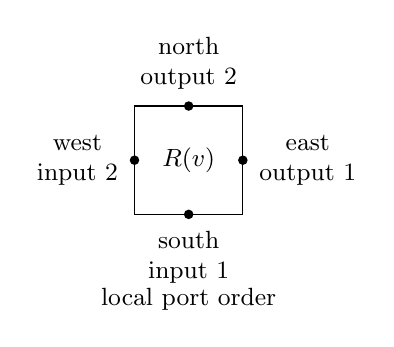
\begin{tikzpicture}[scale=.86,every node/.style={font=\small}]
 \draw (-.8,-.8) rectangle (.8,.8);
 \node at (0,0) {$R(v)$};
 \foreach \x/\y in {0/-.8,-.8/0,.8/0,0/.8}
    \fill (\x,\y) circle (2pt);
 \node[below,align=center] at (0,-.9) {south\\input 1};
 \node[left,align=center] at (-.9,0) {west\\input 2};
 \node[right,align=center] at (.9,0) {east\\output 1};
 \node[above,align=center] at (0,.9) {north\\output 2};
 \node at (0,-2.05) {local port order};
\end{tikzpicture}
\hspace{1cm}
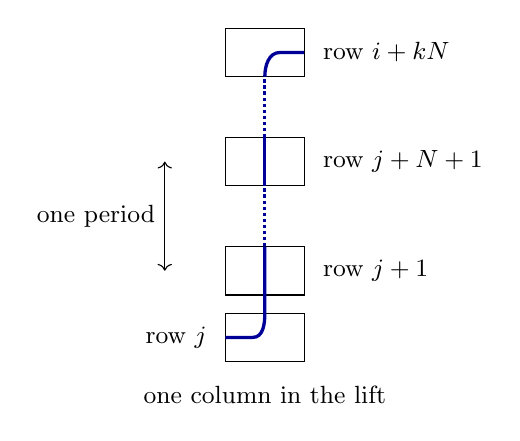
\begin{tikzpicture}[scale=.77,every node/.style={font=\small}]
 \foreach \y in {0,1.1,2.9,4.7}
    \draw (-.65,\y-.4) rectangle (.65,\y+.4);
 \draw[very thick,blue!60!black] (-.65,0) -- (-.2,0)
     to[out=0,in=-90] (0,.4) -- (0,1.5);
 \draw[very thick,blue!60!black,densely dotted] (0,1.5) -- (0,2.5);
 \draw[very thick,blue!60!black] (0,2.5) -- (0,3.3);
 \draw[very thick,blue!60!black,densely dotted] (0,3.3) -- (0,4.3);
 \draw[very thick,blue!60!black] (0,4.3)
     to[out=90,in=180] (.25,4.7) -- (.65,4.7);
 \node[left] at (-.8,0) {row $j$};
 \node[right] at (.8,1.1) {row $j+1$};
 \node[right] at (.8,2.9) {row $j+N+1$};
 \node[right] at (.8,4.7) {row $i+kN$};
 \draw[<->] (-1.65,1.1) -- (-1.65,2.9)
     node[midway,left] {one period};
 \node[below,align=center] at (0,-.65) {one column in the lift};
\end{tikzpicture}
\caption{The boxes show cyclic port order, rather than physical angles.
On the right, dotted portions contain the omitted intermediate rhombi.
The two displayed south--north passages are one period apart, so they
visit the same vertices after projection onto the cylinder. In the
planar lift all rhombi used are distinct.}
\label{fig:E-local-connector}
\end{figure}

Concatenate lifts of bridges counted by the divergent entry with
copies of this connector, always in successive disjoint column slabs.
Their interiors are disjoint, so the resulting planar path is
self-avoiding. To recover the concatenation, list all column cuts
that the path meets exactly once. Between two adjacent column cuts
in this list, a width-one subbridge inside any original valid slab
is still projection-valid. The inserted connectors are precisely the
projection-invalid width-one subbridges: they occupy one entire
column and their two cuts are crossed only at their endpoints.
Thus the connectors, the intervening slabs, and their original paths
are uniquely recovered from the concatenated path.

Choose finitely many valid slab widths whose total mass is $B$ with
$aB>1$. The width generating function of one valid-slab--connector
block is $g(z)=a\sum_M b_M(i,j)z^{M+1}$, with the sum restricted to
those widths. It satisfies $g(0)=0$ and $g(1)>1$. Hence the generating
function $\sum_{r\ge0}g(z)^r$ of recoverable concatenations has radius
strictly less than one. Each slab has at most a fixed constant times
its width in vertices, because its projection is self-avoiding on a
fixed cylinder; the connector has bounded length. Consequently all
these planar paths of total width $w$ have length at most $C_Nw$.
Their total critical weight is bounded above by the sum of
$c_n\rho^n$ for $n\le C_Nw$, up to fixed endpoint factors. This is
$\exp(o(w))$ by Proposition~\ref{prop:02-critical}, contradicting the
radius just obtained.

\end{proof}

\begin{proposition}[Physical cylinder vacuum]
At physical row parameters $u_i\in\{\lambda,2\lambda\}$,
\label{prop:02-cylinder-vacuum}
the column $T(3\lambda)$ restricted to vectors with zero empty
component has spectral radius less than one. Its unique stationary
state with empty component one is the regular continuation of $U_N$.
It equals the absolutely convergent sum of half-cylinder configurations
with vacant far boundary. The right-half state is
$U_N(3\lambda-u_1,\ldots,3\lambda-u_N)$.
\end{proposition}
\begin{proof}
A nonzero diagram propagated from a nonempty input pairing either
has a west-to-east spanning path or closes a discarded cycle. The
number of path segments is bounded at fixed $N$. Discarding their
mutual avoidance bounds their weights by a product of an exponentially
decaying spanning sum from Lemma~\ref{lem:02-periodic-slab} and
subexponential same-side sums. Therefore
the transfer on the subspace of zero empty component has spectral
radius strictly below one. The empty component itself is invariant.
Writing the transfer in these two blocks proves uniqueness and local
analyticity of its normalized fixed vector, and convergence from a
vacant far boundary proves the half-cylinder interpretation.
The rational stationary vector $V_N/h_N$ agrees with it wherever
defined nearby, hence extends to the physical parameters. Horizontal
reflection gives the stated right-half arguments. Vertical reflection
also recovers the covariance proved algebraically above.
\end{proof}

\subsection{The finite separating-loop formula}

Split the cyclic list into consecutive groups $X,Y$ of sizes $s,b$,
where $N=s+b$, and mark the two seams. Define $Z_{X,Y}(\chi)$ by
contracting the left and right vacuum states, assigning a closed loop
weight $\chi$ if it crosses the $X$ portion of the cut an odd number
of times, and weight zero otherwise. The empty configuration contributes
one. If a group is empty all loops have weight zero, so $Z=1$.
At physical parameters the markers are face centers. Compactifying
the cylinder ends gives a sphere, on which the odd-intersection rule
is precisely separation of the markers. Therefore $Z_{X,Y}(\chi)$
counts disjoint polygon families all separating the markers, with
weight $\prod_\ell\chi\rho^{|\ell|}$. Every such loop meets the cut;
disk connectivity on its two sides suffices to test separation.
The half-cylinder sums converge absolutely, and a family has a
bounded number of loops at fixed $N$, so this interpretation is valid
for every fixed $\chi$.

For the balanced observable $Z_N$ of the introduction, $N=2m$ and
the prescribed row list is $m$ copies of $2\lambda$ followed by $m$
copies of $\lambda$. Identify the triangular lattice with the complex
plane and start its column cut at the face center $f_1=0$. Its successive
edges have these row vectors, so the second marker and period are
\[
 f_2=m e^{2\pi i/3}=-\frac N4+i\frac{N\sqrt3}{4},\qquad
 V=m(e^{2\pi i/3}+e^{\pi i/3})=i\frac{N\sqrt3}{2}.
\]
The two groups are the two portions of this prescribed cut from $0$
to $f_2$ and from $f_2$ to $V$. Translation or reflection gives the
same observable. In particular the markers are half a period apart in
height; their longitudinal displacement is fixed by this construction.

\begin{lemma}[Characterization of the contraction]\label{lem:02-characterization}
The rational functions $Z_{X,Y}(\chi)$ are uniquely determined by the
following properties, with $\chi$ fixed.
\begin{enumerate}
\item $H_{X,Y}=h_N(X,Y)^2Z_{X,Y}$ is polynomial of degree at most
$2N-2$ in each argument, and $Z$ is symmetric within each group.
\item An ascending merge or deletion within either group leaves $Z$
unchanged after making the corresponding replacement or deletion.
\item Sending one argument to zero or infinity omits that site.
\item Sending $x\in X$ and $y\in Y$ to infinity at fixed generic
ratio gives
\[
 Z_{X,Y}\longrightarrow Z_{\widehat X,\widehat Y}Z_{x,y},
 \qquad Z_{x,y}=1+\chi(2c)^2\frac{xy}{(x+y)^2}.
\]
\item At size zero, $Z=1$.
\end{enumerate}
All limits are rational limits at generic values of the remaining
arguments. Hats mean omission of the indicated sites.
\end{lemma}
\begin{proof}
The right-half arguments are $q^3/x_i$. Equation~\eqref{eq:02-reciprocity},
homogeneity, and the per-slot degree bounds for $V_N$ give the
polynomial bound for $H$: occupied half-powers occur in pairs in the
contraction. To exchange sites within a group, move a symmetric braid
box from one side of the contraction to the other by transposition.
The two states braid in opposite directions because the starred
arguments reverse differences. Loop parity is preserved: following
the arcs in the box layer shows that each resulting loop has an even
total number of $X$-hits on the two interfaces of that layer. Thus
any cycle discarded on one side has zero gluing weight as well.
This proves symmetry and also permits a same-group splitting layer
to be moved through the contraction. At the descending specialization
on the starred side, apply $R(j\lambda)=S_jS_j^{\mathsf t}$ and the
ascending splitting identity. To cancel $S_j$, project its output onto diagrams whose first new
slot is vacant. For $S_2$, omitting that slot leaves the diagonal map
with coefficients $1$ on a vacancy and $\rho$ on an occupied strand.
For $S_3$, both new slots are then vacant; omitting them gives the
identity. Thus $S_j$ is injective, and
$S_jU_{\rm red}=S_jS_j^{\mathsf t}U_{\rm desc}$ implies
$S_j^{\mathsf t}U_{\rm desc}=U_{\rm red}$. This proves
the reduction of $Z$.

Cyclic covariance and the last-slot leading coefficient show that
sending one argument to infinity inserts a vacant site in the left
vacuum. Reflection gives the same statement in the right vacuum.
Horizontal reflection gives the limit at zero.

For completeness, the simultaneous two-site limit requires more than
the individual limits. Reorder within groups so that $x,y$ are adjacent
across a marker, and rotate them to the last two positions. Write
$P$ for the other $N-2$ arguments. We claim
\begin{equation}\label{eq:02-pair-limit}
 \frac{V_N(P,x,y)}{(xy)^{N-2}}
 =V_{N-2}(P)\otimes V_2(x,y)+o(|x|),
 \qquad
 V_2(x,y)=(x+y)\varnothing+2c\sqrt{xy}\,\mathrm{cup}.
\end{equation}
Fix square-root branches on the scaling ray. In the interpolation in
$y$, the deletion nodes are $y_z=q^3z$ for $z\in(P,x)$. For $N\ge3$,
nodes belonging to $P$ have data $O(|x|^{N-1})$, cardinal factors
$O(|x|^{N-3})$, and additional occupied square-root ratios at most
$O(|x|^{1/2})$. After division by $(xy)^{N-2}$ they are $o(|x|)$.
The leading vacant interpolation term becomes
$(y-y_x)V_{N-2}\otimes\varnothing+o(|x|)$. At $y_x=q^3x$ the data are
\[
 (x+y_x)\prod_{p\in P}(p-q^{-3}x)(p-q^6x)\,S_3V_{N-2}(P).
\]
The cardinal factor is asymptotic to $(y/y_x)^{N-2}$, with an extra
$\sqrt{y/y_x}$ on occupied output. Since $q^{-3}q^6=q^3$, these
terms give exactly the remaining terms in Equation~\eqref{eq:02-pair-limit}.
The expression for $V_2$ follows directly from the size-two
interpolation. Division by the empty components gives factorization
of the normalized left vacuum, and reflection gives that of the
right vacuum. The intersection-parity rule factors on the two
subsystems, proving both the pair limit and the displayed $Z_{x,y}$.

To prove uniqueness, the zero-site value and omission already settle
$N=1$. At $N=2$ with one site in each group, omission at zero and
infinity leaves only a possible difference $Cxy$ of the cleared
numerators. Its quotient by $h_2^2=(x+y)^2$ has a nonzero paired
scaling limit unless $C=0$, so the specified pair limit settles this
case. For all other group sizes, induct on $N$ and subtract two
candidate cleared polynomials. The known
scalar reductions of $h_N$ turn the reductions of $Z$ into identical
values of these polynomials at each split. Omission at zero kills
their constant coefficient, and
omission at infinity kills their leading coefficient. In a variable
of a group of size $s$, symmetry and the two reductions supply
$4(s-1)$ roots, namely $q^{\pm2}$ and $q^{\pm3}$ times every other
same-group argument. If $s>b$, these roots, together with the zero
constant coefficient, exceed the remaining degree $2N-3$.
If $s=b\ge2$, the difference must be a constant multiple of
\begin{equation}\label{eq:02-uniqueness-factor}
 \left(\prod_i x_i\right)
 \prod_{\substack{i<j\\\text{same group}}}
       (x_i^2+x_j^2)D_0(x_i,x_j).
\end{equation}
Indeed its degree in each variable is $1+4(s-1)=2N-3$, exactly the
remaining bound, so the quotient has degree zero in every variable.
When one argument from each group tends to infinity, this factor has
the same leading order as $h_N^2$ and a nonzero generic coefficient.
The pair limit forces the rational difference to tend to zero, so
its constant multiplier vanishes. The size-zero and size-two
conditions cover the remaining balanced cases.
\end{proof}

Using the fixed square roots, define the centered normalization
$\widetilde h_N=h_N\prod_i x_i^{-(N-1)/2}$. Its square is
\[
 \widetilde h_N^2=\frac{h_N^2}{\prod_{i<j}x_ix_j}
                 =\frac{h_N^2}{\prod_i x_i^{N-1}}.
\]
\paragraph{The three labels as formal site strings.}
Before writing the label sum, we construct its pair weights. Give a
site in group $\sigma=+1$ on $X$ or $\sigma=-1$ on $Y$ a generic
logarithmic coordinate $a_i$, with $x_i=e^{a_i}$. Here $a_i$ denotes
a logarithm, distinct from the earlier open-strip cosine coordinate.
Attach a formal string of length $a\in\{0,1,2\}$ at
\[
 a_i+i\sigma\beta,\ldots,a_i+i\sigma a\beta,
 \qquad l=\sigma(1-a).
\]
These are prescribed spectral points, with no integration variables
yet; at length zero the string is empty. Thus the three labels record
the three possible string lengths.
At this stage we assign weights only between distinct site strings;
factors within one string, which have poles at these spectral points,
will later be evaluated by residues.
We will first verify the resulting finite algebraic formula, and then
realize these strings as residues of a particle integral.

Put $P_j(r)=-2\sinh((r+ij\beta)/2)$. Products below are evaluated
at the coordinate difference of their arguments. For two objects
in the same group, the site--site, particle--site, and
particle--particle factors are, respectively,
\begin{equation}\label{eq:02-same-factors}
 B_s=P_2P_{-2}P_3P_{-3},\qquad
 F_s=(P_1P_{-1})^{-1},\qquad
 E_s=P_0^2P_2P_{-2}F_s.
\end{equation}
For different groups always use the plus coordinate minus the minus
coordinate, and use
\begin{equation}\label{eq:02-cross-factors}
 B_c=P_2^2P_3^2,\qquad F_c=P_1^{-2},\qquad E_c=P_0^2P_2^2F_c.
\end{equation}
The same-group factors are even, so no ordering convention is needed
there.

For ordered groups $\sigma,\omega$ and site labels $l,k$, let
$a=1-\sigma l$ and $b'=1-\omega k$, with the plus group first
when they differ. Let $z$ be the difference of the two site coordinates.
Multiply their site--site factor, all factors from a particle in either
string to the other site, and all factors between particles in different
strings. Denote this mutual product by
$\mathcal S^{\sigma\omega}_{lk}(z)=\prod_jP_j(z)^{n_j}$.
No factor internal to either string occurs. The exponents are encoded by
the Laurent polynomial
\begin{equation}\label{eq:02-string-polynomial}
 \sum_j n_j\xi^j=B-F(A+D)+EAD,\qquad
 A=\sum_{h=1}^a\xi^{\sigma h},\qquad
 D=\sum_{h=1}^{b'}\xi^{-\omega h}.
\end{equation}
Here, for $\sigma=\omega$,
\[
 B=\xi^2+\xi^{-2}+\xi^3+\xi^{-3},\quad F=\xi+\xi^{-1},\quad
 E=2+\xi^2+\xi^{-2}-F;
\]
for $\sigma=1,\omega=-1$,
\[
 B=2\xi^2+2\xi^3,\qquad F=2\xi,\qquad E=2+2\xi^2-F.
\]
Labels $l,r$ belong to $\{1,0,-1\}$, also denoted $+,0,-$, and
$v_l=2+l^2$. For a pair of sites set $e=1$ if they belong to the
same group and $e=-1$ otherwise. The arrays below are indexed by
$j\in\Z/8\Z$. A bracket $[a,b,\ldots]$ denotes the sum of the
corresponding unit vectors; repeated entries are counted with their
multiplicity. Rows and columns are ordered $+,0,-$; a matrix entry $0$ is the zero
vector, whereas an entry $[0]$ is the unit vector at residue zero:
\begin{equation}\label{eq:02-m-arrays}
\begin{split}
 m^+&=\begin{pmatrix}
 [2,3,5,6]&[3,5,6]-[0]&[5,6]-[0,1]\\
 [2,3,5]-[0]&[2,3,5,6]-[1,7]&[3,5,6]-[0]\\
 [2,3]-[0,7]&[2,3,5]-[0]&[2,3,5,6]
 \end{pmatrix},\\
 m^-&=2\begin{pmatrix}
 0 &[5]&[5,6]\\
 [3]&[4]&[5]\\
 [2,3]&[3]&0
 \end{pmatrix}.
\end{split}
\end{equation}
Define
\begin{equation}\label{eq:02-Q}
 Q^e_{lr}(u)=q^{ev_lr}u^{-1-elr}
       \prod_{j=0}^7(1-uq^{-j})^{m^e_{lr}[j]}.
\end{equation}

Substitution of $a,b'\in\{0,1,2\}$ gives
$\sum_{j\equiv-h\ (8)}n_j=m^{\sigma\omega}_{lk}[h]$.
Since
\[
 P_j(z)=e^{-(z+ij\beta)/2}(1-e^zq^j),
\]
the ratio of $Q^{\sigma\omega}_{lk}(e^z)$ to the string product is
$q^{\sigma\omega v_lk+\sum_j jn_j/2}$.
Differentiating Equation~\eqref{eq:02-string-polynomial} at $\xi=1$
gives the pair-phase identity
\begin{equation}\label{eq:02-string-phase}
 \frac{Q^{\sigma\omega}_{lk}(e^z)}{\mathcal S^{\sigma\omega}_{lk}(z)}
 =q^{\sigma\omega(v_lk+v_kl)/2}
 \begin{cases}
 1,&\sigma=\omega,\\
 (-1)^{1-lk},&\sigma=1,\ \omega=-1.
 \end{cases}
\end{equation}


\begin{theorem}[Finite cylinder formula]\label{thm:02-finite-formula}\label{E:finite-cylinder}
For $\chi=q^{-3}\tau+q^3\tau^{-1}$ and $\tau\ne0$,
\begin{equation}\label{eq:02-finite-formula}
 \widetilde h_N^2Z_{X,Y}(\chi)
 =\sum_{\substack{l_i\in\{-1,0,1\}\\
           \sum_{i\in X}l_i=\sum_{i\in Y}l_i=M}}
       \tau^M(-2c)^{\sum_i l_i^2}
       \prod_{i<j}Q^{e(i,j)}_{l_il_j}(x_i/x_j).
\end{equation}
The sum includes all allowed integers $M$. Apparent singularities at
colliding arguments are evaluated by continuation.
\end{theorem}
\begin{proof}
We verify the characterization in Lemma~\ref{lem:02-characterization}.
The arrays satisfy
\[
 \sum_jm^e_{lr}[j]=2+2elr,\qquad
 \sum_jj\,m^e_{lr}[j]\equiv e(v_lr-v_rl)\pmod8,
\]
and their exponents reverse under transposition. These identities give
$Q^e_{lr}(u)=Q^e_{rl}(1/u)$ and hence within-group symmetry.
The only possible finite nonzero poles are same-group poles at
$u=1,q,q^{-1}$. At $u=1$ only unequal labels are singular, with simple
poles, and exchanging these labels cancels the residues. At $u=q$
the singular labels are $(+,-)$ and $(0,0)$. The first kernel divided
by the second tends to $-1/(4c^2)$; the ratio of the corresponding
spectator products for a spectator of label $k$ and relative type
$e$ is $q^{ek}$. Neutrality makes the product of these spectator
ratios one. The site weight ratio is $4c^2$, so the residues cancel.
Reciprocity treats $q^{-1}$. Cross-group kernels have no such poles.

Here are the finite calculations that also verify the reductions.
For a same-group pair $x,y$, put $u=x/y$ and $w=qy$:
\[
\begin{array}{c|c|c}
 u&(l,r)&\text{nonzero value or pole coefficient}\\\hline
 q\ \text{(pole)} &(+,-),(0,0)&-i(2+2\sqrt2),\quad 2i\sqrt2\\
 q^2 &(+,0),(+,-),(0,-)&2q,\quad(2c^2)^{-1},\quad2q^{-1}\\
 q^3 &(+,-)&1
\end{array}
\]
In the first row the entries mean pole coefficients, obtained after
multiplication by $1-u/q$. At $q^2$, set
$L=l+r$ and $J=v_l+v_r-v_L-l+r$; the three surviving cases have
$J=1,2,1$. Their spectator ratios are
\[
 \frac{Q^e_{lk}(x/z)Q^e_{rk}(y/z)}{Q^e_{Lk}(w/z)}
       =q^{eJk}\frac{(w+z)^2}{wz}.
\]
At $q^3$ the product of spectator factors is
\[
 Q^e_{+k}(x/z)Q^e_{-k}(y/z)
 =q^{3ek}\frac{(z-q^{-3}y)^2(z-q^6y)^2}{xyz^2}.
\]
These identities require only the following identities of the
exponent arrays, with indices taken modulo eight:
\[
\begin{split}
 m^e_{+k}[j+1]+m^e_{-k}[j]
     &=m^e_{0k}[j+1]+m^e_{0k}[j],\\
 m^e_{lk}[j+1]+m^e_{rk}[j-1]-m^e_{Lk}[j]
     &=2\delta_{j,4}\qquad(u=q^2),\\
 m^e_{+k}[j+3]+m^e_{-k}[j]
     &=2\delta_{j,2}+2\delta_{j,3}\qquad(u=q^3).
\end{split}
\]
The constants follow from
$1-q^a=-2ie^{ia\beta/2}\sin(a\beta/2)$.
For the spectators, neutrality gives $\sum ek=-(l+r)$.
Including site weights, the $q^2$ reduction is therefore multiplication
by
\[
 2\prod_z\frac{(w+z)^2}{wz},
\]
and the $q^3$ reduction is multiplication by
\[
 (2c)^2\prod_z\frac{(z-q^{-3}y)^2(z-q^6y)^2}{xyz^2}.
\]
These are precisely the homogeneous scalar quotient rules for
$\widetilde h_N^2$; division verifies the two reductions of $Z$.

For a single argument $x$ with label $l$, reciprocity and neutrality
bound the product of its interactions by order $x^{N-1-l^2}$ at
infinity and $x^{-(N-1)+l^2}$ at zero. Only $l=0$ contributes at
leading order. Its phases multiply to one, leaving respectively
$\prod_zx/z$ and $\prod_zz/x$, exactly the leading factors of
$\widetilde h_N^2$. Pole cancellation and these bounds also prove
the required polynomial degree after removing the centering.

For $x\in X,y\in Y$ tending to infinity together, interactions with
the remaining arguments have order
$|x|^{2(N-2)-(l-r)^2}$. Only $l=r$ survives at leading order.
Neutrality cancels the phases and ratio powers, leaving
$\prod_zxy/z^2$ times the separate pair and remaining expressions.
This agrees with Equation~\eqref{eq:02-pair-limit} for the scalar
normalization. Finally, the two-site sum over the three equal labels
is
\[
 \frac{(x+y)^2}{xy}+\chi(2c)^2,
\]
and the zero-site sum is one. Lemma~\ref{lem:02-characterization}
now proves the formula.
\end{proof}

\subsection{Contour sectors and residue cancellation}

For the asymptotic application, $s=b=m$, $N=2m$, and the arguments
in $X,Y$ will be respectively $1,q^{-1}$. These are obtained from the
physical row parameters $2\lambda$ on $X$ and $\lambda$ on $Y$, whose
$x$-values are $q^2,q$, by the common rescaling $x_i\mapsto q^{-2}x_i$.
Homogeneity of $V_N$ and $h_N$ leaves their quotient and the contraction
unchanged. We first keep the two rays apart and allow distinct real
offsets. Denote the groups by
$\sigma=+1,-1$, in that order, and set
\[
 \alpha_+=0,\qquad \alpha_-=-\varepsilon\beta,\qquad
 0<\varepsilon<1.
\]
Specialize the logarithmic site coordinates to
$\Im a_i=\alpha_{\sigma_i}$. Eventually $\varepsilon=1$ and the real offsets coalesce to zero.

A particle of group $\sigma$ at shift $j$ has coordinate
$u+i\alpha_\sigma+i\sigma j\beta$, with $u\in\R$ and measure
$du/(2\pi)$. There are three species in each group:
\[
\begin{array}{c|c|c}
 \text{species}&\text{shifts of its elementary particles}&\text{activity}\\\hline
 \text{main singleton}&0&p_\sigma\\
 \text{far singleton}&11/4&-p_\sigma\\
 \text{far double}&5/2,\ 7/2&4c^2p_\sigma^2
\end{array}
\]
The signed far species make the residue representation exact. When the
main contours are moved outward, particles left on the far contour
cancel against the negative far singletons; a particle attaching to
one of those singletons cancels an original far double. The surviving
configurations will therefore be strings of zero, one, or two particles
attached to each site. The proof below establishes this cancellation
with the factorials and phases retained.

The two constituents of a double share one real variable. For fixed
numbers $n_\sigma,t_\sigma,D_\sigma$ of the three species, multiply
all site--site factors, all particle--site factors, and all
particle--particle factors between elementary constituents, omitting
the internal $E_s$ between the two constituents of a single double.
Integrate over the real variable of every singleton and double.
Multiply the integral by
\[
 \prod_{\sigma=\pm1}
 \frac{p_\sigma^{n_\sigma}(-p_\sigma)^{t_\sigma}
                   (4c^2p_\sigma^2)^{D_\sigma}}
      {n_\sigma!\,t_\sigma!\,D_\sigma!}.
\]
Let $I$ denote the sum of these terms through total elementary degree
$\sum_\sigma(n_\sigma+t_\sigma+2D_\sigma)\le N$. This finite
truncation is sufficient for every coefficient used below; no
convergence assertion for an infinite activity series is needed.

\begin{theorem}[Contour-sector representation]\label{thm:02-contour-sectors}\label{E:contour-sectors}
For the prescribed site rays, every $0<\varepsilon<1$, and every
$\eta\in\mathbb C$, put $\chi=2\cos\eta$. Then
\begin{equation}\label{eq:02-contour-sectors}
 \widetilde h_N^2Z_{X,Y}(2\cos\eta)
 =(2d)^N\sum_{M=-\min(s,b)}^{\min(s,b)}
       (-1)^{sb+M}e^{i\eta M}
       [p_+^{s-M}p_-^{b+M}]I.
\end{equation}
The coefficient integrals are absolutely convergent. The identity
extends to $\varepsilon=1$ and to coincident real site offsets by
continuation and dominated convergence of the fused integrands.
\end{theorem}
\begin{proof}
\emph{Integrability and contour geometry.}
All coefficient terms on the right have exactly $N$ elementary
particles, because $(s-M)+(b+M)=N$. A particle at real coordinate $u$ receives decay
$O(e^{-N|u|})$ from the $N$ sites; a pair interaction grows at most
$O(e^{|u-u'|})$. The inequality
$|u-u'|\le|u|+|u'|$ therefore bounds the full integrand away from
its prescribed poles by a constant times
$\exp(-\sum|u|)$, counting elementary coordinates with multiplicity.
The same estimate applies to smaller elementary degree and to
fused particles or residues. Constants may depend on $N$, sites,
and the fixed contours. This proves the convergence needed for
contour movements and removal of their vertical ends.

For $\varepsilon<1$, temporarily move the far singletons to a common
shift $h$ and the far doubles to $h-1,h$, where
\[
 3<h<\frac{7-\varepsilon}{2}.
\]
The offsets are measured outward from each group's site ray, in units
of $i\sigma\beta$:
\[
\begin{array}{c|c|c}
 &\text{fixed offsets}&\text{temporary offsets}\\\hline
 \text{main singleton}&0&0\ \longrightarrow\ h\\
 \text{far singleton}&11/4&h\\
 \text{far double}&(5/2,7/2)&(h-1,h)\\
 \text{site residues}&\text{none initially}&1\ \text{or}\ (1,2).
\end{array}
\]
A parenthesized pair shares one real coordinate. Only the far contours
are moved in this first step; the main-contour arrow is the subsequent
deformation. Moving the far contours crosses no pole. Indeed the interaction of a double with any
particle has no poles after its two constituents are multiplied.
Relative to the double midpoint, the same-group fused $E_sE_s$
has only positive exponents at shifts $\pm1/2,\pm5/2$; the cross-group
product has exponent two at $-1/2,5/2$. The same observation applies
to pairs of doubles. Far particle--site poles are avoided because
all far constituent shifts stay in $(2,7/2]$. For opposite-group
singletons the cross difference lies strictly between zero and seven
in shift units.

\emph{Residues and cancellation of unbound particles.}
Move the main contours from shift zero to shift $h$. A same-group
site can collect an ordered string of length $a=0,1,2$, at its own
coordinate plus $i\sigma\beta,\ldots,i\sigma a\beta$.
The first attachment occurs at shift one; interaction with it permits
a second at shift two. An attempted third at shift three is canceled
by the zero in its interaction with the first. Quadratic coincidence
zeros likewise cancel attempts to attach twice at the same root.
A main particle can also attach one unit below an original far
singleton, converting it into a double. These are all possibilities:
fused doubles have no particle poles, and $2h+\varepsilon<7$
excludes cross-group poles.

Here is an ordering of the deformation that avoids any ambiguity
from moving poles. Divide $[0,h]$ into generic layers of thickness
less than $1/3$, separating the levels $2$ and $h-1$. In each layer
move the remaining unbound variables one at a time; freeze every
picked residue immediately, including during the rest of that layer.
Unbound variables in a common group then never differ by a full unit
of shift, so they do not create poles with one another. For fixed
generic distinct real coordinates of original far particles, also
distinct from site offsets, these are ordinary one-variable contour
moves across simple poles. An attached far spectator appears as the
complete double interaction. An unconverted far singleton is more
than one shift unit beyond every site-bound root. Thus residual
integrands have no unaccounted coincident-spectator singularity and
satisfy the preceding decay bound. The identities can consequently
be integrated over the original far spectators as well.

The internal weight of a string, including its factors with its own
site and excluding activities, is
\begin{equation}\label{eq:02-string-residues}
 r_0=1,\qquad r_1=\frac1{2d},\qquad r_2=\frac{c^2}{d^2}.
\end{equation}
With measure $du/(2\pi)$, the oriented residue multiplier is
$i\sigma$. The first $F_s$ pole contributes $1/(2d)$. The second
attachment contributes $-4c^2$ from the $E_s$ pole at relative
$i\sigma\beta$, and $F_s(2i\sigma\beta)=-1/(2d)$ from its
site factor. Multiplication gives $r_2$. Attachment at relative
$-i\sigma\beta$, below a far singleton, instead contributes
$4c^2$.

Fix a site-string pattern. The effective far singleton activity is
$-p_\sigma+p_\sigma=0$, from original and unpicked main singletons.
The effective far double activity is
$4c^2p_\sigma^2+4c^2(-p_\sigma)p_\sigma=0$, from original doubles
and attached original singletons. These cancellations respect all
factorials. Explicitly, start in one group with $n,t,D$ particles of
the three species. If $r$ main particles fill the specified site
strings and $a$ attach to $a$ of the original far targets, summing
labeled assignments leaves factorial coefficient
\[
 \frac1{(n-r-a)!\,(t-a)!\,a!\,D!}.
\]
Each assignment determines exactly one contour term through its
choices at shifts $1,2,h-1$. The remaining two kinds of singleton
and two kinds of double can therefore be combined by the binomial
formula. This argument is coefficientwise in $p_+,p_-$, so all
canceling terms have the same elementary total. Only completely
site-bound configurations survive. In particular every cancellation
used for the degree-$N$ coefficients takes place inside the finite
truncation defining $I$.

\emph{Identification with the finite label formula.}
Assign label $l=\sigma(1-a)$ to a site in group $\sigma$ with string
length $a$. The coefficient constraints become
$\sum_{X}l_i=\sum_{Y}l_i=M$. We check their mutual weights explicitly.
Use the formal string weights and their pair-phase identity
\eqref{eq:02-string-phase} established before the finite formula.
To multiply these phases without a size restriction, put
$\sigma_i=1$ on $X$, $\sigma_i=-1$ on $Y$, and $v_i=2+l_i^2$.
Neutrality gives $\sum_i\sigma_i l_i=0$, while $l_i^3=l_i$. Hence
\[
\begin{aligned}
\frac12\sum_{i<j}\sigma_i\sigma_j(v_i l_j+v_j l_i)
 &=\frac12\left[
    \left(\sum_i\sigma_i v_i\right)
    \left(\sum_i\sigma_i l_i\right)-\sum_i v_i l_i\right]\\
 &=-\frac32\sum_i l_i=-3M.
\end{aligned}
\]
The cross sign is
$(-1)^{sb-(\sum_Xl_i)(\sum_Yl_i)}=(-1)^{sb-M^2}=(-1)^{sb+M}$.
Thus the product of all pair phases is exactly
$q^{-3M}(-1)^{sb+M}$. Finally, since $\sum_i a_i^{\mathrm{len}}=N$
for the string lengths $a_i^{\mathrm{len}}$,
\[
 (2d)^N\prod_i r_{a_i^{\mathrm{len}}}=(-2c)^{\sum_i l_i^2}.
\]
Indeed the per-site ratio of the right-hand weight to
$(2d)^a r_a$ is $(-2c)^{1-a}$, whose product is one.
Taking $\tau=q^3e^{i\eta}$ in Theorem~\ref{thm:02-finite-formula}
now proves Equation~\eqref{eq:02-contour-sectors}.

\emph{Confluent physical limits.}
Return the far contours to the fixed shifts in the definition of
$I$. Their fused pair products have no pole at $\varepsilon=1$.
On these fixed contours the same decay bound persists in a
neighborhood of that value and of confluent real site offsets.
This justifies both final limits.
\end{proof}

\begin{lemma}[Signs at the confluent rays]\label{lem:02-sector-signs}
At $\varepsilon=1$ with confluent real site offsets, extract constant
signs from the site factors and from each full pair of integration
variables, multiplying double constituents before doing so, so that
the value at zero real difference is positive, or its leading
quadratic coefficient is positive when it vanishes. Their logarithms
then satisfy conjugation under $u\mapsto-u$. They are regular on
$\R$ except for same-species coincidences with singular part
$2\log|u-u'|$, including double--double coincidences.
At fixed far counts, multiply the extracted signs by the explicit
prefactor $(-1)^{sb+M}$ in Equation~\eqref{eq:02-contour-sectors}.
The resulting sign has $M$-dependence exactly $(-1)^{fM}$, up to an
$M$-independent sign, where $f=f_X+f_Y$ is the number of far elementary
particles. The remaining explicit phase is $e^{i\eta M}$.
\end{lemma}
\begin{proof}
For real $r$, $P_j(-r)=-\overline{P_j(r)}$. Each fused product has
even total exponent, which gives the asserted conjugation after a
real sign has been extracted. Real zeros of an elementary factor occur
only at $r=0$ and $j\in8\mathbb Z$. Combine the exponents before
testing for a zero, in particular for the two constituents of a
double. Ordered by main singleton, far singleton, and far double,
the extracted pair signs and vanishing orders are
\[
\begin{array}{c|c|c}
 &\text{sign matrix}&\text{order matrix at }r=0\\\hline\noalign{\vskip 3pt}
\text{same group}&
 \begin{pmatrix}+&-&+\\-&+&+\\+&+&+\end{pmatrix}&2I_3\\\noalign{\vskip 3pt}
\text{different groups}&
 \begin{pmatrix}-&-&+\\-&-&+\\+&+&+\end{pmatrix}&0.
\end{array}
\]
The site--particle signs are $(+,-,+)$ in the same group and
$(-,-,+)$ in different groups, with zero vanishing order in both
cases. These tables follow directly from $P_j(0)=-2i\sin(j\beta/2)$
and $P_{8k}(r)=-(-1)^kr+O(r^3)$: shift the exponents of
$P_0^2P_2P_{-2}/(P_1P_{-1})$ or $P_0^2P_2^2/P_1^2$ by every
constituent difference, add them, and cancel opposite powers. Thus
there are no other real singularities.

Let $n_\sigma,t_\sigma,D_\sigma$ count main singletons, far
singletons, and far doubles. Their elementary totals are
$K_+=s-M$ and $K_-=b+M$, with
$K_\sigma=n_\sigma+t_\sigma+2D_\sigma$.
The cross-group site and pair signs in the table have parity
\[
 bK_++sK_-+K_+K_-\equiv sb+M\pmod2.
\]
This cancels the prefactor in Equation~\eqref{eq:02-contour-sectors}.
The remaining negative factors are a same-group main--far-single
pair, a same-group far-single--site pair, and each far-single activity.
Their total parity is
\[
 (n_++s+1)t_++(n_-+b+1)t_-
 \equiv M(t_++t_-)\equiv Mf\pmod2,
\]
because $t_\sigma^2\equiv t_\sigma$ and
$f=t_++t_-+2D_++2D_-$. Doubles contribute only positive signs in
the tables. Any fixed extraction of the site--site signs is independent
of $M$. This proves the required imbalance phase.
\end{proof}

\subsection{The Pfaffian denominator at confluence}

The reference-kernel reduction uses Schur's Pfaffian identity and
Cauchy's determinant identity; see
\cite[equations (1.1)--(1.2)]{IshikawaOkadaTagawaZeng2006}.
We include their elementary forms in the present normalization.
The confluent kernel and its determinant asymptotic then require
the operator estimates below. This is an estimate for equal group
sizes. The contour identity above holds for unequal sizes as well,
but the present denominator theorem does not assert an asymptotic
uniform in that larger parameter domain.

In this subsection $N=2m$, the first $m$ logarithmic sites are zero,
and the last $m$ are $-i\beta$, all understood as confluent limits.
Set
\[
 \gamma=\frac43=\frac\pi{3\beta},\qquad
 L=\frac{\log N}{\gamma},\qquad
 H_*(u)=\frac{e^{2u}+2de^u+1}{(e^u-1)e^{u/2}}
                       \tanh\frac{\gamma u}{2}.
\]
At $u=0$ use the removable continuation of $H_*$.

\begin{theorem}[Balanced denominator asymptotic]\label{thm:02-denominator}\label{E:balanced-denominator}
For $N=2m\ge2$, with exactly $m$ sites at each of $0,-i\beta$, the
normalization $h_N$ is nonzero. As $N\to\infty$ through these even
sizes,
\begin{equation}\label{eq:02-denominator}
 \log\left|
 \frac{\widetilde h_N^2}
      {(\gamma/2)^N\prod_{i<j}H_*(a_i-a_j)^2}
 \right|
 =\frac5{24}\log N+o(\log N).
\end{equation}
\end{theorem}
\begin{proof}
First take distinct sites. Write
\[
 K(u)=\frac{\sinh u}{\cosh u+d},\qquad
 K_0(u)=\tanh\frac{\gamma u}{2}.
\]
Equation~\eqref{eq:02-h-pfaffian} and the definition of $H_*$ give
\begin{equation}\label{eq:02-determinant-ratio}
 \frac{\widetilde h_N^2}{\prod_{i<j}H_*(a_i-a_j)^2}
 =\frac{\det[K(a_i-a_j)]}{\det[K_0(a_i-a_j)]}.
\end{equation}
Here we used the Pfaffian identity
\[
 \operatorname{Pf}\left[\frac{v_i-v_j}{v_i+v_j}\right]
       =\prod_{i<j}\frac{v_i-v_j}{v_i+v_j},\qquad v_i=e^{\gamma a_i}.
\]
To prove it, clear denominators: the numerator is an alternating
polynomial of Vandermonde degree and is therefore a constant times
the Vandermonde. The residue at $v_{N-1}=-v_N$, followed by induction
from size two, determines the constant to be one.

For an even-dimensional skew matrix $A$, adding the all-ones matrix
does not change its determinant. Indeed the rank-one determinant
formula gives the extra term $\boldsymbol1^{\mathsf t}
\operatorname{adj}(A)\boldsymbol1$, which is zero since
$\operatorname{adj}(A)$ is skew. Apply this to both matrices in
Equation~\eqref{eq:02-determinant-ratio}, then conjugate by the
diagonal factors $e^{-\gamma a_i/2}$. The resulting reference kernel
is
\[
 G_0(u)=e^{-\gamma u/2}(1+K_0(u))
       =\operatorname{sech}(\gamma u/2),
\]
and the actual kernel is $G(u)=e^{-\gamma u/2}(1+K(u))$.
With Fourier convention $\widehat f(k)=\int_\R e^{-iku}f(u)\,du$
and $\zeta=\gamma/2+ik$, their transform ratio is
\begin{equation}\label{eq:02-fourier-ratio}
 \frac{\widehat G(k)}{\widehat G_0(k)}
 =\gamma\frac{\cos(\beta\zeta)\sin(\pi\zeta/\gamma)}
                    {\sin(\pi\zeta)}
 =\frac\gamma2(1+R(k)),\qquad
 R(k)=\frac1{2\cos(2\beta\zeta)}.
\end{equation}
For the first equality, put $t=e^u$ and use
\[
 1+K(u)=\frac{t}{t+e^{i\beta}}+\frac{t}{t+e^{-i\beta}},\qquad
 \int_0^\infty\frac{t^{p-1}}{1+t}\,dt=\frac\pi{\sin\pi p}.
\]
The beta integral follows by a keyhole contour, initially for
$0<\Re p<1$. The second equality in
Equation~\eqref{eq:02-fourier-ratio} follows from
$\pi/\gamma=3\beta$ and $\pi=4\beta$ by the triple-angle identity.

The determinant ratio is now explicit, but direct differentiation at
coalescing sites would obscure its size. We instead view the reference
matrix as a Gram matrix. Its orthogonal projection will occupy an
interval of length $2\gamma^{-1}\log N$ in the real direction; the
trace density on that interval will give the required logarithmic term.

We turn the determinant ratio into a finite-dimensional compression.
Let $\mathcal H$ be the Hilbert space with norm
\[
 \|f\|_{\mathcal H}^2
 =\int_\R|\widehat f(k)|^2v(k)\,\frac{dk}{2\pi},\qquad
 v(k)=\frac1{\widehat G_0(k)}
      =\frac\gamma{2\pi}\cosh\frac{\pi k}{\gamma}.
\]
Its functions have bounded evaluation at every
$z$ with $|\Im z|<\pi/(2\gamma)$. Write $k_z$ for the evaluation
vector, and $P=P_N$ for the orthogonal projection onto the span of
evaluations and their derivatives of orders $0,\ldots,m-1$ at
$z=\pm i\beta/2$. Centering the two site rays changes no differences. The derivative
evaluation vectors are linearly independent. Indeed, a linear relation
among them, written in Fourier variables and multiplied by the common
nonzero weight, has the form
$p_+(k)e^{\beta k/2}+p_-(k)e^{-\beta k/2}=0$ on $\mathbb R$, where
$p_+,p_-$ have degree at most $m-1$. Sending $k$ to $+\infty$ gives
$p_+=0$, and then $p_-=0$. Their Gram matrix is consequently positive
definite.

Start with distinct paired real offsets and permute columns by complex
conjugation; the reference matrix becomes the Gram matrix of these
evaluation vectors. The actual matrix represents the sesquilinear form with the
Fourier multiplier $\frac\gamma2(I+R)$ inserted. Passing to divided
differences gives the derivative vectors at confluence. Hence
\begin{equation}\label{eq:02-compression-determinant}
 \frac{\widetilde h_N^2}
 {(\gamma/2)^N\prod_{i<j}H_*(a_i-a_j)^2}
 =\det\left(I+PRP\big|_{\operatorname{ran}P}\right).
\end{equation}
The same column permutation is used in numerator and denominator,
so it introduces no sign in their ratio. The reference Gram matrix is
nondegenerate by the preceding independence argument.
Moreover $\operatorname{Re}R(k)\ge0$ for real $k$: since
$2\beta\operatorname{Re}\zeta=\pi/3$, the real part of
$\cos(2\beta\zeta)$ is $\tfrac12\cosh(2\beta k)>0$.
Thus $I+PRP$ is strictly accretive and invertible. Since the removable
factors $H_*(0)$ and $H_*(i\beta)$ are nonzero, the compression identity
already proves $h_N\ne0$ at these balanced confluent sites. The rest
of the proof determines its logarithmic size.

The projection has a useful exact localization formula:
\begin{equation}\label{eq:02-projection-complement}
 \|(I-P)k_z\|^2=\|k_z\|^2
 \prod_{\pm}
 \left|\frac{e^{\gamma z}-e^{\pm i\gamma\beta/2}}
 {e^{\gamma z}+\overline{e^{\pm i\gamma\beta/2}}}\right|^{2m}.
\end{equation}
To see this, augment the reference Gram matrix by $k_z$ and take its
Schur complement. Under $w=e^{\gamma z}$, its kernel is
$1/(w+\overline{w'})$ up to separate one-point factors. The Cauchy
determinant formula follows by clearing denominators and using
antisymmetry, with the constant fixed by residues. Its ratio after
augmentation is exactly Equation~\eqref{eq:02-projection-complement}.
Divided differences give its confluent version and prove the
nondegeneracy of the derivative Gram matrix.

For each fixed horizontal line in the evaluation strip, this implies
\begin{equation}\label{eq:02-projection-bound}
 \|Pk_z\|^2\le C\min\{1,Ne^{-\gamma|\Re z|}\}.
\end{equation}
Indeed, for $a=e^{\pm i\gamma\beta/2}$ and $w=e^{\gamma z}$,
\[
 1-\frac{|w-a|^2}{|w+\overline a|^2}
 =\frac{4\Re w\Re a}{|w+\overline a|^2}
 \asymp e^{-\gamma|\Re z|}.
\]
The product in Equation~\eqref{eq:02-projection-complement} is
therefore within $CNe^{-\gamma|\Re z|}$ of one, and is at most
$\exp(-cNe^{-\gamma|\Re z|})$. In particular, translated to the
frame of any real $x$ with $|x|\le(1-\delta)L$, the projections
$P_N$ converge strongly to the identity, uniformly for fixed
$\delta>0$. The complement tends uniformly to zero on every fixed
evaluation vector, and these vectors span a dense subspace by Fourier
uniqueness; contraction of the projections extends this to all of
$\mathcal H$.

Integrating Equation~\eqref{eq:02-projection-bound} on horizontal
lines near the two edges of the evaluation strip gives, for every
fixed $\epsilon>0$,
\begin{equation}\label{eq:02-trace-envelope}
 \operatorname{Tr}(Pe^{-\epsilon|k|}P)\le C_\epsilon L.
\end{equation}
Here multipliers are written as functions of $k$. More explicitly,
Plancherel on the line of height $y$ gives the multiplier
$v^{-1}e^{-2ky}$, and its trace against $P$ is
$\int_\R\|Pk_{x+iy}\|^2\,dx$. Choose $y$ near each strip edge.
The sum of the two resulting positive multipliers dominates a
constant multiple of $e^{-\epsilon|k|}$, while each integral is
$O(L)$ by Equation~\eqref{eq:02-projection-bound}.

We claim, for each integer $p\ge1$,
\begin{equation}\label{eq:02-trace-limit}
 \lim_{N\to\infty}\frac{\operatorname{Tr}((PRP)^p)}{2L}
       =\int_\R R(k)^p\,\frac{dk}{2\pi}.
\end{equation}
First truncate the exponentially decaying multiplier $R$ to a bounded
frequency interval. For any multiplier $H$,
\[
 \|PHP\|_1\le\operatorname{Tr}(P|H|P),
\]
by factoring through $|H|^{1/2}P$ and using the Hilbert--Schmidt
inequality. Equation~\eqref{eq:02-trace-envelope} makes the normalized
trace error tend to zero uniformly as the frequency interval grows;
a telescoping product gives the same statement for each fixed power.

For a bounded compactly supported symbol $S$, cyclicity of the trace
writes the corresponding trace as
\[
 \operatorname{Tr}\bigl(v^{-1}(Sv)P(SP)^{p-1}\bigr).
\]
The resolution
$\int_\R|k_x\rangle\langle k_x|\,dx=v^{-1}$ turns this trace into
$\int_\R F_N(x)\,dx$, where
\[
 F_N(x)=\left\langle(Sv)P(SP)^{p-1}k_x,k_x\right\rangle_{\mathcal H}.
\]
The real-line evaluation vectors have a fixed norm. The multiplier
$Sv$ is bounded on the compact frequency support, and the rightmost
operator acting on $k_x$ contains $P$. Hence
$|F_N(x)|\le C\|Pk_x\|$.
Translate $k_x$ to $k_0$ and conjugate every $P$ by the same real
translation. The multipliers are unchanged. In the bulk
$|x|\le(1-\delta)L$, strong convergence of these translated
projections therefore gives, uniformly,
\[
 F_N(x)\longrightarrow
 \left\langle S^pv k_0,k_0\right\rangle_{\mathcal H}
 =\int_\R S(k)^p\,\frac{dk}{2\pi}.
\]
The transition region has length $O(\delta L)$; beyond $(1+\delta)L$,
Equation~\eqref{eq:02-projection-bound} has an integrable exponential
tail of size $o(L)$. Divide by $2L$, then let $\delta\downarrow0$.
This proves the compact-frequency limit and hence
Equation~\eqref{eq:02-trace-limit}.

On the real frequency axis, $|R(k)|\le1$ and $\Re R(k)\ge0$:
here $2\beta\Re\zeta=\pi/3$. Moreover
$\|PRP\|_1=O(L)$ by Equation~\eqref{eq:02-trace-envelope}.
For $0<t<1$, the logarithmic power series and
Equation~\eqref{eq:02-trace-limit} yield
\[
 \lim_{N\to\infty}\frac1{2L}
       \operatorname{Tr}\log(I+tPRP)
 =\int_\R\log(1+tR(k))\,\frac{dk}{2\pi}.
\]
Accretivity gives $\|(I+tPRP)^{-1}\|\le1$ for $t\ge0$, so the
trace derivative is bounded by $\|PRP\|_1=O(L)$. The same integrable
bound holds for the limiting integral. Thus the limit extends to
$t=1$. Taking real parts is equivalent to taking the logarithm of
the determinant modulus in Equation~\eqref{eq:02-compression-determinant}.

Finally shift the contour from $\Re\zeta=\gamma/2$ to
$\Re\zeta=0$. The function
$\log(1+1/(2\cos(2\beta\zeta)))$ is analytic in the intervening
strip, with the branch tending to zero at imaginary infinity;
its horizontal-end contributions vanish exponentially. Therefore
\[
 \int_\R\log(1+R(k))\,dk
 =\int_\R\log\left(1+\frac1{2\cosh(2\beta k)}\right)\,dk
 =\frac{5\pi^2}{72\beta}.
\]
For the last evaluation use evenness and set $y=e^{-2\beta k}$ for
$k>0$. The logarithm becomes
$\log[(1-y^3)/((1-y)(1+y^2))]$. Termwise integration of its
convergent logarithmic series, or monotone limits of their integrals,
gives
\[
 \frac1\beta\int_0^1
 \frac{\log(1-y^3)-\log(1-y)-\log(1+y^2)}{y}\,dy
 =\frac1\beta\left(-\frac{\pi^2}{18}
                         +\frac{\pi^2}{6}-\frac{\pi^2}{24}\right)
 =\frac{5\pi^2}{72\beta}.
\]
Combining this with $2L/(2\pi)$ and
$\beta\gamma=\pi/3$ gives the coefficient
$5\pi/(72\beta\gamma)=5/24$ in
Equation~\eqref{eq:02-denominator}.
\end{proof}

\section{Centering, coercivity, and the fluctuation spectrum}\label{sec:03-gas-mean}

The finite contour formula expresses the cylinder partition function as
an oscillatory sum of particle integrals. We first identify its exact
mean density. Subtracting this density leaves an interaction whose real
part is positive and therefore controls both the particle counts and
excursions beyond a logarithmic wall. We then compare the interior
interaction with a reference ensemble whose normalization and linear
statistics can be evaluated. The energy estimates have two uses. The untruncated real energy estimate controls every valid particle count; the sharper imaginary trial fields identify the tilt cost in the fixed-fugacity exponent. Both use the same exact compensated-sector identity, Lemma~\ref{lem:03-compensated-sector}. The determinant asymptotic in Theorem~\ref{thm:03-determinant} supplies the remaining fluctuation contribution. Lemmas~\ref{lem:03-core} and~\ref{lem:03-schur} then give the finite-dimensional approximation needed to realize that determinant by moving actual particle coordinates.

\subsection{The exact mean density}

Throughout this section we specialize Theorem~\ref{thm:02-contour-sectors} to \(N=2m,\ s=b=m,\ \varepsilon=1\), all real site offsets zero. Fourier transforms in the real coordinate use \(e^{-iku}\) and inverse measure \(dk/(2\pi)\). A particle is specified by its real coordinate \(u\) and its ray label; the imaginary part of its logarithmic coordinate is determined by that label. An interaction matrix kernel acts by convolution; symmetric means \(H^{JI}(-u)=H^{IJ}(u)\), and forms with complex arguments are continued \emph{bilinearly}. Write
\[
 \gamma=\pi/(3\beta),\quad L=(\log N)/\gamma,\quad
 p=2\beta,\quad \kappa=(3\beta)^2 .
\]
Labels are \(I=(\sigma,J)\), where \(\sigma\in\{+1,-1\}\) and \(J=0,F,P\) denote the main, far-single and far-pair species. Their elementary shifts are, respectively, \(0\), \(11/4\), and \((5/2,7/2)\), as in Theorem~\ref{thm:02-contour-sectors}. Their multiplicities \(w_I\) are \(1,1,2\); a pair still has only one real integration variable. Write \(H\) for minus the sign-normalized particle-particle log interaction, \(V\) for the log (without negation) of the sign-normalized site-particle interaction (particle row, site column). Differences in these kernels take the first real coordinate minus the second, e.g. the exponentiated factors use \(H^{I I'}(u-u')\) with minus sign for labels \(I,I'\). More explicitly use linear combinations of
\[
 K_\theta(u)=-\log[2(\sin(\theta/2)\cosh(u/2)-i\cos(\theta/2)\sinh(u/2))],\qquad
 K_0(u)=-\log|2\sinh(u/2)|
\]
reducing angles to \([0,2\pi)\). Thus \(H\) uses the exponents of the log-sinh factors in \(E\) (fused for pair labels), and \(V\) the negative exponents in the site-particle product; cross terms in reverse order transpose and reflect the kernel. The exponents at angle zero in \(H\) are \(2\delta_{IJ}\) by the shift lists; there are no angle-zero terms of \(V\). These conventions agree with the sign normalization of the contour-sector identity.

Modulo distributions at zero frequency the transforms of \(K_\theta\) are
\[
 \pi e^{(\pi-\theta)k}/(k\sinh(\pi k)),\qquad
 \widehat K_0=\pi\cosh(\pi k)/(k\sinh(\pi k)).
\]
Indeed \(K_\theta''=\tfrac14/\sinh^2((u+i\theta)/2)\); shifting by a period and taking the double pole residue gives \(-\pi k e^{(\pi-\theta)k}/\sinh(\pi k)\). The second formula follows by even averaging as \(\theta\downarrow0\). Affine terms in comparisons below are fixed by tails: real parts \(-|u|/2+O(e^{-|u|})\), imaginary parts odd with limits given by \(\tfrac12(\pi-\theta)\operatorname{sign}u\) for \(0<\theta<2\pi\). For the main (near) labels,
\[
 \widehat H_{nn}(k)=\frac{2\pi c_*(k)}{k\sinh(\pi k)}
 \begin{pmatrix}\cosh(3\beta k)& e^{pk}\\ e^{-pk}&\cosh(3\beta k)\end{pmatrix},
 \qquad c_*(k)=2\cosh(\beta k)-1.
\]
Define \(\widehat\varrho=1/c_*\). Shifting by a period and taking simple residues gives
\[
 \varrho(u)=\frac{e^{-\gamma|u|}-e^{-5\gamma|u|}}{\sqrt3\,\beta(1-e^{-6\gamma|u|})}.
\]
The value at zero is its removable continuation. This is a positive,
even, analytic probability density, and \(\varrho(u)\asymp
e^{-\gamma|u|}\). The lattice activity is denoted by
\(\rho\).

Let \(\mu\) have density \(m\varrho\) on each main label and vanish
on the four far labels. We use \((f,Hg)\) for the sum of the
corresponding double integrals over labels and real coordinates.

\begin{lemma}[Exact centering]\label{lem:03-centering}\label{E:centering}
The particle--site kernel satisfies \(V=H_{\cdot n}*\varrho\).
Combining the site--site factors with
\(\exp((\mu,H\mu)/2)\) gives
\[
 C_*^N\prod_{i<j}H_*(a_i-a_j)^2,\qquad
 C_*=\frac{H_*(0)}{\sqrt{B_s(0)}}
     =\frac{(1+d)\gamma}{4d\cos(\beta/2)},
\]
with the fixed signs prescribed by the contour-sector formula.
Here the logarithmic site coordinates \(a_i\) are the balanced confluent sites: \(m\) copies of \(0\) and \(m\) copies of \(-i\beta\). The function \(H_*\) is the removable analytic function used in Theorem~\ref{thm:02-denominator}.
\end{lemma}
\begin{proof}
On the main rows the identity follows from the displayed Fourier symbols. For an elementary far shift \(j\) in group \(\sigma\), divide the \(H\)-row versus near columns (own group first) by \(2\pi c_*/(k\sinh\pi k)\); it is
\((\cosh(\beta k)e^{\sigma(4-j)\beta k},e^{\sigma(p-j\beta)k})\), as follows using \(2<j<5\). These entries give \(V\) after convolution for far shifts as well. Equality at nonzero frequencies suffices (matching real tails, with zero limiting difference, and bounded odd imaginary parts).

For a site pair, the sign-normalized log of \(B_s\) or \(B_c\) plus the corresponding entry of \(\varrho*H_{nn}*\varrho\) at real log difference equals the normalized log of \(H_*^2\) at the \emph{site} log difference (with imaginary shift). For the same-group formula the symbol divided by \(2\pi/(k\sinh\pi k)\) on the left is
\(-\cosh(2\beta k)-\cosh(\beta k)+\cosh(3\beta k)/c_*(k)\).
On the right it is \(-2\cosh(\beta k)+\cosh(4\beta k)-\sinh(\pi k)\tanh(3\beta k/2)\), the same expression. To check the second expression, factor \(\cosh u+d\) and \(\sinh(u/2)\) in \(H_*\), and use the scaled \(K_\pi-K_0\) identity
\[
 \widehat{\log|\tanh(\gamma u/2)|}(k)
       =-\frac{\pi}{k}\tanh\frac{\pi k}{2\gamma}.
\] Cross entries acquire the factor \(e^{-\beta k}\) (extra sinh terms cancel since \(\sinh(3\beta k)/c_*=\sinh(2\beta k)+\sinh(\beta k)\)); \(H_*\) is analytic and nonzero through this shift, so its log acquires the same shift in the transform of the second derivative. Again real tails have matching slopes and zero constant, and imaginary parts are bounded odd. In particular the exponentiated half self term of \(\varrho*H_{nn}*\varrho\) is
\[
 C_*=\frac{H_*(0)}{\sqrt{B_s(0)}}=\frac{(1+d)\gamma}{4d\cos(\beta/2)} .
\]
In \(B_s(0)\) the argument is the log difference. Thus all one-particle terms can be centered exactly using \(H\mu\); site pairs together with the mean factor \(\exp((\mu,H\mu)/2)\) yield \(\prod_{i<j}H_*(a_i-a_j)^2\) times \(C_*^N\) (up to fixed signs).

\end{proof}

\subsection{Positivity across the six species}

Exact centering is useful only if the remaining energy controls every
species, including far particles. We prove that control on arbitrary
real fluctuations; no sign condition on the main components is needed.
For a real fluctuation \(x=(x_I)\) of zero \emph{weighted total} mass, write
\[
 d_x=\sum_I w_I x_I,\quad D=\partial^{-1} d_x,\quad r=\sum_{I:\sigma=+1} w_I x_I,\quad
 B(x)=\tfrac12(x,\operatorname{Re}H\,x)
\]
with primitives starting at \(-\infty\). Initially take smooth rapidly decreasing densities.

\begin{lemma}[Coercivity of the real interaction]\label{lem:03-coercivity}\label{E:coercivity}
Suppose that the components of \(x\) are initially smooth rapidly decreasing real densities and that \(\int d_x=0\). The tail \(-w_Iw_J|u|\) contributes exactly \(\|D\|_2^2\); residual real kernels are integrable. We have
\[
 B(x)\asymp\|D\|_2^2+\sum_I\|x_I\|_{-1/2}^2,\qquad
 \|x_I\|_{-1/2}^2=\int(1+k^2)^{-1/2}|\widehat x_I|^2\,dk/(2\pi).
\]
The form extends accordingly and controls \(\|D\|_{1/2}^2=\int (1+k^2)^{1/2}|\widehat D|^2\,dk/(2\pi)\) also.

\end{lemma}
\begin{proof}
Divide the real-kernel transform by \(\pi/(k\sinh\pi k)\); the matrix in group blocks has diagonals \(S\), off-diagonals \(T\). With \(h_j=\cosh(j\beta k/4)\), upper triangles listed by rows, they are
\[
\begin{split}
 S:\ &2(h_{16}-h_{12}+h_8),\ h_{13}-h_1+h_3+2h_5-h_9,\ h_{14}+h_2+2h_6;\\
     &2(h_{16}-h_{12}+h_8),\ h_{13}+h_{15}+h_5+h_7;\\
     &2(h_{12}+h_{16}+h_4+h_8).\\
 T:\ &2(h_{12}+h_4-h_8),\ 2(h_1-h_3+h_7),\ 2(h_{10}+h_2);\\
     &2h_{10},\ 2(h_{11}+h_9);\\
     &4(h_{12}+h_8).
\end{split}
\]
These follow by summing log-factor exponents with angles modulo \(2\pi\). Expand in \(v=\cosh(\beta k/4)-1\). At zero \(S=T=2w w^{\mathsf t}\), \(w=(1,1,2)^{\mathsf t}\). All coefficient matrices of \(S\pm T\) of positive degrees through 16 are strictly positive definite after division by the corresponding coefficient of \(h_{16}\). Use the ratios
\[
 R_i(l)=i^2\prod_{h=1}^{l-1}(i^2-h^2)\big/\big(16^2\prod_{h=1}^{l-1}(16^2-h^2)\big)
\]
by the cosh polynomial differential equation \((2v+v^2)h_i''+(1+v)h_i'=i^2 h_i\) as polynomials in \(v\). For clarity the first three normalized \(S,T\) triangles are:
\[
\begin{array}{c|lll}
 l&S_{11},S_{12},S_{13}&S_{22},S_{23}&S_{33}\\\hline
1 &11/8,73/128,17/16&11/8,117/64&15/4\\
2 &203/136,483/1360,849/1360&203/136,1703/1360&939/340\\
3 &685/408,5849/22848,23/51&685/408,3163/3264&1133/476
\end{array}
\]
\[
\begin{array}{c|lll}
 l&T_{11},T_{12},T_{13}&T_{22},T_{23}&T_{33}\\\hline
1 &3/4,41/128,13/16&25/32,101/64&13/4\\
2 &35/68,19/272,413/1360&165/544,175/272&513/340\\
3 &9/28,293/22848,55/476&55/476,2035/7616&155/204
\end{array}
\]
Both sum and difference have positive successive leading minors (they exceed \(1/2,1/4,1/10\) respectively by substitution). For degrees \(l\ge4\), using \(0\le R_i(l)\le R_i(4)\) gives absolute off-diagonal bounds \(0.21,0.39,0.90\) and diagonal lower bounds \(1.60,1.75,1.59\), enough by diagonal dominance. This coefficient calculation gives the asserted norm comparison as follows. Near zero, the constant rank-one term contributes \(\|D\|_2^2\), and the strictly positive degree-one coefficients control the remaining directions at constant scale. On each compact frequency interval avoiding zero, positivity and continuity give uniform upper and lower bounds. At large \(|k|\), the \(h_{16}=\cosh(4\beta k)\) term is diagonal and dominates all other entries. Since \(\pi=4\beta\), multiplication by \(\pi/(k\sinh\pi k)\) gives the scale \(|k|^{-1}\) there. These three ranges prove the two-sided Sobolev bound. Finally \(\widehat d_x=ik\widehat D\), and \(d_x=\sum_Iw_Ix_I\), so the same bound controls the stated \(H^{1/2}\)-norm of \(D\).

\end{proof}

The full norm comparison controls counts. The leading low-frequency
terms will also identify the optimal imaginary tilt. In the following
calculation, Fourier transforms are implicit on the displayed
variables. At small \(k\) the pointwise quadratic symbol of \(B\), using variables \(D,r,x_{\rm far}\) and suppressing hats for these variables, is
\[
 |D|^2+Q(r,x_{\rm far})+O(|k|)(|D|^2+|r|^2+|x_{\rm far}|^2).
\]
Here \(Q\) is a constant positive definite real form and \(Q(r,0)=(\kappa-p^2)|r|^2\). Indeed insert \(d_x=ikD\) in the matrices just given. With rows versus near columns, \(\operatorname{Im}H\) has a term proportional to \(\operatorname{sign}u\); the remaining odd kernel \(J_o\) has multiplier bounded by \(C\min(|k|,(1+|k|)^{-1})\) (integrable with moments, piecewise smooth of bounded variation). For the main rows the sign coefficients form the antisymmetric matrix with upper entry \(p\). A far row differs from \(w_I\) times its corresponding main row; the additional coefficients against \(+,-\) are sums over shifts \(j\) of
\[
 ((4-j)\beta,-j\beta)\ \ (\sigma=+),\qquad
 (j\beta,(j-4)\beta)\ \ (\sigma=-).
\]
In particular the difference of the two additional coefficients is \(\pi w_I\), with the same sign on both groups of far rays. Write \(g_I\) for the second (summed) additional coefficient.

\subsection{Interior and explicit particles}

We retain the collective fluctuations of particles near their mean and
estimate the remaining particles separately. Split the main contours
at \(\pm L\). Keep as explicit particles \(\zeta\) all main ones outside the wall and all far particles everywhere, regarded as positive counting measures by label (unordered, with the factorial measures of the sector formula). Write \(n_e\) for their total number of variables, \(f=\sum_{I:\rm far}w_I\int\zeta_I\), and let
\[
 m'_\sigma=m-\sigma M-\sum_{I:\sigma_I=\sigma}w_I\int\zeta_I .
\]
The remaining interior variables are main-label particles with totals \(m'_\sigma\). Splitting including factorials is exact by symmetry. The physical sector has nonnegative integer \(m'_\sigma\). In
variational estimates we also use signed near densities
\(\alpha_\sigma\) on \([-L,L]\) with these same prescribed totals,
and we allow \(M\) to be complex. This enlargement concerns trial
densities only; it does not change the integer dimensions of a particle
integral.

We regularize only the interaction \emph{between} interior and explicit particles (denoted by subscripts \(n,e\)), as follows. Fix \(h>0\) small; it stays fixed through \(N\to\infty\). Take a positive convolution probability \(\psi=\psi^{(h)}\) with transform the average of
\(\cosh((\pi-ht)k)/\cosh(\pi k)\) for \(0<t<1\), with density proportional to \(\exp(-1/\sqrt t)\). These kernels in real space before averaging are
\[
 \frac{\cosh(u/2)\sin(ht/2)}{2\pi(\sinh^2(u/2)+\sin^2(ht/2))}
\]
by Fourier inversion (elementary sech integral by residues and imaginary translation). Thus \(\psi\) is even, bounded by \(C/h\), with tail bounded by \(C h e^{-|u|/2}\) at \(|u|\ge1\), and \(\int u^2\psi\le C h\). Its transform is bounded above and below by \(C\exp(-c(h|k|)^{1/3})\) and \(c\exp(-C(h|k|)^{1/3})\) respectively, by optimizing \(ht|k|+1/\sqrt t\) (for the lower bound integrate a comparable interval); \(1-\widehat\psi\le Ch k^2\).

Put \(S_0=2K_0\). Then \(S_0\ge S_0*\psi\ge S_0*\psi*\psi\) on the real line, since convolution once replaces \(K_0\) by averaged \(\operatorname{Re}K_{ht}\), by the transform formulas with matching tails. Let \(\chi\) be an even smooth cutoff equal to 1 on \([-1/2,1/2]\), zero off \([-1,1]\), \(0\le\chi\le1\), with derivatives bounded by \(C^{l+1}(l!)^2\). Such cutoffs follow by integrating/rescaling bumps formed from \(\exp(-1/x)\) on \(x>0\) zero-extended, by Cauchy estimates on circles of radius \(c x\). Subtract from \(H_{ne}\), only on same-label entries (thus involving an exterior main particle), the real nonnegative kernel
\[
 R_h(u)=\chi(u)(S_0-S_0*\psi)(u).
\]
Call the resulting interaction \(\widetilde H_{ne}\), extending \(R_h\) by zero on other entries. The interaction \(\widetilde H_{ne}\) is smooth Gevrey (some finite order, for fixed \(h\)) with at most linear growth and bounded higher derivatives of each positive order. Here and below Gevrey bounds follow equivalently for bounded decaying terms from stretched exponential Fourier estimates; for example differentiating under a bound \(C\exp(-c|k|^\tau)\) gives \(C^{l+1}(l!)^{1/\tau}\) bounds, and multiplication of Gevrey functions preserves a finite order by Leibniz. For \(S_0*\psi\) one can first take two derivatives in the Fourier estimates.

For smooth trial densities define the complex energy
\[
 \mathcal E(\alpha,\zeta)=\tfrac12(\alpha-\mu,H_{nn}(\alpha-\mu))
 +(\alpha-\mu,\widetilde H_{ne}\zeta)+\tfrac12(\zeta,H\zeta)_{\rm off}.
\]
The last term omits all individual explicit self terms. One may fix generic distinct explicit real positions (null sets of coincidences never needed). Trial bounds will apply for example to smooth densities, or integrable densities of finite log energy with sufficient decay, by approximation. Point configurations have logarithmic self singularities, so this
formula must be compensated before it is used in a particle integral.
The following reference kernel makes that compensation explicit. Let \(u\mapsto t\) be an increasing bijection \([-L,L]\to[0,\pi]\) smooth with strictly positive derivative in the open interval; set \(p_L=dt/\pi\) as a probability there in \(u\) (we will specify the map). Use
\[
 H_{\rm ref}(t,t')=-2\log|2(\cos t-\cos t')|
\]
separately on each main group, zero cross. Its \(p_L\)-mean vanishes by circle reflection (mean of \(\log|2\sin(t/2)|\) is zero by its Fourier series). Use this kernel for independent reference integrals with measures
\[
 \frac{1}{\nu_\sigma!}\prod_{i=1}^{\nu_\sigma}\frac{2\sin t_i\,dt_i}{2\pi}
 \prod_{i<j}|2(\cos t_i-\cos t_j)|^2 .
\]
Under $x=\cos t$ this is the Legendre orthogonal-polynomial ensemble.
Its normalization by polynomial norms uses Andr\'eief's identity for
the integral of a product of two determinants; see
\cite[equations (1.3), (3.1), and Section 5]{TracyWidom1998}.
The same identity will give
the tilted factorial densities in the fluctuation calculation.
For interior configurations \(X_\nu\) with these variables, put \(q_\sigma=X_{\nu,\sigma}-\nu_\sigma p_L\). The smooth (near-diagonal compensated) observable uses
\[
 \Phi_M(q)=\mathcal E(m'p_L+q,\zeta)-\tfrac12(q,H_{\rm ref}q).
\]
This notation denotes a single smooth-kernel pairing, not a difference
of two infinite empirical self energies. More explicitly, put
\(a=m'p_L-\mu\) and
\[
 K=H_{nn}-H_{\rm ref},\qquad
 b=H_{nn}a+\widetilde H_{ne}\zeta.
\]
The reference kernel is understood in the physical coordinates on
each main component. Since its \(p_L\)-mean is zero,
\[
 \Phi_M(q)=\mathcal E(m'p_L,\zeta)+(b,q)+\tfrac12(q,Kq).
\]
All diagonal values in the last pairing are the finite continuous
values of \(K\); the coordinate construction below proves the needed
smoothness. This is also the meaning of \(\Phi_M\) when
\(q=X_\nu-\nu p_L\) is a centered empirical distribution.
\begin{lemma}[Compensated sector representation]\label{lem:03-compensated-sector}
Fix an explicit configuration \(\zeta\) with generic distinct real coordinates and a physical integer imbalance \(M\) for which \(m'_\sigma\ge0\). After division of the right-hand side of \eqref{eq:02-contour-sectors} by
\((\gamma/2)^N\prod_{i<j}H_*(a_i-a_j)^2\), its contribution at \(M,\zeta\) is
\[
 c_\zeta\,e^{i(\eta+\pi f)M}
 \int A(X_{m'},\zeta)\exp\{-\Phi_M(X_{m'}-m'p_L)\},
 \qquad A(X,\zeta)=\exp\{-(X,R_h\zeta)\}.
\]
The integral includes the two \emph{unnormalized} reference measures. The explicit integration measures and their species factorials are retained outside it. The prefactor \(c_\zeta\) is independent of \(M\), satisfies \(|c_\zeta|\le\exp(C_hn_e)\), and uses the fixed sign convention of Lemma~\ref{lem:02-sector-signs}. Moreover \(0\le A\le1\). Sectors with a negative \(m'_\sigma\) contribute zero.
\end{lemma}
\begin{proof}
Restoring the omitted self terms of \(H_{nn}-H_{\rm ref}\) contributes per interior variable
\[
 (c/d)\,2\sin t\,t'(u),
\]
since \(E_s(u)\sim(d/c)^2u^2\). Combined with \(du/(2\pi)\), this is \(c/d\) times the one-particle reference measure. The scalar cancellation is
\[
 (2d)C_*(c/d)=\gamma/2.
\]
Replacing \(\widetilde H\) by \(H\) gives exactly the additional factors \(A\) and \(\exp((\mu,R_h\zeta))\). The latter is at most \(\exp(C_hn_e)\): the cutoff can meet \(\mu\) only within distance one of an exterior main particle, where \(|u|\ge L-1\), and its logarithmic singularity is integrable. Missing \(c/d\) factors and far activities each cost a fixed constant per explicit variable. Finally the sector sign calculation leaves precisely the phase \(e^{i(\eta+\pi f)M}\), with all remaining signs independent of \(M\) at fixed \(\zeta\). This proves both the identity and the prefactor bound.
\end{proof}

The identity is algebraic on distinct interior configurations, hence holds almost everywhere in the reference integrals. The coordinate choice below gives the smooth reflected extension of \(K\) needed for distributional estimates at the walls. For later interpolation we also \emph{define} the same compensated integrand with complex \(M,m'\) and independent nonnegative integer reference dimensions \(\nu\), always setting \(q=X_\nu-\nu p_L\). This extension keeps \(q\) centered at the actual integer reference dimension; only \(\nu=m'(M)\) gives the physical identity of the lemma.

We now compare this regularized energy with the positive real form.
The loss from omitting the explicit self interactions will be linear
in the number of explicit variables.

\begin{lemma}[Uniform smoothing inequality]\label{lem:03-smoothing}
For the trial energy defined above, set
\[
 x=\operatorname{Re}\alpha-\mu+\psi*\zeta,\quad z=\operatorname{Im}\alpha
\]
with all species included for \(x\), only near entries nonzero for \(z\). These are weighted-total neutral. Then
\begin{equation}
 \operatorname{Re}\mathcal E(\alpha,\zeta)
 \ \ge\ B(x)-B(z)-(x,\operatorname{Im}H\,z)
 -s(h)(B(x)+B(z)+1)-C_h n_e,\qquad s(h)\longrightarrow0.
 \label{eq:G-1}
\end{equation}

\end{lemma}
\begin{proof}
At nonzero frequency,
\[
 |\widehat{\widetilde H}_{ne}-\widehat H_{ne}\widehat\psi|
 \le C h^{c_0}(1+|k|)^{-1}\widehat\psi(k)
\]
for some \(c_0>0\), with no residual distributions at zero. Indeed nonsingular terms have transform \(O(e^{-c|k|}(1+k^{-2}))\), multiplied by \(1-\widehat\psi\). For the singular \(S_0\) term the difference in real space is \((1-\chi)(S_0-S_0*\psi)\) with derivatives in \(L^1\) bounded by \(O(h^2)C^{l+1}(l!)^2\) by even averaging of imaginary shifts off the singularity, and the cutoff bounds. This gives \(O(h^2)\exp(-c\sqrt{|k|})\) in frequency, sufficient by the lower bound for \(\widehat\psi\). Thus the mixed-kernel error is bounded by
\(C h^{c_0}\|\alpha-\mu\|_{-1/2}\|\psi*\zeta\|_{-1/2}\).
For explicit-explicit pairs only the real kernel matters. Every smooth real summand (apart from diagonal \(S_0\)) changes under \(\psi*\psi\) averaging by \(O(h)e^{-c|u|}\), using exponentially decaying second derivatives and the tail and second moment of \(\psi\). The diagonal singularity can only decrease. And the missing same-variable diagonals in the smoothed model cost \(O_h(n_e)\).

To absorb these errors we need a quadratic count bound that is valid even when the interior trial densities are signed. We obtain it by testing far labels separately and testing main labels only outside the wall, where those trial densities vanish. Partition the explicit coordinates into unit-scale cells and let \(n_j\) denote their variable counts. We claim
\begin{equation}
 \sum n_j^2\le C(1+|\log h|)(B(x)+1).
 \label{eq:G-2}
\end{equation}
For far labels use translates of a nonnegative fixed bump covering a unit interval, to test separately each \(x_I=\psi*\zeta_I\) positive. For outer main counts on either side of the wall use bumps supported \emph{outside} the wall, adapted to cells starting from the wall (the grid may change by bounded overlaps). For the first cell use a bump rising from zero at the wall to 1 within distance \(h\), plateauing to distance 2, then cutting off. This captures at least a constant smeared mass from each unsmeared point of the first cell, by the displayed real kernels. On all these outer tests \(\operatorname{Re}\alpha\) does not intervene and \(\mu\) has cell masses summably bounded. The \(H^{1/2}\) norms squared of the bumps are \(O(1+|\log h|)\) even at the wall, by the kernel seminorm \(\int|b(u)-b(v)|^2|u-v|^{-2}du\,dv\) (equivalence by Plancherel); for the transition of length \(h\), the translation differences in \(L^2\) squared cost \(O(\min(l,l^2/h))\) for translations by \(0<l<1\). Bounded overlap gives the same squared-norm bound times \(\sum a_j^2\) for linear combinations (sum differences pointwise has bounded multiplicity). Duality proves \eqref{eq:G-2}.

Also \(\|\psi*\zeta\|_{-1/2}^2\le C(1+|\log h|)\sum n_j^2\). Indeed the spatial kernel for multiplier \((1+k^2)^{-1/2}\) is bounded by \(C(1+|\log|u||)e^{-c|u|}\), by writing the symbol as a gamma-integral of Gaussians. Convolved twice with \(\psi\) it is bounded by \(C(1+|\log h|)e^{-c'|u|}\) using the density and tail bounds. This and \eqref{eq:G-2} control the mixed error just found (substitute \(\alpha-\mu=x+i z-\psi*\zeta\)), and the \(O(h)e^{-c|u|}\) explicit pair errors, proving \eqref{eq:G-1}.

\end{proof}

\begin{corollary}[Control of explicit particles]\label{cor:03-counts}\label{E:explicit-counts}
Constants may depend on the fixed smoothing parameter \(h\). One has
\begin{equation}
 |\operatorname{Re}M|^2+n_e^2\le C_h L(B(x)+1),\qquad
 \ell_e:=\sum_{v\in\zeta} (|v|-L)_+\le C(B(x)+1).
 \label{eq:G-3}
\end{equation}
\end{corollary}
\begin{proof}
Outside the wall \(\operatorname{Re}\alpha\) is absent. For \(t>L\), the total count beyond \(t\) is at most twice its positive smeared cumulative there, hence its square integrates on \([L,\infty)\) to \(O(B(x)+1)\) by \(\|D\|^2\) and the \(\mu\)-tail. Same on the other side. The cumulative counts are nonnegative integers, so their squares dominate the counts themselves. Integrating gives the distance sum bound. It also bounds exterior counts away from the wall; \eqref{eq:G-2} controls the remaining cells near the wall and the far-particle cells inside it.

Total \emph{smeared} mass outside the wall is at most \(C_h(1+\sqrt{B(x)})\) also, by the cumulative test outside distance one from the wall and \eqref{eq:G-2} convolved by \(\psi\) for the first cell. Finally \(\int r=-\operatorname{Re}M\); test on the wall region with a smooth plateau extending outside by distance one, cost \(O(\sqrt L)\) in \(H^{1/2}\), and bound the remainder by the positive tail masses. In particular, retaining a fraction of \(B(x)\) in a trial lower bound gives exponential damping \(\exp(-c_h\ell_e)\), sufficient for convergence and tail truncation of the explicit absolute integrals. Summing their factorial measures with factors \(\exp(C_hn_e)\) costs at most \(\exp(O_h(L))\): far variables have effective volume \(O(L)\), and exterior main variables have effective volume \(O(1)\). This is the coarse cost; part 4 of Proposition~\ref{prop:03-trial-bounds} will improve it for the configurations needed by the exponent.

\end{proof}

\subsection{The energy gain from an imaginary tilt}

The cylinder parameter enters a sector through
\(e^{i(\eta+\pi f)M}\). We seek trial imaginary densities that
convert this oscillation into a positive real cost while preserving
the prescribed totals. The estimates here are variational statements;
the particle contour deformation implementing them is proved in
Section~\ref{sec:04-gas-fluctuations}.

Let \(a=\operatorname{Re}\eta,\ b_1=\operatorname{Im}\eta\) (here \(b_1\) is not a size); suppose \(|a|\le a_0<\pi,\ |b_1|\le b_0\) fixed. Allow Fourier aliases \(j\in\mathbb Z\). In the real negative-log action \(\mathcal A\), add to \(\operatorname{Re}\mathcal E\) the negative log modulus of \(e^{i(\eta+\pi f+2\pi j)M}\). Use \(D_z=\partial^{-1}\sum z_\sigma\), \(z_r=z_+\), so \(\int z_r=-\operatorname{Im}M\). Let \(f_R^\psi\) be the cumulative positive \emph{weighted} smeared far count to the right, and \(f_R^0\) the unsmeared version. The sign tails and \eqref{eq:G-1} give
\begin{equation}
\begin{split}
 \mathcal A\ \ge\
 B(x)&-B(z)-2p\int(D z_r+r D_z)-2\sum_{I:\rm far}g_I\int x_I D_z
 -(x,J_o z)\\
 &-\int \Theta z_r-b_1\int r-s(h)(B(x)+B(z)+1)-C_h n_e,
\end{split}
 \label{eq:G-4}
\end{equation}
Here \(\Theta=a+2\pi(j+f_R^\psi)\). Indeed the baseline \(+\) versus \(-\) sign tails give the \(2p\) terms by total neutrality and antisymmetry. The additional far rows give sign against \(z_++z_-\) with coefficient \(g_I\), and against \(z_r\) with coefficient \(\pi w_I\); the constant from \(2 f_R^\psi-f\) thus cancels the sign-bias \(\pi f\).

The next proposition starts with the unshifted real action and then gives
three uses of an imaginary trial field.  Part 2 permits every Fourier
alias.  Part 3 suppresses aliases whose effective phase is large near an
end of the wall.  Part 4 gives the quadratic dependence on the tilt when
those end phases are bounded.

We make the common assumptions and the end phases precise.  An admissible
near density \(\alpha=(\alpha_+,\alpha_-)\) is supported on \([-L,L]\),
has the prescribed totals \(m'_\sigma(M)\), and has finite trial energy.
We allow signed real parts.  Put
\[
 x=\operatorname{Re}\alpha-\mu+\psi*\zeta,
 \qquad z=\operatorname{Im}\alpha,
 \qquad
 \mathcal A=\operatorname{Re}\mathcal E(\alpha,\zeta)
             -\log\left|e^{i(\eta+\pi f+2\pi j)M}\right|.
\]
Thus \(\int z_\sigma=-\sigma\operatorname{Im}M\).
For parts 2--4 below assume that \(p_L\) has uniformly bounded
\(H^{-1/2}\) norm.  For each sufficiently small fixed \(\delta>0\),
assume that it has a normalized smooth truncation \(p_L^\circ\), supported
in \(|u|\le(1-\delta/2)L\), whose difference from \(p_L\) is exponentially
small in total variation and \(H^{-1/2}\).  The derivatives of each fixed
order of \(p_L^\circ\) are to be polynomially bounded in \(L\).
The hard-wall coordinates constructed below supply these properties.

For a fixed \(\delta\), choose nonnegative smooth probes
\(\varphi_\pm\le1\), supported away from the ends of
\(\pm[(1-2\delta)L,(1-\delta)L]\), obtained by rescaling fixed bumps,
with \(\int\varphi_\pm\asymp\delta L\).  For
\(a=\operatorname{Re}\eta\), define
\[
 \Theta(u)=a+2\pi\bigl(j+f_R^\psi(u)\bigr),\qquad
 \theta_\pm=\frac{\int\Theta\varphi_\pm}{\int\varphi_\pm},
 \qquad U=\max\{|\theta_+|,|\theta_-|\}.
\]
Here \(f_R^\psi\) is the weighted smeared far count to the right,
as in \eqref{eq:G-4}.  A polynomial bound throughout the proposition
means a fixed power of \(L\) with a fixed multiplicative constant.

\begin{proposition}[Trial bounds with tilt]\label{prop:03-trial-bounds}
Fix \(a_0<\pi\) and \(b_0<\infty\), and let
\(\eta=a+ib_1\) satisfy \(|a|\le a_0\), \(|b_1|\le b_0\).
The following bounds hold uniformly for admissible real parts of
\(\alpha\), with the imaginary fields specified below.  In parts 1--3,
\(h>0\) is fixed and sufficiently small.
\begin{enumerate}
\item If \(M\) is real and \(z=0\), then for sufficiently small
fixed \(h>0\), with no truncation of the explicit counts,
\[
 \mathcal A\ge cB(x)-C_hL-C_hn_e.
\]

\item Suppose \(n_e\) is polynomially bounded, and that \(p_L\)
has the properties stated above.  For any
\(v=\operatorname{Im}M\in\mathbb R\) and any \(j\in\mathbb Z\),
the choice \(z_\sigma=-\sigma vp_L\) gives
\[
 \mathcal A\ge cB(x)-C_hL-C_hn_e
       +2\pi jv-C_h\bigl(v^2+(1+f)|v|\bigr).
\]
There is no polynomial restriction on \(j\) in this estimate.

\item Suppose in addition that \(|j|\) is polynomially bounded.
There are a value \(v=\operatorname{Im}M\), independent of
\(\operatorname{Re}M\), and an imaginary field \(z\) with the
required totals such that
\[
 \mathcal A\ge cB(x)+c_\delta U^2L-C_hL-C_hn_e.
\]
The value \(v\) is polynomially bounded.  Each
\(z_\sigma+\sigma vp_L\) is the derivative of a smooth primitive
supported in \(|u|\le(1-\delta/2)L\), with polynomial bounds on
all required fixed-order derivatives.  Moreover, the number
of far particles in
\([-(1-2\delta)L,(1-2\delta)L]\) is at most \(CU\) for large \(L\).

\item Under the same polynomial hypotheses, suppose \(U\le U_0\).
Choose a desired error \(\varepsilon>0\), then \(h\) sufficiently
small, then \(\delta\) sufficiently small.  The constant \(U_0\)
may be fixed arbitrarily after these choices.  There are a value
\(v=\operatorname{Im}M\), independent of \(\operatorname{Re}M\),
and an imaginary field \(z\), with the same support and polynomial
regularity properties as in part 3, such that
\[
 \mathcal A\ge c'_\varepsilon B(x)
       +2L\frac{\operatorname{Re}(\eta^2)}{4\kappa}
       -C\varepsilon L-o(L)-C_hn_e.
\]
The selected \(v\) is polynomially bounded.
The retained coefficient \(c'_\varepsilon>0\) can be taken
independent of \(\delta,U_0\).  On these bounded-\(U\) configurations,
integrating the explicit factorial measures with the factor
\(\exp(C_hn_e)\), while using a fixed portion of the retained
\(B(x)\)-damping, costs at most
\[
 \exp\bigl(C_{h,\varepsilon}\delta L+o(L)\bigr).
\]
The same conclusion allows further fixed exponential factors per
explicit particle after reducing \(\delta\) as needed.
\end{enumerate}
The constants are uniform once the polynomial bounds and the previously
fixed parameters are fixed.  In part 4 the asymptotic limit is taken
only after \(\varepsilon,h,\delta,U_0\) have been chosen in that order;
constants depending on those fixed choices are allowed in \(o(L)\).
\end{proposition}
\begin{proof}
For part 1, set \(z=0\) in \eqref{eq:G-4}. The remaining
linear term satisfies
\[
 |b_1\textstyle\int r|\le C_h\sqrt{L(B(x)+1)}
                    \le \tfrac14B(x)+C_hL
\]
by Corollary~\ref{cor:03-counts}; choose \(h\) so that the smoothing
loss consumes at most another fixed fraction of \(B(x)\).
This proves the first bound without any count truncation.

For part 2 suppose that \(n_e\) is polynomially bounded and use the
stated norm and truncation properties of \(p_L\). For \(z_\sigma=-\sigma v p_L,\ v=\operatorname{Im}M\), \eqref{eq:G-4} gives
\begin{equation}
 \mathcal A\ge c B(x)-C_h L-C_h n_e+2\pi jv-C_h(v^2+(1+f)|v|).
 \label{eq:G-5}
\end{equation}
Here \(D_z=0\), and the mixed baseline and odd-remainder errors cost \(C|v|\sqrt{B(x)}\). This bound uses no polynomial restriction on \(j\).

For part 3 suppose also \(|j|\le{\rm poly}(L)\), with the polynomial fixed. We select \(v=\operatorname{Im}M\), independent of \(\operatorname{Re}M\), together with \(z\). In the choices below we first specify smooth \(z_r,D_z\) supported on \(|u|\le(1-\delta)L\) (and \(v=-\int z_r\)); then we actually add \(v(p_L^\circ-p_L)\) to \(z_r\), leaving \(D_z\) unchanged. Thus each difference \(z_\sigma+\sigma v p_L\) is a smooth density derivative with primitive compactly supported in \(|u|\le(1-\delta/2)L\); all its required sizes and fixed-order derivatives are polynomially bounded. In evaluating \eqref{eq:G-4} we can neglect the exponentially small correction, at cost \(o(1)(1+\sqrt{B(x)})\) by the norm bounds, total variation, and the polynomial count bounds.

Take smooth nonnegative probes \(\varphi_\pm(u)\le1\), supported on \(\pm[(1-2\delta)L,(1-\delta)L]\), rescaled fixed bumps supported away from their interval edges with mass comparable to \(\delta L\). Set \(\theta_\pm\) equal to the corresponding weighted averages of \(\Theta\); let \(U=\max|\theta_\pm|\). A first, coarse tilt uses
\[
 D_z=0,\qquad z_r=-t_0\sum_\pm\theta_\pm\varphi_\pm
\]
with small fixed \(t_0>0\). Then \(-\int\Theta z_r=t_0\sum\theta_\pm^2\int\varphi_\pm\). The \(B(z)\) cost is at most \(C t_0^2\sum\theta_\pm^2\int\varphi_\pm\); baseline and odd mixed terms are absorbed similarly with a fraction of \(B(x)\). The term with \(b_1\) is absorbed as in the real bound. Thus
\begin{equation}
 \mathcal A\ge cB(x)+c_\delta U^2 L-C_h L-C_h n_e .
 \label{eq:G-6}
\end{equation}
By positivity, the number of far particles on \([-(1-2\delta)L,(1-2\delta)L]\) is \(\le C U\) for large \(L\): their smeared masses contribute at least a constant each to the drop between the two probe averages.

For part 4 suppose \(U\le U_0\), where \(U_0\) may be arbitrarily large but fixed. Given a desired small error, choose a small parameter \(\varepsilon>0\), then \(h\) sufficiently small (so \(s(h)\ll\varepsilon\)), then \(\delta>0\) sufficiently small relative to these. \(U_0\) can be chosen after these parameters. Use a smooth mask \(0\le w(u)\le1\) supported on \([-(1-3\delta)L,(1-3\delta)L]\), vanishing at distances \(\le\sqrt L\) of far positions, equal to 1 except in boundary buffers of total width \(O(\delta L)\) inside \([-L,L]\) and holes of total width \(O_{U_0}(\sqrt L)\). Take fixed-order positive derivatives \(O_{U_0,\delta,l}(L^{-l/2})\). This is possible by the count conclusion. Put \(s(u)=\operatorname{sign}(a+2\pi(j+f_R^0(u)))\) and \(A_0=|a|/(2\kappa),\ B_0=-p b_1/(2\kappa)\). Use
\[
 z_r=-A_0\,s(u)w(u),\qquad D_z=B_0 w(u),
\]
with the correction convention above. These are smooth before correction even at jumps. Since \(|a|<\pi\), \(|a+2\pi(j+f_R^0)|\ge |a|\). On the mask support all far smearing tails from points outside their own respective side of \(u\) are superpolynomially small. Consequently \(-\int\Theta z_r\ge |a| A_0\int w-o(1)\), and \(\sum g_I\int x_I D_z=o(1)\). Moreover
\[
 B(z)\le (B_0^2+(\kappa-p^2)A_0^2)\int w+o(L),\qquad
 |(x,J_o z)|\le o(\sqrt L)\sqrt{B(x)} .
\]
Indeed before correction the scaled \(L^2\) masses of \(z_r,D_z\) (squared divided by \(L\)) concentrate at low frequency since their positive-order derivatives have norms \(o(\sqrt L)\). Use the symbol expansion and the upper norm bound, and the odd-remainder multiplier bound.

We give details for the real-field optimization so that no slow-variation assumption on \(x\) is needed. Let subscript \(\ell\) mean a smooth compact low-pass Fourier cutoff equal to 1 near zero, even real with values in \([0,1]\), supported on sufficiently small fixed frequencies depending on \(\varepsilon\). By the positive small-frequency expansion, reserving a fraction on all frequencies,
\[
 B(x)\ \ge\ c_\varepsilon B(x)
 +(1-C\varepsilon)\int \big(D_\ell^2+Q(r_\ell,x_{{\rm far},\ell})\big).
\]
On the mask \(x_{{\rm far},\ell}\) is superpolynomially small (Schwartz kernel tails, count bound). Thus in this lower bound we can use \((1-C'\varepsilon)\int w(D_\ell^2+(\kappa-p^2)r_\ell^2)-o(1)\) besides the reserve. The pairings against \(ws,w\) can replace \(D,r\) by \(D_\ell,r_\ell\) at \(o(\sqrt L)\sqrt{B(x)}\) cost by the derivative bounds and Sobolev norms. Also
\[
 |\int(1-w)r|\ \le\
 (C\sqrt{\delta L}+o(\sqrt L))\sqrt{B(x)}+C_h .
\]
Use the smooth wall plateau of \eqref{eq:G-3} minus \(w\), whose \(L^2\) norm has the stated bound by the support estimate and whose derivative norm is \(o(\sqrt L)\), then positive outer tail bounds for the rest. Constants depending on \(U_0,\delta,h\) in these estimates are allowed inside little-oh terms.

Absorb errors with a portion of the reserve, including \eqref{eq:G-1}, losing \(C\varepsilon L+o(L)\) with \(\delta\) sufficiently small. It remains on measure \(w\,du\) to complete squares for \(D_\ell,r_\ell\), whose linear coefficients in \eqref{eq:G-4} are \(2p A_0 s,\ -(b_1+2p B_0)\). The lower cost from these optimizations per unit mass is at worst
\[
 -p^2 A_0^2-\frac{(b_1+2p B_0)^2}{4(\kappa-p^2)}-O(\varepsilon).
\]
Adding \(-B_0^2-(\kappa-p^2)A_0^2+|a| A_0\) leaves \((a^2-b_1^2)/(4\kappa)\) before errors. Thus
\begin{equation}
 \mathcal A\ \ge\ c'_\varepsilon B(x)+2L\,\frac{\operatorname{Re}(\eta^2)}{4\kappa}
 -C\varepsilon L-o(L)-C_h n_e.
 \label{eq:G-7}
\end{equation}
The retained constant can be taken independent of \(\delta,U_0\). For these bounded-\(U\) estimates the explicit factorial measures with \(\exp(C_h n_e)\) and a portion of the retained damping cost at most \(\exp(C_{h,\varepsilon}\delta L+o(L))\): outer main points cost bounded grand mass by tail damping, only a bounded number of far points can be on the interior interval just counted, and the remaining far points use an effective volume \(O(\delta L)+O_{h,\varepsilon}(1)\) per variable, with factorial divisors. This also works with more fixed exponential factors per particle, by further reducing \(\delta\). Bounds \eqref{eq:G-5}–\eqref{eq:G-7} are deterministic bounds on trial densities. Implementing them for the complex integrals, including fluctuation determinants and the discreteness of \(M\), takes further work below.


\end{proof}

\subsection{Coordinates that remove the diagonal singularity}

The trial estimates require a probability coordinate concentrated near
\(\varrho\), while the reference ensemble uses a fixed compact
interval. We choose a map that has both properties and makes the
true-minus-reference interaction smooth through the endpoints.

Use a reference parameter \(s\in[-A,A]\), \(A=L+d_0\), and \(u=W(s)\). This is odd and \(W(A-v)=L-\omega(v)\) at the positive end, where \(\omega\) is quadratic near 0, Gevrey, increasing with derivative comparable to \(\min(v,1)\), and \(\omega(v)=v-d_0\) for \(v\ge1\). Construct it by integrating a cutoff interpolation of the derivative between \(v\) and 1 (fixes \(d_0\)). Thus \(W=s\) except within bounded endpoint distance and \(W\) reflects evenly at the ends. Set
\[
 \lambda_L(s)=C_L\varrho(W(s)),\qquad
 t=\theta(s)=\pi\int_{-A}^s\lambda_L,\qquad
 C_L^{-1}=\int_{-A}^{A}\varrho(W(v))\,dv=1+O(e^{-\gamma L}).
\]
So \(p_L\) is \(\lambda_L ds\) pushed to physical \(u\). Its stated probability and truncation norm requirements hold: in the core \(s=u\), and near each wall its density in \(u\) is bounded by \(C e^{-\gamma L}(L-|u|)^{-1/2}\); the log-kernel estimate for the \(H^{-1/2}\) norm thus suffices. Cut smoothly in the core to form \(p_L^\circ\). Derivatives of \(\lambda_L\) are bounded by \(C^{l+1}(l!)^{P}\lambda_L\) for a fixed \(P\), and \(\lambda_L\asymp e^{-\gamma|s|}\). Constants in Gevrey bounds below can change (including order \(P\)), but not with \(N\). These elementary closure estimates under smooth Gevrey multiplication, composition on a bounded scale, and reciprocal of a function bounded away from zero follow by multiplying formal Taylor series with coefficients bounded by \(C^l(l!)^{P}\); in composition of positive degrees totaling \(l\), products of factorials are bounded by \(l!\), and the number of compositions is at most exponential.

Let
\[
 K(s,v)=H_{nn}(W(s)-W(v))-\mathbf 1\,H_{\rm ref}(\theta(s),\theta(v)),
 \qquad \mathscr K=\partial_s\partial_v K ,
\]
where \(\mathbf 1\) denotes the identity matrix.

\begin{lemma}[Regularity of the compensated kernel]\label{lem:03-kernel-regularity}
The kernel \(K\) is smooth, extending evenly by reflection in each endpoint variable. \(K\) and all derivatives of total order \(l\) satisfy bounds \(C^{l+1}(l!)^P(1+L)\), and
\(\mathscr K\) and its derivatives satisfy \(C^{l+1}(l!)^P e^{-c|s-v|}\). For the latter estimates one only extends locally across endpoints. Here and below \(\operatorname{poly}(L)\) prefactors may replace \(1+L\) without harm.

\end{lemma}
\begin{proof}
First suppose \(|s-v|>c_0>0\). The sinh terms have the required estimates directly. Split the cos-difference logarithm into its two sine logarithms. Then
\(\sin(|\theta(s)-\theta(v)|/2)\) is bounded below by \(c\max_{[s,v]}\lambda_L\), reversing the interval if needed, and \(\sin((\theta(s)+\theta(v))/2)\) is at least as large. One derivative in each variable supplies the decaying ratio
\[
 \frac{\lambda_L(s)\lambda_L(v)}{(\max_{[s,v]}\lambda_L)^2}.
\]
Higher derivatives preserve this bound, proving the off-diagonal estimate for \(\mathscr K\).

Near the diagonal and away from the endpoints, divide both \(2\sinh((W(s)-W(v))/2)\) and \(\cos\theta(s)-\cos\theta(v)\) by \(s-v\). Their natural local scales are respectively \(1\) and \(\lambda_L^2\), since \(\sin\theta\asymp\lambda_L\) there. Averaging derivatives along the joining interval gives uniform Gevrey bounds and lower bounds on those scales. Their logarithmic ratio is therefore smooth.

Near a common endpoint, let \(d_s,d_v\) be the distances from that endpoint. Both differences have the additional factor \(d_s+d_v\): even reflection makes their zeros occur at both \(s=v\) and the reflected diagonal. Divide by
\[
 (s-v)(d_s+d_v).
\]
The division is smooth Gevrey, obtained by averaging a derivative of the first divided difference from its reflected zero. The quadratic fold \(\omega'(d)\asymp d\) and the sine factors give positive lower bounds for both quotients on their respective scales. The same log-ratio argument now proves regularity through the corner. Even reflection in either variable follows from the construction of \(W\) and \(\theta\).

Finally, in variables at distance at least \(\delta L\) from the endpoints, the compensated kernels continue analytically for uniformly small complex displacements, with the same fixed-order derivative control in the remaining variables. Here \(W(s)=s\) and \(\theta'=C_L\pi\varrho\) is analytic with relative bounds on uniformly small disks, so the divided-difference arguments apply there as well.
\end{proof}

The next statement supplies the linear and constant terms needed together with this kernel in the particle deformation and dimension interpolation. It explains why the exponentially large mean particle number does not make the compensated coefficients exponentially large.

\begin{lemma}[Regularity of the compensated source]\label{lem:03-source-regularity}
Suppose \(|M|,n_e,\ell_e\) have fixed polynomial bounds in \(L\). In the \(s\)-coordinate, the linear source
\[
 b=H_{nn}(m'p_L-\mu)+\widetilde H_{ne}\zeta
\]
in \(\Phi_M\) is smooth and even under endpoint reflection. Its derivatives of order \(r\) are bounded by
\(\operatorname{poly}(L)C^{r+1}(r!)^P\), for a fixed Gevrey order \(P\), and it has the core analytic continuation just described. Writing
\[
 E_e=\tfrac12(\zeta,H\zeta)_{\rm off},
\]
the difference \(\mathcal E(m'p_L,\zeta)-E_e\) is polynomially bounded in absolute value. The unchanged explicit-pair term \(E_e\), independent of \(M\), has real part bounded below by a negative polynomial; no upper bound is required.
\end{lemma}
\begin{proof}
For each main component, decompose the centered mean as
\[
 m'_\sigma p_L-m\varrho
   =(m'_\sigma C_L-m)\varrho
       +m'_\sigma(p_L-C_L\varrho).
\]
The coefficient in the first term is polynomially bounded, since \(m'_\sigma-m\) is polynomial and \(C_L-1=O(e^{-\gamma L})\). Its convolution is controlled by \(H_{nn}*\varrho=V\).

The two measures in the second term agree in the core. Near or beyond the ends their densities, written in \(ds\) for \(p_L\) and \(du\) for \(\varrho\), have derivative bounds with a factor \(O(e^{-\gamma L})\) and exponentially bounded tails. This factor cancels \(m'_\sigma=O(e^{\gamma L})\). Insert a fixed-width physical Gevrey cutoff there. For convolution of the first density with the diagonal logarithm, subtract \(-2\log|s-v|\) and its reflected-image term using the divided differences of \(W\). The remaining kernel is smooth. Transfer derivatives of the ordinary translated logarithm to the compactly cut off, evenly reflected density. For convolution with the second density, transfer derivatives in physical \(u\) and then compose with \(W\). Both terms are analytic in the deep core by separation from their supports.

The source \(\widetilde H_{ne}\zeta\) has the same bounds for fixed \(h\). Its regularization concerns only exterior main interactions and leaves an analytic kernel in the core. These arguments also give polynomial total variation and moments for \(m'p_L-\mu\), hence the stated constant-term bound by log integrability. Finally, real logarithmic singularities of explicit pairs are repulsive; away from them the kernels have at most linear growth. The polynomial count and excursion bounds therefore give \(\operatorname{Re}E_e\ge-\operatorname{poly}(L)\), including when distinct explicit particles approach each other.
\end{proof}

\subsection{The relative interaction operator}

The compensated kernel is now smooth. It remains to compare its
quadratic fluctuations with those of the reference law, uniformly as
the interval grows. Let \(Q=(Q_+,Q_-)\) be a primitive of a change
of zero mass on each main label in the \(s\)-coordinate, initially
smooth and zero at both endpoints. Define
\[
 h_0(Q,Q)=(Q',H_{\rm ref}Q'),\qquad
 H_{\rm form}(Q,Q)=h_0(Q,Q)+
   \iint Q(s)^{\mathsf t}\mathscr K(s,v)Q(v)\,ds\,dv
\]
where \(H_{\rm form}\) is the true near interaction form. The second expression is complex symmetric; on complex fields both energy forms are extended bilinearly. The space \(\mathcal X\) has squared norm \(h_0\); in the \(t\)-coordinate the fields extend as odd functions at both ends, completed from smooth ones. Per label
\[
h_0=\pi^2\sum_{n\ge1} n |b_n|^2,\qquad Q=\sum b_n\sin(nt)
\]
for the real form/norm, since \(H_{\rm ref}(t,t')=4\sum_{n\ge1}\cos(nt)\cos(nt')/n\) as an integrable-kernel Fourier expansion and \(\int\cos(nt)\,dQ=n\pi b_n/2\) on Dirichlet fields. For symmetric energy calculations on complex fields \(h_0(\cdot,\cdot)\) extends bilinearly; norms and operator adjoints use the ordinary complex Hilbert convention. The inverse kernel using \(ds\) pairing is
\[
 G(s,v)=\frac{1}{2\pi^2}\log\left(\frac{\sin((\theta(s)+\theta(v))/2)}
                  {\sin(|\theta(s)-\theta(v)|/2)}\right).
\]
In particular \(j:\mathcal X\to L^2(ds)\) the inclusion has bounded norm uniformly, \(jj^*=G\) separately per label: the log singularity is square integrably bounded locally by \(C(1+|\log|s-v||)\) using \(\sin\theta\le C\lambda_L\); off diagonal the kernel and derivatives decay exponentially, by writing the squared ratio as \(1+\sin\theta(s)\sin\theta(v)/\sin^2((\theta(s)-\theta(v))/2)\). Schur's integral bound applies.

The next estimate controls the number of nearly degenerate directions,
not just the smallest eigenvalue. This distinction is needed when
passing from trace estimates to logarithmic determinants.

\begin{lemma}[Trace bound and small eigenvalues]\label{lem:03-spectral}\label{E:spectral-bounds}
On the complexification of \(\mathcal X\), let
\[
 T=I+j^*\mathscr K j,
 \qquad A_T=\tfrac12(T+T^*).
\]
There are constants independent of \(L\) such that
\(\|T-I\|_1\le CL\), \(\|T\|\le C\), and
\begin{equation}
 A_T\ge cL^{-2}I,
 \qquad N_{A_T}(t):=\dim\mathbf1_{(-\infty,t)}(A_T)
       \le CL\sqrt t\quad(0<t<t_0).
 \label{eq:G-8}
\end{equation}
The same lower gap and counting estimate hold for the singular values of
\(T\), and for every orthogonal compression of \(T\).
\end{lemma}
\begin{proof}
Partition \([-A,A]\) into intervals \(I_a\) of lengths in \([1,2]\),
and use normalized cosine bases \(e_{a,n}\), \(n\ge0\), on these intervals.
The mixed-kernel estimates imply
\[
 \left|\big\langle e_{a,n},\mathscr K e_{b,m}\big\rangle\right|
 \le \frac{Ce^{-c|a-b|}}{(1+n^2)(1+m^2)}.
\]
For a positive frequency, integrate twice by parts: the first boundary
term vanishes because the sine is zero at either endpoint, and the
second boundary term involves only the first derivative of the kernel.
Doing this in both variables gives the displayed estimate, including
all derivative boundary terms. Summing the trace norms of these
rank-one matrix entries gives
\(\|\mathscr K\|_1\le CL\). Schur's test applied directly to its
exponentially decaying kernel gives \(\|\mathscr K\|\le C\).
The bounds for \(T\) follow from the uniform bound for \(j\).

It remains to control the lower edge of the spectrum. For a two-component
field, sum over components in the following definition:
\[
 \mathfrak e(Q)=
 \iint_{|s-v|\le2}\frac{|Q(s)-Q(v)|^2}{|s-v|^2}\,ds\,dv
 +\int_{d(s)\le2}\frac{|Q(s)|^2}{d(s)}\,ds,
 \qquad d(s)=A-|s|.
\]
We first establish the two comparisons
\[
 h_0(Q,Q)\le C\bigl(\mathfrak e(Q)+\|Q\|_{L^2(ds)}^2\bigr),
 \qquad \langle Q,A_TQ\rangle_{\mathcal X}\ge c\mathfrak e(Q).
\]
The circle difference formula for the odd extension in \(t\) expresses
\(h_0\), up to fixed constants, using the two kernels
\[
 \frac{\theta'(s)\theta'(v)}
      {\sin^2((\theta(s)-\theta(v))/2)},\qquad
 \frac{\theta'(s)\theta'(v)}
      {\sin^2((\theta(s)+\theta(v))/2)},
\]
paired respectively with \(|Q(s)-Q(v)|^2\) and \(|Q(s)+Q(v)|^2\).
When \(|s-v|\ge c_0\), the first kernel is exponentially integrable
in the separation. The second kernel has the same property except at
a common endpoint; there it is bounded by a constant times the inverse
square of the sum of the endpoint distances. Its integral in one
variable is at most \(C/d(s)\). These assertions follow from
\(\lambda_L(s)\asymp e^{-\gamma|s|}\) and
\(\sin\theta(s)\asymp\lambda_L(s)\min(1,d(s))\).
On the remaining diagonal region the first kernel is bounded by
\(C|s-v|^{-2}\). This proves the upper comparison.

For the lower comparison, push the primitive forward to physical
coordinate \(u=W(s)\) and extend it by zero outside \([-L,L]\).
Lemma~\ref{lem:03-coercivity} bounds its Fourier seminorm with multiplier
\(k^2/(1+|k|)\). For any fixed sufficiently large \(C_0\), this multiplier
is comparable to the multiplier
\[
 \int_{|z|\le C_0}\frac{|e^{ikz}-1|^2}{z^2}\,dz
 \asymp\frac{k^2}{1+|k|}
\]
of the truncated difference seminorm
\[
 \iint_{|u-u'|\le C_0}
 \frac{|Q(W^{-1}(u))-Q(W^{-1}(u'))|^2}{|u-u'|^2}\,du\,du',
\]
where the zero extension is understood. For an interior point at distance \(\ell<C_0/2\) from a wall,
integration against the adjacent exterior interval gives weight
\(1/\ell-1/C_0\asymp1/\ell\). Thus interactions with the exterior
zeros give a wall weight comparable to
\(W'(s)/(L-|W(s)|)\asymp1/d(s)\) near an endpoint.
When the two endpoint distances are comparable,
\(W'(s)W'(v)/|W(s)-W(v)|^2\asymp|s-v|^{-2}\).
The part with noncomparable distances is bounded by the wall term:
for example, integrate \(|s-v|^{-2}\) over \(d(v)<d(s)/2\) or
\(d(v)>2d(s)\), using \(|Q(s)-Q(v)|^2\le2|Q(s)|^2+2|Q(v)|^2\).
A fixed enlargement of the endpoint region causes no change in these
bounds. This proves the second comparison.

For completeness, divide any interval of length comparable to
\(b\ge1\) into cells of lengths in \([1/2,1]\), and let \(q_a\)
be the mean of \(Q\) on cell \(a\). The local seminorm controls
\[
 \sum_a\int_{I_a}|Q-q_a|^2
       +\sum_a|q_{a+1}-q_a|^2.
\]
The first bound is the elementary variance identity on a cell; the
second follows by averaging the difference over two adjacent cells,
whose mutual distances are at most \(2\). If the mean on the whole
block vanishes, the discrete Poincare inequality gives
\(\sum_a|q_a|^2\le Cb^2\sum_a|q_{a+1}-q_a|^2\).
Thus \(\|Q\|_2^2\le Cb^2\mathfrak e(Q)\) for fields with zero
mean on each such block. On the whole interval, the wall term controls
the first and last cell means; summing the successive differences then
gives the same estimate with \(b\asymp L\), without any constraints.
The two comparisons now give the gap \(cL^{-2}\).

For \(t\) above a fixed multiple of \(L^{-2}\), choose
\(b=c_1t^{-1/2}\) with \(c_1\) sufficiently small. Vanishing block
means impose at most \(CL/b\) linear constraints, and on their common
kernel the Rayleigh quotient of \(A_T\) is at least \(t\).
The min--max principle proves the counting bound. Below the global
gap the count is zero; the intervening range is handled by changing
the constants. Compressing a positive Hermitian form cannot increase
this count. Finally, if a subspace satisfies
\(\|TQ\|<t\|Q\|\), then on it
\(\langle Q,A_TQ\rangle\le\|Q\|\|TQ\|<t\|Q\|^2\).
The variational characterization of singular values therefore gives
the same count and gap for \(T\) and its compressions.
\end{proof}

\subsection{The determinant contribution}

Away from the center and the endpoints, the compensated kernels
approach translation-invariant kernels. Their Fourier symbol determines
the leading determinant. Lemma~\ref{lem:03-spectral} supplies the
uniform control near zero needed to integrate its logarithm.

\begin{theorem}[Relative determinant asymptotics]\label{thm:03-determinant}\label{E:determinant}
The Fredholm determinant satisfies
\begin{equation}
 -\tfrac12\log|\det T|=(7\gamma/8)L+o(L).
 \label{eq:G-9}
\end{equation}
\end{theorem}
\begin{proof}
Accretivity gives an injective operator with closed range. Since
\(T-I\) is trace class, \(T\) has Fredholm index zero and is
therefore invertible. Its Fredholm determinant is defined by the convergent exterior-power series.
Equivalently, take determinants of finite orthogonal compressions
converging strongly to the identity, then pass to the limit in trace
norm. The same procedure gives
\(\log|\det T|=\tfrac12\operatorname{Tr}\log(T^*T)\).
We compute this trace through the limiting symbol
\[
 T_\infty(k)=
 \frac{k^2\widehat H_{nn}(k)}
      {2\pi k\coth(\pi k/(2\gamma))}.
\]

First consider a nonconstant word in \(T-I\) and \(T^*-I\).
By cyclicity its trace is an integral alternating kernels
\(G\) and \(\mathscr K\) or \(\mathscr K^*\).
The local bound \(C(1+|\log|s-v||)\) for \(G\), and exponential
off-diagonal bounds for all kernels, provide an integrable majorant
for the relative coordinates in this cyclic integral. More explicitly,
truncate every separation at a fixed radius \(R\). The discarded
integral is bounded by \(CL e^{-cR}\) times a fixed polynomial in
\(R\). Each local logarithmic singularity can be integrated first
against an adjacent bounded \(\mathscr K\) kernel. With \(R\) fixed,
the central region and the two endpoint regions of width \(O(R)\)
contribute \(O(R)\), which vanishes after division by \(2L\).

Under translation into either remaining tail, with distance from both
the center and the endpoints tending to infinity, one has \(W(s)=s\)
and \(\theta(s)\) or \(\pi-\theta(s)\) asymptotic to a constant times
\(e^{-\gamma|s|}\), locally with every fixed derivative. Consequently
\[
 G(s,v)\longrightarrow
       \frac{1}{2\pi^2}\log\coth\frac{\gamma|s-v|}{2}.
\]
The mixed derivative of the reference kernel tends to that of
\(-2\log|2\sinh(\gamma(s-v))|\); its additional one-variable terms
disappear upon taking mixed derivatives. The Fourier transforms of
these two limiting kernels are reciprocal, respectively
\[
 \frac{\tanh(\pi k/(2\gamma))}{2\pi k},
 \qquad 2\pi k\coth\frac{\pi k}{2\gamma}.
\]
It follows from the logarithmic transform identities that multiplication
by the limiting \(\mathscr K\) symbol gives \(T_\infty-I\).
Dominated convergence, followed by \(R\to\infty\), proves that the
trace of each word, divided by \(2L\), converges to the integral of the
corresponding matrix trace against \(dk/(2\pi)\).

We pass from words to the logarithm without losing uniformity at zero.
For singular values \(s_i(T)\), Equation~\eqref{eq:G-8} gives
\[
 \sum_{s_i<\tau}\log\frac{\tau}{s_i}
 =\int_0^\tau\frac{\#\{s_i<t\}}{t}\,dt
 \le CL\sqrt\tau.
\]
Thus clipping \(\log(T^*T)\) below \(\tau^2\) changes its normalized
trace by at most \(C\sqrt\tau\). On the compact interval containing
its spectrum, approximate the clipped logarithm by polynomials
vanishing at one, with error at most \(\epsilon|y-1|\): apply polynomial
approximation to the continuous quotient by \(y-1\).
The resulting trace error is bounded by
\(\epsilon\|T^*T-I\|_1\le C\epsilon L\).
The symbol has the same integrable control: its smaller singular value
is comparable to \(k^2\) near zero, its other singular value stays
positive there, and it tends exponentially to the identity at infinity.
These assertions follow directly from the displayed \(2\times2\)
symbol and its positive Hermitian part. Hence clipping costs
\(O(\sqrt\tau)\) on the symbol side as well. Passing successively
\(L\to\infty\), \(\epsilon\downarrow0\), and \(\tau\downarrow0\)
yields
\[
 \lim_{L\to\infty}\frac{\log|\det T|}{2L}
       =\int_{\R}\log|\det T_\infty(k)|\,\frac{dk}{2\pi}.
\]

Set \(x=\beta|k|\) and \(y=e^{-x}\). The determinant is positive,
and its positive square root equals
\[
 \sqrt{\det T_\infty(k)}
 =\frac{c_*(k)\sinh(3x)}{\sinh(4x)\coth(3x/2)}
 =\frac{(1-y^3)(1-y^6)}{(1+y)(1-y^8)}.
\]
Integrating the absolutely integrable logarithmic series gives
\[
 \begin{split}
 \int_0^\infty\log\sqrt{\det T_\infty(x/\beta)}\,dx
 &=-\frac{\pi^2}{18}-\frac{\pi^2}{36}
       -\frac{\pi^2}{12}+\frac{\pi^2}{48}\\
 &=-\frac{7\pi^2}{48}.
 \end{split}
\]
Here \(\int_0^\infty\log(1-e^{-ax})\,dx=-\pi^2/(6a)\)
and \(\int_0^\infty\log(1+e^{-x})\,dx=\pi^2/12\), obtained by
termwise integration; \(\sum n^{-2}=\pi^2/6\) follows, for example,
from Parseval's identity. Accounting for both signs of \(k\), the
square of the displayed square root, and \(\gamma=\pi/(3\beta)\),
we obtain
\[
 \log|\det T|=-\frac{7\pi}{12\beta}L+o(L)
             =-\frac{7\gamma}{4}L+o(L),
\]
which is Equation~\eqref{eq:G-9}.
\end{proof}

\subsection{A finite-dimensional core for particle transport}

A determinant calculation on the completed Hilbert space does not yet
provide a deformation of a finite particle integral. We next approximate
the relative interaction by smooth fields supported where the mean
particle density is exponentially large. The remaining directions have
a negligible normalized logarithmic cost. Fixing the approximation
tolerance before taking the large-size limit is essential.

\begin{lemma}[Smooth core approximation]\label{lem:03-core}\label{E:finite-core}
For every sufficiently small fixed \(\xi>0\) and all sufficiently
large \(L\), there are \(\delta_*>0\), independent of \(L\), and a
real orthogonal projection \(P\) in \(\mathcal X\), of rank \(O_\xi(L)\),
whose range consists of smooth fields supported in
\(|s|\le(1-\delta_*)L\), such that
\begin{equation}
 \|T-I-P(T-I)P\|_1\le\xi L.
 \label{eq:G-10}
\end{equation}
An orthonormal basis of its range can be chosen with every required
fixed derivative bounded by a polynomial in \(L\). The images of these
basis fields under \(h_0\) and \(H_{\rm form}\), regarded as test
densities for the \(ds\) pairing, have the same bounds and smooth odd
reflections at the endpoints. Constants may depend on \(\xi\) and on
the derivative order.
\end{lemma}
\begin{proof}
We first approximate \(\mathscr K\) on \(L^2(ds)\). Truncate the cosine
basis in each unit-scale cell at frequency \(J\). The coefficient
estimate in Lemma~\ref{lem:03-spectral} gives trace-norm error at most
\(CL/J\), since \(\sum_{n>J}(1+n^2)^{-1}\le C/J\) and the sum over
cell separations converges. Approximate the finitely many retained
cosines in each cell by smooth functions compactly supported inside
that cell, with \(L^2\)-error at most \(\eta\), and orthonormalize.
For fixed \(J\) and sufficiently small \(\eta\), their Gram matrices
are uniformly invertible. Replacing a rank-one term \(u\otimes v\)
by its smoothed counterpart changes its trace norm by at most
\(\|u-\widetilde u\|\|v\|+
\|\widetilde u\|\|v-\widetilde v\|\).
Summing the absolutely convergent cell expansions therefore adds at
most \(C_J\eta L\).

Discard cells meeting \(|s|>(1-2\delta_*)L\). There are
\(O(\delta_*L+1)\) such cells, and the total trace-norm contribution
of terms with either index in these cells is of that same order.
Denote the resulting real bump projection by \(Q_b\). Then
\[
 \|\mathscr K-Q_b\mathscr KQ_b\|_1
 \le C\bigl(J^{-1}+C_J\eta+\delta_*\bigr)L+O(1).
\]
Choose \(J\), then \(\eta\), then \(\delta_*\), so the coefficient
on the right is as small as required. There are \(O_\xi(L)\) bumps;
each has uniformly bounded derivatives of every fixed order, with
constants allowed to depend on these fixed choices.

Let \(b_1,\ldots,b_d\) be the orthonormal bump basis and put
\(v_i=j^*b_i\). As a function in \(s\), \(v_i=Gb_i\).
Their Gram matrix in \(\mathcal X\) is uniformly conditioned. The
upper bound follows from \(\|j\|\le C\). For the lower bound, every
\(b\) in the bump span is a permissible smooth field and satisfies
\(\|b\|_{\mathcal X}\le C_\xi\|b\|_2\), by the local upper norm
estimate and its uniformly bounded \(H^1/L^2\) ratio. Duality gives
\[
 \|j^*b\|_{\mathcal X}
 \ge\frac{|\langle j^*b,b\rangle_{\mathcal X}|}
          {\|b\|_{\mathcal X}}
 =\frac{\|b\|_2^2}{\|b\|_{\mathcal X}}
 \ge c_\xi\|b\|_2.
\]
Thus the map \(b\mapsto Gb\) loses no linear independence or uniform
conditioning.

Choose a smooth cutoff equal to one on a neighborhood of the bump
support and zero outside \(|s|\le(1-\delta_*)L\), leaving a separation
at least \(c\delta_*L\) between the bumps and its nonconstant region.
Multiply each \(v_i\) by this cutoff, obtaining \(\widetilde v_i\).
The off-diagonal derivative bounds for \(G\) imply
\[
 \|v_i-\widetilde v_i\|_{\mathcal X}
       \le C_\xi L^C e^{-c\delta_*L}.
\]
To check the endpoint term, the explicit sine ratio gives
\[
 G(s,v)=O\bigl(d(s)e^{-c|s-v|}\bigr)
\]
when \(s\) is close to an endpoint and \(v\) lies in a retained cell.
Every fixed positive-order derivative has the same exponential bound,
without necessarily retaining the factor \(d(s)\). The difference
field vanishes at the endpoint. In particular, the elementary estimate
\[
 \int_0^2\frac{|q(d)|^2}{d}\,dd
 \le 2\int_0^2|q'(d)|^2\,dd,\qquad q(0)=0,
\]
controls its wall contribution.
The upper local norm estimate, or its consequence
\(h_0(q,q)\le C\|q\|_{H^1(ds)}^2\) for such fields, then proves the
claim. The Gram matrix remains uniformly invertible because
\(d=O_\xi(L)\). If \(P_0,P\) are the orthogonal projections onto the
spans of \(v_i,\widetilde v_i\), respectively, the formula
\(V(V^*V)^{-1}V^*\) for a span projection yields
\[
 \|P-P_0\|\le C_\xi L^C e^{-c\delta_*L}.
\]
The operator \(B=j^*Q_b\mathscr KQ_bj\) has both its range and its
adjoint range in \(\operatorname{ran}P_0\); hence \(B=P_0BP_0\).
Writing \(A_1=T-I\), we obtain
\[
 \|A_1-PA_1P\|_1
 \le2\|A_1-B\|_1+2\|P-P_0\|\,\|B\|_1
 \le C\bigl(J^{-1}+C_J\eta+\delta_*\bigr)L+o(1).
\]
This proves \eqref{eq:G-10} after the parameter choices above.

Finally, \(Gb_i\) has controlled derivatives of any fixed order in
the core. Locally subtract the ordinary diagonal logarithm from \(G\);
the remaining divided differences are smooth with uniform derivative
bounds. For the logarithm itself, transfer derivatives to the smooth
bump, and use the exponentially decaying off-diagonal estimates on the
rest. Multiplication by the cutoff preserves these bounds. Passing to
an orthonormal basis uses the inverse square root of a uniformly
conditioned \(d\)-dimensional Gram matrix; its operator norm is bounded,
so pointwise derivative bounds increase by at most \(O(\sqrt d)\).
For the action of \(h_0\), write the test density as the derivative of
\(H_{\rm ref}\) applied to the derivative of the core field. Subtract
its local logarithm and transfer derivatives to that smooth input.
The even endpoint reflections of the kernel give odd reflections of
the resulting test density. Adding the smooth operator \(\mathscr K\)
gives the same assertions for \(H_{\rm form}\).
\end{proof}

The finite core carries almost all of the determinant. Eliminating
its coordinates also leaves a positive interaction on its orthogonal
complement. The following statement quantifies both assertions using
the small-value count, rather than the gap alone.

\begin{lemma}[Determinants and Schur complements]\label{lem:03-schur}\label{E:schur-comparison}
Let \(S=\operatorname{ran}P\), \(R=S^\perp\), and
\[
 T_e=T_{RR}-T_{RS}T_{SS}^{-1}T_{SR}.
\]
The Hermitian part \(\operatorname{Re}T_e=(T_e+T_e^*)/2\) has the gap
and small-eigenvalue count in \eqref{eq:G-8}. Moreover,
\begin{equation}
 \left|\log|\det T_{SS}|-\log|\det T|\right|=o_\xi(L),
 \qquad
 \sum_{\substack{\lambda<1\\
        \lambda\in\operatorname{spec}(\operatorname{Re}T_e)}}
       -\log\lambda=o_\xi(L).
 \label{eq:G-11}
\end{equation}
Eigenvalues are counted with multiplicity. Here the notation means
\[
 \lim_{\xi\downarrow0}\limsup_{L\to\infty}
       \frac{|o_\xi(L)|}{L}=0.
\]
It does not assert an \(o(L)\) error for a fixed \(\xi\). One may take errors bounded respectively by
\(C\xi^{1/5}L\) and
\(C\xi^{1/3}(1+|\log\xi|)L\), after the core approximation is made
with tolerance \(\xi\).
\end{lemma}
\begin{proof}
The gap for \(T_{SS}\) makes it invertible. Set
\[
 Jy=(-T_{SS}^{-1}T_{SR}y,y),\qquad y\in R.
\]
Then \(TJy=(0,T_ey)\), so
\[
 J^*(\operatorname{Re}T)J=\operatorname{Re}T_e,
 \qquad \|Jy\|\ge\|y\|.
\]
The gap follows immediately. If \(E\subset R\) is a subspace on which
the Rayleigh quotient of \(\operatorname{Re}T_e\) is less than \(t\),
the quotient of \(\operatorname{Re}T\) on \(JE\) is also less than
\(t\). Since \(J\) is injective, min--max proves the count. These
identities use Hermitian adjoints; the matrices of the bilinear energy
are, separately, complex symmetric in a real basis.

We make explicit how the counting bound controls logarithms. If the
positive eigenvalues or singular values of any operator under
consideration have counting function \(N(t)\le CL\sqrt t\), then
\[
 \sum_{s_i<\tau}\log\frac{\tau}{s_i}
     =\int_0^\tau\frac{N(t)}t\,dt\le2CL\sqrt\tau.
\]
The lower gap justifies the identity even for the finite-size operators.
Put \(B=T_{SS}\oplus I_R\). Equation~\eqref{eq:G-10} gives
\(\|T-B\|_1\le\xi L\), and \(\|T\|,\|B\|\le C\), whence
\(\|T^*T-B^*B\|_1\le C\xi L\).
The function \(y\mapsto\log\max(y,\tau^2)\) has Lipschitz constant
\(\tau^{-2}\). The trace difference of this function on two positive
operators is bounded by that constant times their trace-norm difference;
this follows first for finite matrices by the eigenvalue variation
inequality and then by finite compressions. Removing the clipping costs
\(CL\sqrt\tau\) by the preceding integral identity. Thus
\[
 \left|\log|\det T|-\log|\det B|\right|
       \le CL\bigl(\sqrt\tau+\xi\tau^{-2}\bigr).
\]
Take \(\tau=\xi^{2/5}\) to obtain the first assertion.

For the second assertion choose \(0<\alpha<t_0\) and split the
singular-value expansion of \(T_{SS}^{-1}\) as \(B_{\rm hi}+B_{\rm lo}\),
where
\[
 \operatorname{rank}B_{\rm hi}\le CL\sqrt\alpha,
 \qquad \|B_{\rm lo}\|\le\alpha^{-1}.
\]
This is precisely the count for singular values of \(T_{SS}\) below
\(\alpha\). Every block of \(T-B\) has trace norm at most \(\xi L\),
while the off-diagonal blocks have operator norm at most \(C\).
It follows that
\[
 \operatorname{Re}T_e=I+F+E,\qquad
 \operatorname{rank}F\le2CL\sqrt\alpha,
 \qquad \|E\|_1\le C\xi L(1+\alpha^{-1}),
\]
with \(F,E\) Hermitian. The factor two in the rank bound accounts for
taking a Hermitian part. Since \(\operatorname{Re}T_e>0\), interlacing
and integration of its counting function below one imply
\[
 \operatorname{Tr}(I-\operatorname{Re}T_e)_+
       \le\operatorname{rank}F+\|E\|_1.
\]
Indeed a rank-\(r\) perturbation changes a count by at most \(r\), and
integration over \((0,1)\) then bounds the contribution of \(F\) by
\(r\); the contribution of \(E\) is bounded by its trace norm.
For \(0<\tau<t_0\), the clipped negative logarithm satisfies
\[
 -\log\max(\lambda,\tau)
 \le\frac{\log(1/\tau)}{1-\tau}(1-\lambda)_+.
\]
Combining this bound with the logarithmic tail integral gives
\[
 \sum_{\lambda<1}-\log\lambda
 \le2CL\sqrt\tau+
   \frac{\log(1/\tau)}{1-\tau}
   \left(CL\sqrt\alpha+C\xi L(1+\alpha^{-1})\right).
\]
Taking \(\alpha=\tau=\xi^{2/3}\) proves the stated estimate. The same
argument with \(\|\operatorname{Re}T-I\|_1\le CL\) and fixed \(\tau\)
also gives \(\sum_{\lambda<1}-\log\lambda=O(L)\) for
\(\operatorname{Re}T\).
\end{proof}


The centered interaction has now supplied three pieces of information:
a positive cost for explicit particles, the leading interior determinant,
and a smooth finite core that captures that determinant up to a
vanishing normalized loss. The next section supplies the remaining
probabilistic input: bounds for linear and compensated quadratic
statistics under the normalized reference ensemble.

\section{Reference fluctuations and compensated quadratic integration}\label{sec:E-reference}

The preceding section reduced each electric sector to an integral against
an explicit positive reference measure. We now prove the integration
bounds used to turn its deterministic energy estimates into bounds on
that integral. The first bound applies at every integer dimension and
will also be useful for the uniform fugacity bound. The sharper estimate
uses the electric coordinate and a polynomial bound on the empirical
primitive. Both estimates refer to normalized expectations; the reference
partition factors must be restored when computing cylinder weights.

\subsection{The normalization and the circle comparison}

Denote each reference partition integral more generally by \(J_n(w)\) with weight \(w(t)\) in \(dt/(2\pi)\); the weight to normalize is \(w_0=2\sin t\). Its mass is
\[
 J_n(w_0)=\prod_{i=0}^{n-1}\frac{2\cdot16^i(i!)^4}{\pi(2i+1)((2i)!)^2}
 =\exp\left(-\tfrac14\log(n+1)+O(1)\right).
\]
Indeed in \(x=\cos t\) use Gram orthogonalization for \(dx/\pi\) with the Legendre polynomials \(P_i=(2^i i!)^{-1}(d/dx)^i(x^2-1)^i\); integration by parts gives leading coefficient \(2^{-i}(2i)!/(i!)^2\) and norm squared \(2/(2i+1)\) for \(dx\). Include the Vandermonde scaling \(2^{2i}\). The asymptotic follows by Stirling (or the exact adjacent-factor ratios plus Wallis/Stirling leading order fixing limit 1 of the factors).

The circle estimate is the finite upper bound obtained from monotonicity of the centered Toeplitz determinants and the strong Szeg\H{o} limit; see \cite[Theorems 1.1 and 2.4]{Simon2005Szego}. We give a Schur-polynomial proof to retain the exact coefficient and finite-size normalization. The power-sum and Schur orthogonality method appears in the trace-moment calculation of Diaconis and Shahshahani \cite{DiaconisShahshahani1994} and its development by Diaconis and Evans \cite[Section 2]{DiaconisEvans2001}. The contraction argument below applies in every degree.

\begin{lemma}[Circle comparison]\label{lem:03-circle}\label{E:circle-comparison}
For a real smooth test \(f(t)=f_0+2\sum_{k\ge1} f_k\cos kt\), with smooth even reflection, put \(w_\pm=2(1\pm\cos t)\). Then
\begin{equation}
 J_n(w_+ e^f)J_n(w_- e^f)e^{-2n f_0}\le \exp\sum_{k\ge1} k |f_k|^2 .
 \label{eq:G-12}
\end{equation}
\end{lemma}
\begin{proof}
Before centering, the product equals the circle Gram determinant of \(e^f\) of size \(2n\): shift its consecutive frequencies to centered half-integers, then split into cosines and sines by evenness. The two evaluation determinants factor \(\sqrt2\cos(t/2)\) respectively \(\sqrt2\sin(t/2)\) per variable times a polynomial Vandermonde with leading coefficients \(2^j\), yielding exactly the two measures (by determinant expansion/integration).

For completeness this circle bound follows already on polynomials \(f\) and then by approximation. In the Vandermonde-squared probability on \(m\) circles (here \(m=2n\)), the centered integral is the squared norm of \(\exp(\sum_{k\ge1} f_k p_k)\) where \(p_k=\sum_{l=1}^m z_l^k\). Symmetric holomorphic polynomials have the orthonormal alternant-quotient basis (strictly increasing nonnegative monomial powers in the determinant numerator, ordinary Vandermonde denominator), by integrating determinants. Its reproducing kernel summed over all degrees, as a formal graded identity, is \(\prod_{i,j}(1-z_i\bar u_j)^{-1}\) by Cauchy–Binet then the elementary Cauchy determinant formula. This kernel equally expands using \(\exp(\sum p_k(z)\bar p_k(u)/k)\). Thus the functions \(\prod_k (p_k/\sqrt k)^{\alpha_k}/\sqrt{\alpha_k!}\) in each degree have synthesis norm at most 1 from coefficient \(\ell^2\) (matrix times its adjoint equals the identity in the orthonormal basis). The indicated exponential series hence has squared norm at most \(\exp(\sum k|f_k|^2)\); on polynomial input this series converges to the function also pointwise/absolutely, or take radial limits. This proves \eqref{eq:G-12}.

\end{proof}

Write \(\mathbb E_0\) for the two-label \emph{normalized}, independent reference law at nonnegative integer dimensions \(\nu_\sigma\le C e^{\gamma L}\). We keep the two coordinate roles explicit. In the physical parameter \(s\in[-A,A]\),
\[
 q_\sigma=Q_\sigma'=X_{\nu,\sigma}-\nu_\sigma\lambda_L(s)\,ds,
 \qquad
 \ell(Q)=(f,q)=-\sum_\sigma\int_{-A}^A f_\sigma'(s)Q_\sigma(s)\,ds.
\]
Here \(\lambda_L(s)\,ds=dt/\pi\), and \(Q_\sigma\) vanishes at both endpoints. The centering measure is the reference equilibrium measure, not the finite-dimensional expected empirical measure. For a test written in the \(s\)-coordinate, define its cosine coefficients by
\[
 f_\sigma(\theta^{-1}(t))
   =f_{\sigma,0}+2\sum_{k\ge1}f_{\sigma,k}\cos(kt).
\]
The squared dual \(h_0\)-norm of \(\ell\) is consequently
\(\|\ell\|_*^2=\sum_{\sigma,k}k|f_{\sigma,k}|^2\).
Regularity of a physical test below refers to \(s\), whereas this norm uses its cosine coefficients in \(t\). The following estimate keeps the reference partition masses visible.
\begin{theorem}[Normalized reference source bound]\label{E:reference-source}
For two independent normalized reference ensembles with dimensions
$0\le\nu_\sigma\le C_0e^{\gamma L}$, $L\ge1$, and every real smooth
reflected test $f_\sigma$, one has
\begin{equation}\label{eq:G-13}
 \mathbb E_0 e^{\ell(Q)}
 \le \prod_\sigma J_{\nu_\sigma}(w_0)^{-1}
       \exp\bigl(\|\ell\|_*^2/2\bigr)
 \le\exp\bigl(C L+\|\ell\|_*^2/2\bigr).
\end{equation}
The constant depends only on $C_0$ and $\gamma$; a zero-dimensional
ensemble consists of the empty configuration and has partition mass one.
\end{theorem}
\begin{proof}
For each label, Cauchy--Schwarz in the unnormalized integral and
$w_0=\sqrt{w_+w_-}$ bound the tilted integral by the geometric mean
of the two tilted $w_\pm$ integrals. Lemma~\ref{lem:03-circle} bounds
that mean after subtracting $\nu_\sigma f_{\sigma,0}$.
Divide by $J_{\nu_\sigma}(w_0)$ and multiply the two estimates.
The exact normalization above gives the last inequality, including
$\nu_\sigma=0$.
\end{proof}
Additive constants in \(f\) do not matter. Use \(\|\cdot\|_{-2,A}\) on primitives for the Sobolev norm with squared weights \((1+(n/A)^2)^{-2}\) in the \(s\)-interval orthonormal sine basis (odd endpoint reflection). These empirical primitives need not be in \(\mathcal X\). Pairings against smooth odd-reflected tests and mixed kernels are nevertheless defined by distributions. On a polynomially bounded \(\|Q\|_{-2,A}\) event, dual Sobolev estimates control these pairings by the physical derivatives of the tests and kernels.

The loss \(CL\) in \eqref{eq:G-13} is suitable for the untruncated count bound, but is of the same order as the exponent we want to determine. The next estimate removes that loss for dimensions comparable to \(m\). Throughout its statement and the sharp quadratic estimate below, polynomial derivative bounds mean the following: for every fixed derivative order \(r\), the relevant \(C^r\)-norm is at most \(C_rL^{a_r}\), with \(C_r,a_r\) fixed before \(L\to\infty\). For a kernel this convention applies to derivatives in both variables. Errors are uniform over families with these fixed bounds.

\begin{theorem}[Uniform source inequality]\label{thm:03-uniform-source}\label{E:sharp-reference-source}
If \(\nu_\sigma\asymp m\), \(\mathcal G=\{\|Q\|_{-2,A}\le L^D\}\) for fixed \(D\), and the tests arise from real smooth even-reflected \(f_\sigma(s)\) with polynomial derivative bounds in the \(s\)-coordinate as specified above, then uniformly,
\begin{equation}
 \mathbb E_0[\mathbf 1_{\mathcal G} e^{\ell(Q)}]
 \le \exp(o(L)+\|\ell\|_*^2/2)
 \label{eq:G-14}
\end{equation}
(where the normalized excess limsup is at most zero). The error is uniform once \(D\), the polynomial derivative bounds, and the constants implicit in \(\nu_\sigma\asymp m\) are fixed.
\end{theorem}
\begin{proof}
We compare the two Jacobi weights \(w_+\) and \(w_-\) after opposite small transports of the particles. Their geometric mean cancels the terms linear in the source and in the empirical fluctuation. The surviving gain will be
\(\gamma\int(a-2a^2)+o(L)\), where \(a\) is the transport primitive. Its maximizing value \(1/4\) gives \(\gamma L/4\) per label, the logarithmic normalization loss up to the small boundary error. We now justify this comparison, including the Jacobian and its uniform error on the event.

\emph{The transport and its smooth error.}
Fix \(0<\delta<1/4\). Choose a smooth primitive \(a\) with
\(0\le a\le1/4\), equal to \(1/4\) on
\(|s|\le(1-2\delta)L\), and zero for \(|s|\ge(1-\delta)L\).
It may be chosen monotone in each transition region, with
\(\|a^{(r)}\|_\infty\le C_{r,\delta}L^{-r}\) for \(r\ge1\).
For each label and \(\epsilon\in\{+1,-1\}\), define
\[
 F_{\sigma,\epsilon}(s)
   =s-\epsilon\frac{a(s)}{\nu_\sigma\lambda_L(s)}.
\]
These are increasing diffeomorphisms, equal to the identity near the
endpoints. For every fixed derivative order,
\[
 \|F_{\sigma,\epsilon}-\mathrm{id}\|_{C^r}
      \le C_{r,\delta}L^{C_r}e^{-c_\delta L}.
\]
Indeed \(\nu_\sigma\lambda_L\ge c e^{\gamma\delta L}\) on the
support of \(a\), and all relative derivatives of \(\lambda_L\)
there are bounded. Write \(m_\sigma=\nu_\sigma\lambda_Lds\).
Taylor expansion of pushforward against a test function gives
\[
 d_{\sigma,\epsilon}:=(F_{\sigma,\epsilon})_*m_\sigma-m_\sigma
       =\epsilon a'\,ds+r_{\sigma,\epsilon}(s)\,ds,
 \qquad
 \|r_{\sigma,\epsilon}\|_{C^r}
       \le C_{r,\delta}L^{C_r}e^{-c_\delta L}.
\]
For example, the first-order term is
\(-[\nu_\sigma\lambda_L(F_{\sigma,\epsilon}-s)]'
=\epsilon a'\); every higher term contains one additional exponentially
small displacement. The remainder is supported in a slightly enlarged
core, has zero integral, and obeys the same bounds after integration.

We prove the comparison for one label, temporarily suppressing
\(\sigma\). Put
\[
 h(s,v)=H_{\rm ref}(\theta(s),\theta(v)),\quad
 K_\epsilon(s,v)=h(F_\epsilon(s),F_\epsilon(v))-h(s,v),\quad
 g(s)=\log\cot(\theta(s)/2).
\]
The ratio of the two cos-differences defining \(K_\epsilon\) extends
smoothly across the diagonal. Its diagonal value is
\[
 K_\epsilon(s,s)
  =-2\log\frac{\sin\theta(F_\epsilon(s))\,
             \theta'(F_\epsilon(s))\,F_\epsilon'(s)}
            {\sin\theta(s)\,\theta'(s)}.
\]
The one-particle base density in \(s\) is
\(w_0(\theta(s))\theta'(s)/(2\pi)
  =\sin\theta(s)\lambda_L(s)\).
Consequently its Jacobian and density ratio cancel exactly the
half-diagonal contribution omitted from the Vandermonde interaction.
For \(X=\sum_i\delta_{s_i}=m+q\), the logarithm of the pulled-back
base-density ratio is therefore exactly
\[
 -\frac12(X,K_\epsilon X).
\]
Since \(hm=0\), its mean--mean and mixed terms satisfy the identities
\[
 (m,K_\epsilon m)=(d_\epsilon,hd_\epsilon),\qquad
 (q,K_\epsilon m)=(q,(hd_\epsilon)\circ F_\epsilon).
\]
It follows that, uniformly on \(\mathcal G\),
\[
 -\tfrac12(X,K_\epsilon X)
       =-\epsilon(q,ha')-\tfrac12h_0(a,a)+o(1).
\]

Here is the precise uniform error estimate. If \(q=Q'\), then
\[
 |(q,b)|\le\|Q\|_{-2,A}\,\|b'\|_{2,A},\qquad
 |(q,Kq)|\le\|Q\|_{-2,A}^2
                \|\partial_s\partial_vK\|_{2,A;2,A},
\]
where the positive Sobolev norms are dual to the negative norm in the
statement, and the last norm is its tensor product. Derivatives through
order three in each variable suffice to bound the last expression,
up to a polynomial factor from the interval length. The divided
difference argument for \(K_\epsilon\), together with the sine bounds
away from the diagonal, bounds all these derivatives by
\(L^Ce^{-c_\delta L}\). The kernel has even reflections at both ends,
so its mixed derivatives have the odd reflections required for this
Sobolev pairing. Convolution of \(h\) with the smooth core-supported
remainder \(r_\epsilon\) has the same bound up to a polynomial factor:
subtract the diagonal logarithm and transfer derivatives to
\(r_\epsilon\), as in Lemma~\ref{lem:03-kernel-regularity}.
The assumptions \(\|Q\|_{-2,A}\le L^D\) and fixed polynomial source
bounds thus make every error in the preceding formula \(o(1)\).
This argument also justifies the expansions that follow.

The change of the source contributes
\[
 (f\circ F_\epsilon-f,X)=\epsilon(f,a')+o(1).
\]
Since \(w_\epsilon/w_0=e^{\epsilon g}\), the extra weight contributes
\[
 \epsilon(g\circ F_\epsilon,X)
       =\epsilon(g,X)+(g,a')+o(1).
\]
Only the core derivatives of \(g\) are involved in this expansion;
although \(g\) diverges at the endpoints, the map is the identity there.
If \(D_\epsilon(X)\) denotes the pulled-back unnormalized density with
weight \(w_\epsilon e^f\), and \(D_0(X)\) the original density with
weight \(w_0e^f\), we have obtained
\[
 \log\frac{D_\epsilon(X)}{D_0(X)}
 =\epsilon\bigl((g,X)+(f,a')-(q,ha')\bigr)
     +(g,a')-\tfrac12h_0(a,a)+o(1).
\]
The terms odd in \(\epsilon\) cancel in the geometric mean. Define
\(G_a=(g,a')-h_0(a,a)/2\). Then on the same event \(\mathcal G\),
\[
 D_0(X)\le e^{-G_a+o(1)}
                 \sqrt{D_+(X)D_-(X)}.
\]

\emph{The gain and the normalization.}
Since \(g'=-\theta'/\sin\theta\),
\(-g'\) is bounded on the core and tends to \(\gamma\) under
translations into either tail whose distance from the endpoints tends
to infinity. Thus
\[
 (g,a')=-\int g'a=\gamma\int a+o_\delta(L).
\]
On the support of \(a'\), two points in the same tail satisfy
\[
 h(s,v)=4\gamma\min(|s|,|v|)
       +O\bigl(1+|\log\min(1,|s-v|)|\bigr),
\]
and opposite-tail values are bounded. To verify this, use
\(\theta(s)\asymp e^{\gamma s}\) in the left tail and
\(\pi-\theta(s)\asymp e^{-\gamma s}\) in the right tail, factor
the difference of the corresponding squared distances, and take its
logarithm. The additive bounded error is uniform on these transition
regions. The logarithmic error has bounded integral against
\(|a'(s)a'(v)|\), since \(\|a'\|_1\le C\) and
\(\|a'\|_\infty\le C_\delta/L\).
For an absolutely continuous \(b\) of compact support on \([0,\infty)\),
\[
 \iint_{[0,\infty)^2}\min(r,t)b'(r)b'(t)\,dr\,dt
       =\int_0^\infty b(r)^2\,dr;
\]
this follows by writing \(\min(r,t)=\int_0^\infty
\mathbf1_{u<r}\mathbf1_{u<t}\,du\). Apply it on each half-line to
obtain
\[
 h_0(a,a)=4\gamma\int a^2+O_\delta(1),\qquad
 G_a=\gamma\int(a-2a^2)+o_\delta(L)
       \ge\frac{\gamma L}{4}-C\delta L-o_\delta(L).
\]

Finally apply the geometric-mean inequality simultaneously to the two
labels, using one common sign \(\epsilon\); this permits the good event
to couple both configurations. Cauchy--Schwarz, removal of that event
from the two positive integrals, and change of variables back to their
original domains give
\[
 \mathbb E_0[\mathbf1_{\mathcal G}e^{\ell(Q)}]
 \le \exp\left(-2G_a+o(1)
             -\sum_\sigma\log J_{\nu_\sigma}(w_0)
             +\tfrac12\|\ell\|_*^2\right)
\]
by \eqref{eq:G-12}; the constant Fourier coefficients cancel because
\(\ell\) is centered. Uniformly for \(\nu_\sigma\asymp m\),
\(\log J_{\nu_\sigma}(w_0)=-\gamma L/4+O(1)\).
Hence the excess over \(\|\ell\|_*^2/2\) is at most
\(C\delta L+o_\delta(L)\). Taking first \(L\to\infty\), then
\(\delta\downarrow0\), proves \eqref{eq:G-14} with the stated uniformity.
\end{proof}
\subsection{Integrating a compensated quadratic cost}

The source inequality bounds linear statistics. The next lemma converts
it into a bound for a coercive quadratic perturbation of the reference
law. It is essential to complete the square before dropping the positive
part of the perturbation: that preserves the correct dependence on the
linear source and the minimizing energy.

\begin{lemma}[Integration of a compensated quadratic cost]\label{lem:04-quadratic}\label{E:quadratic-integration}
Let \(F\) be a bounded real symmetric operator on \(\mathcal X\), with
\(F\ge gI\), \(g>0\), and let \(F-I\) be trace class. Let \(l\in\mathcal X\) be real. Suppose that there are a smooth real vector test \(b(s)\), odd under endpoint reflection, and a smooth real matrix kernel \(\mathscr C(s,v)\) satisfying \(\mathscr C(s,v)=\mathscr C(v,s)^{\mathsf t}\), odd under reflection in either variable, such that
\[
 h_0(l,Q)=\int b(s)^{\mathsf t}Q(s)\,ds,\qquad
 h_0(Q,(F-I)Q)=\iint Q(s)^{\mathsf t}\mathscr C(s,v)Q(v)\,ds\,dv.
\]
Let \(c\in\R\). For the compensated cost
\[
 V(Q)=c+h_0(l,Q)+\tfrac12h_0(Q,(F-I)Q),\qquad
 m_F=c-\tfrac12h_0(l,F^{-1}l),
\]
one has
\begin{equation}
 \log\E_0e^{-V(Q)}
 \le -m_F+CL+\tfrac12\sum_{\lambda<1,\ \lambda\in\operatorname{spec}(F)}
                    -\log\lambda .
 \label{eq:G-18}
\end{equation}
Here and below smooth compensated expressions are evaluated on empirical
primitives by distributional pairing; their individual singular
\(h_0\)-energies are not defined. For the sharp form used below, assume \(\nu_\sigma\asymp m\),
\(g^{-1}+\|F\|+\|l\|_{\mathcal X}\le CL^a\) for fixed \(C,a\), and polynomial physical derivative bounds for \(b\) and \(\mathscr C\) in the convention above. Then for every fixed \(D\), \eqref{eq:G-18} holds with \(CL\) replaced by \(o(L)\) and expectation restricted to \(\|Q\|_{-2,A}\le L^D\). The error is uniform once these bounds and \(D\) are fixed. The constant term \(c\) is unrestricted: its factor \(e^{-c}\) occurs on both sides of the estimate.
\end{lemma}

\begin{proof}
First suppose that all data are generated by finitely many physical sine
tests. Put \(Q_*=-F^{-1}l\), and complete the square before discarding
any positive quadratic terms:
\[
 -V(Q)=-m_F+h_0(Q_*,Q)-\tfrac12\|Q_*\|^2
       -\tfrac12h_0(Q-Q_*,(F-I)(Q-Q_*)).
\]
With \(J=(I-F)_+\), the last term is at most
\(\tfrac12h_0(Q-Q_*,J(Q-Q_*))\). Let \(g_J\) be a real Gaussian
vector of covariance \(J\). Gaussian linearization and
\eqref{eq:G-13} give
\begin{align*}
 \E_0e^{-V(Q)}
 &\le e^{-m_F-\|Q_*\|^2/2}
   \E_{g_J}\!\left[e^{-h_0(g_J,Q_*)}
                      \E_0 e^{h_0(Q_*+g_J,Q)}\right]\\
 &\le e^{-m_F+CL}\E_{g_J}e^{\|g_J\|^2/2}
   =e^{-m_F+CL}\det(I-J)^{-1/2}.
\end{align*}
The cancellation of the mixed and \(Q_*\)-terms in the second line is
exact. The nontrivial eigenvalues of \(I-J\) are precisely those
eigenvalues of \(F\) below one, which proves the formula.

For general smooth data, truncate in the physical \(s\)-sine basis.
The resulting kernels converge with enough derivatives to converge on
every fixed empirical primitive. Their operators converge in trace norm,
and the linear Riesz vectors converge in \(\mathcal X\); these statements
follow by summing the Fourier coefficient tails and using the bounded
embedding \(\mathcal X\hookrightarrow L^2(ds)\). For sufficiently large
cutoffs the gap is at least \(g/2\), so the infima converge. To control
the determinant term, on any finite-dimensional negative-excess subspace
compare a truncated operator to the corresponding compression of \(F\).
For positive operators bounded below by \(g/2\), the integral identity
for \(\log\), or differentiation along their line segment, bounds the
change of log determinant by \(2g^{-1}\) times the trace-norm error.
Interlacing bounds the negative log sum of a compression by that of
\(F\). Fatou's lemma now proves \eqref{eq:G-18}.

The coarse argument also allows the additional cost
\(-t\|Q\|_{-2,A}^2\). Indeed its operator \(B_A\), defined by
\(h_0(Q,B_AQ)=\|Q\|_{-2,A}^2\), has bounded norm and trace
\(O(L)\): factor it through the bounded \(L^2(ds)\) embedding and
sum \((1+(k/A)^2)^{-2}\). Its physical sine truncations also converge
on empirical fields. Choosing \(2t\|B_A\|\le g/2\) preserves a gap.

For the sharpened estimate, take a physical sine cutoff \(K=L^B\).
Smoothness gives errors smaller than any prescribed inverse power of
\(L\), by choosing a sufficiently high fixed derivative order and then
\(B\). Dual Sobolev estimates make the cost error \(o(1)\) on
\(\|Q\|_{-2,A}\le L^D\); trace-norm error divided by the gap and
norm error in the completed square are also \(o(1)\).
The Riesz vectors of the first \(K\) physical sine tests have a Gram
matrix with inverse-polynomial lower bound. To verify this, test the
linear combination of their functionals on the same sine combination
as a primitive. Its \(L^2\)-pairing is the Euclidean squared norm,
whereas the local derivative and boundary estimate for \(h_0\) bounds
its \(\mathcal X\)-norm by a polynomial times that norm. Duality gives
the claimed lower bound. Consequently every polynomially bounded vector
in this finite-dimensional space has a smooth dual test with polynomial
derivative bounds.

Apply \eqref{eq:G-14} in the displayed Gaussian argument when
\(\|g_J\|\le L^{B'}\). Outside this ball use \eqref{eq:G-13}.
After the factor \(e^{\|g_J\|^2/2}\), the normalized tilted Gaussian
has covariance \(J(I-J)^{-1}\), of polynomial norm, in polynomial
dimension. For covariance norm at most \(L^c\) and dimension at most
\(L^c\), its tail outside radius \(L^{B'}\) is bounded, for large
\(B'\), by \(\exp(-L^{2B'-c}/4)\) times an exponential of a fixed
polynomial. Choose \(B'\) to absorb the factor \(e^{CL}\).
This gives the stated \(o(L)\) loss.
\end{proof}


\section{The electric contour integral}\label{sec:04-gas-fluctuations}

The quadratic integration estimate is real. Electric sectors also carry
an oscillatory imbalance factor, and obtaining its sharp contribution
requires a complex displacement. We first implement the deterministic
trial fields by moving the actual particles, while keeping their integer
dimensions fixed. The next section then varies the dimensions through
an explicitly constructed holomorphic approximation.


\subsection{Reference dimensions and compensated quadratic costs}

Freeze the positions, labels, and counts of the explicit particles
\(\zeta\) from Section~\ref{sec:03-gas-mean}. For a pair of
nonnegative integers \(\nu=(\nu_+,\nu_-)\) and an independent
parameter \(M\in\C\), define
\[
 F_\nu(M)=\int A(X_\nu,\zeta)\exp(-\Phi_M(q)),
 \qquad q_\sigma=X_{\nu,\sigma}-\nu_\sigma p_L,
\]
with the two unnormalized reference measures from
Lemma~\ref{lem:03-compensated-sector}. Thus \(F_\nu\)
includes their masses \(J_{\nu_+}(w_0)J_{\nu_-}(w_0)\), but not
the extracted site product, the explicit-particle prefactor, or the
imbalance phase. The energy \(\Phi_M\) retains the prescribed
trial totals \(m'(M)\); the empirical field is centered at the
actual integer dimensions \(\nu\). These two quantities need not
agree. Their independence will be needed for interpolation in the
next section.

Write
\[
 d_e=\ell_e+\frac{(\operatorname{Re}M)^2+n_e^2}{L},
 \qquad H_0=H_{\rm ref}.
\]
We use \(H_0\) in the \(s\)-coordinate on both groups.
Derivatives of primitives are densities or distributions in that
coordinate and are pushed forward by \(W\) when inserted in
\(\mathcal E\).

\begin{proposition}[Bounds at integer reference dimensions]\label{prop:04-integer-bounds}
Fix \( |\operatorname{Re}\eta|\le a_0<\pi\) and
\( |\operatorname{Im}\eta|\le b_0<\infty\), with the parameter
conventions of Proposition~\ref{prop:03-trial-bounds}. For
nonnegative integer dimensions \(\nu_\sigma\), put
\[
 \mathcal L_{\nu,j}(M)
 =\log|e^{i(\eta+\pi f+2\pi j)M}F_\nu(M)|,
 \qquad v=\operatorname{Im}M.
\]
The following estimates hold.
\begin{enumerate}
\item If \(M\) is real and \(0\le\nu_\sigma\le C e^{\gamma L}\),
then, without any restriction on the explicit counts,
\[
 \mathcal L_{\nu,j}(M)\le C_hL+C_hn_e-c_hd_e.
\]
This bound is independent of the integer alias \(j\).
\item Suppose \(n_e\) is polynomially bounded, as in part 2 of
Proposition~\ref{prop:03-trial-bounds}. In the same dimension range,
for every real \(v\) and integer \(j\),
\begin{equation}
 \mathcal L_{\nu,j}(M)\le C_h L+C_h n_e-c_h d_e-2\pi jv
                 +C_h(v^2+(1+f)|v|).
 \label{eq:G-15}
\end{equation}
\item Assume the common hypotheses of parts 3 and 4 of
Proposition~\ref{prop:03-trial-bounds}, polynomial bounds on
\(n_e,|j|,|M|,\ell_e\), and \(\nu_\sigma\asymp m\).
Choose the imaginary imbalance and trial density from part 3 of
that proposition. Then
\begin{equation}
 \mathcal L_{\nu,j}(M)\le C_h L+C_h n_e-c_h d_e-c_\delta U^2 L+o(L).
 \label{eq:G-16}
\end{equation}
If \(U\le U_0\), the choice from part 4 instead gives
\begin{equation}
 \mathcal L_{\nu,j}(M)\le\frac{3\gamma L}{8}
 -2L\frac{\operatorname{Re}(\eta^2)}{4\kappa}
 +C\varepsilon L+o(L)+C_h n_e-c_{h,\varepsilon}d_e.
 \label{eq:G-17}
\end{equation}
Here \(\delta\) can be taken sufficiently small without degrading
the displayed damping and per-particle constants, and \(U_0\) may
then be fixed arbitrarily, as in part 4 of that proposition.
\end{enumerate}
The estimates are uniform once the parameters in the trial bounds
and the polynomial size powers are fixed.
\end{proposition}

We prove Proposition~\ref{prop:04-integer-bounds} using the real integration bound of Lemma~\ref{lem:04-quadratic} and the particle deformation constructed below.

Throughout this section, a polynomial bound means a bound by a fixed power of \(L\), whose exponent may depend on previously fixed parameters. It never refers to the exponentially large reference dimensions. Energy expressions use the complex bilinear extension of \(h_0\), whereas norms and adjoints use the Hermitian convention. Angle brackets against physical test functions denote distributional pairing.

For smooth real Hilbert fields \(Y\), and a real smooth primitive \(Z_0\) compactly supported in the core \(|s|\le(1-\delta_c)L\) for some fixed \(\delta_c>0\), use the functional
\[
 C_z(Y)=\mathcal E\big(m'p_L+(Y+iZ_0)',\zeta\big)-i(\eta+\pi f+2\pi j)M
       =c_z+h_0(u_z,Y)+h_0(Y,TY)/2
\]
with complex bilinear convention; write \(C_0\) for \(Z_0=0\), so \(C_z(Y)=C_0(Y+iZ_0)\). In \eqref{eq:G-16},\eqref{eq:G-17}, the pushforward of \(Z_0'\)
by \(W\) is the density \(z_\sigma+\sigma v p_L\) chosen in
parts 3 and 4 of Proposition~\ref{prop:03-trial-bounds}. Its required fixed-order derivative bounds are polynomial. Everywhere in the polynomial regimes \(u_z\) is a bounded Hilbert vector of polynomial norm, obtained by duality from a smooth odd-reflected test in \(s\) with polynomial fixed-order derivatives. Indeed use Lemma~\ref{lem:03-source-regularity}, and the action of \(H_{\rm form}\) on smooth core fields (localized diagonal log convolved by their smooth derivatives, as in the core-subspace proof). Also \(c_z\) is polynomially bounded except for the unchanged explicit-explicit constant \((\zeta,H\zeta)_{\rm off}/2\), whose real part is at least \(-{\rm poly}(L)\); the equality in polynomial size for \(c_z\) here uses \(|j|\) polynomial as well. Without polynomial truncation we will only use \(Z_0=0\); the forms are still continuous at fixed sizes and generic frozen positions. The infimum
\[
 m_z=\inf_{Y\ {\rm real\ in}\ \mathcal X}\operatorname{Re} C_z(Y)
\]
satisfies the indicated trial lower bounds (with \(B(x)\) replaced using \eqref{eq:G-3} by positive damping in \(d_e\), minus a constant). Indeed apply them first on dense smooth Dirichlet fields, then use continuity. Every such variation preserves the two specified totals. Primitives correspond to \(s\)-densities here, so integrable square-root singularities at physical endpoints do not impede the energy bounds.

The real reference bound already handles parts 1 and 2. For the sharp
estimates in part 3, the imaginary trial density and the relative
determinant must both be realized inside the original particle integral.
The following deformation does this while leaving its integer dimensions
unchanged.

\begin{lemma}[Particle contour deformation]\label{lem:04-contour}\label{E:particle-transport}
Under the hypotheses of part 3 of
Proposition~\ref{prop:04-integer-bounds},
choose the core projection \(P\) of \eqref{eq:G-10}, with
\(S=P\mathcal X\), \(R=S^\perp\), and Schur complement \(T_e\).
For every prescribed fixed tail exponent, a sufficiently large fixed
\(D\) gives an exact contour deformation of the reference integral.
On \(\|Q\|_{-2,A}\le L^D\), its compensated cost is
\(C_0(Q+a(Q))-h_0(Q,Q)/2+o(1)\), where
\[
 Q+a(Q)=iZ_0+Q_R+T_{SS}^{-1/2}Q_S
             -T_{SS}^{-1}Pu_z-T_{SS}^{-1}T_{SR}Q_R.
\]
The extra Jacobian, after the one-coordinate reference-density
cancellation, has modulus
\((1+o(1))|\det T_{SS}|^{-1/2}\). The full cost \(\operatorname{Re}C_0(Q+a(Q))\) has Hessian
\(I\) on \(S\) and \(\operatorname{Re}T_e\) on \(R\), and its
infimum is at least \(m_z\). The complementary contribution is smaller
than the prescribed stretched exponential.
\end{lemma}

\begin{proof}
We first construct an affine path of smooth fields with a positive real
Hessian. We then implement this path by particle displacements, compute
the compensated cost and the remaining Jacobian, and estimate the region
where a cutoff switches off the deformation.

\paragraph{The affine path and its real cost.}
Choose \(P,S,R,T_e\) as in \eqref{eq:G-10},\eqref{eq:G-11} with \(\xi\) sufficiently small (here \(R=S^\perp\)). After reducing \(\delta_c>0\), all core basis and shift functions are supported in \(|s|\le(1-\delta_c)L\). The frozen affine shifts \(Q\mapsto Q+a(Q)\) along the successive stages are:
\begin{enumerate}
\item Add \(i\tau Z_0\), \(0\le\tau\le1\).
\item Keeping \(i Z_0\) added, replace \(Q_S=P Q\) by \(Q_S-\tau(T_{SS}^{-1}P u_z+B_s Q_R)\), where \(B_s=T_{SS}^{-1}T_{SR}\) here denotes a block map, \(Q_R=(I-P)Q\).
\item In the fully shifted coordinates of stage 2 replace the free input \(Q_S\) of that expression by \(D_\tau Q_S\), with
\[
 D_\tau=((1-\tau)I+\tau T_{SS})^{-1/2}.
\]
\end{enumerate}
Thus the output primitive in the last stage equals \(i Z_0+Q_R+D_\tau Q_S-T_{SS}^{-1}P u_z-B_s Q_R\).
Use a single smooth path parameter in \([0,1]\) by flattening at stage boundaries. Matrix functions and their required derivatives here have polynomial norms by \eqref{eq:G-8}. For instance the symmetric inverse square root is given by the positive-resolvent integral \(\pi^{-1}\int_0^\infty y^{-1/2}(yI+(1-\tau)I+\tau T_{SS})^{-1}dy\), using accretivity (its identity follows from the scalar formula and derivatives on Jordan blocks). All nontrivial input uses of \(Q\) in \(a\) are through smooth dual tests with polynomial bounds.

The real Hessian of the full cost \(\operatorname{Re}C_0(Q+a(Q))\)
has an inverse-polynomial gap throughout this path. To check this
without treating complex changes as real orthogonal maps, write
\(A_S=T_{SS}\), \(C_S=T_{SR}\), and \(B_s=A_S^{-1}C_S\).
The linear part of stage 2 sends \((s,r)\) to \((s-\tau B_sr,r)\).
Direct expansion of the complex bilinear quadratic form gives
\[
 T[(s-\tau B_sr,r),(s-\tau B_sr,r)]
 =T[(s,(1-\tau)r),(s,(1-\tau)r)]
       +(2\tau-\tau^2)T_e[r,r].
\]
For real \(s,r\), both terms have positive real part, and the
coefficients on \(r\) add to one. Stage 1 leaves the Hessian unchanged.
At stage 3 it is block diagonal, with blocks \(T_e\) and
\(A_SH_\tau^{-1}\), where \(H_\tau=(1-\tau)I+\tau A_S\).
The identity
\[
 H_\tau^*\operatorname{Re}(A_SH_\tau^{-1})H_\tau
       =(1-\tau)\operatorname{Re}A_S+\tau A_S^*A_S
\]
and the polynomial norms and inverse norms of these matrices give the
required gap. Here \(D_\tau\) commutes with \(A_S\) and is symmetric,
so \(D_\tau^{\mathsf t}A_SD_\tau=A_SH_\tau^{-1}\).

All residual kernels, linear dual tests, and their path derivatives
have polynomial physical derivative bounds, by the core-subspace
construction. Their trace norms are polynomial as well, since the
change from \(T-I\) has polynomial norm and rank \(O(L)\). At the
endpoint the Hessian is \(I\oplus\operatorname{Re}T_e\).
For the infimum comparison, fix a real \(r\). The stationary point of
\(C_z(s+r)\) in the complex \(S\)-variable is
\(s_*=s_1+is_2=-A_S^{-1}(Pu_z+C_Sr)\). Completing the complex square
at \(s_*\) yields
\[
 \operatorname{Re}C_z(s_*+r)
 =\operatorname{Re}C_z(s_1+r)
       +\tfrac12h_0(s_2,\operatorname{Re}A_Ss_2)
 \ge m_z.
\]
The remaining endpoint input contributes \(\|s\|^2/2\). This proves
the infimum claim even though the final contour need not have the
initial imaginary trial profile.

\paragraph{Realizing the path as an exact contour deformation.}
Choose a \(C^\infty\) function \(\chi:[0,\infty)\to[0,1]\), equal
to one on \([0,1]\) and zero on \([4,\infty)\). If the flattened
path just constructed is \(a_\tau\), use the particle-dependent
parameter
\[
 \tau(Q)=\chi(\|Q\|_{-2,A}^2/L^{2D}),
 \qquad a(Q)=a_{\tau(Q)}(Q),
\]
and homotope from zero by replacing \(\tau(Q)\) with
\(u\tau(Q)\), \(0\le u\le1\). The empirical primitive, as a function
of a particle at \(s_i\), has first derivative \(-\delta_{s_i}\)
and second derivative \(\delta'_{s_i}\). Both belong continuously
to the physical \(H^{-2}\) space: in the sine basis their squared
norms are bounded respectively by constant multiples of
\(A^{-1}\sum_k(1+(k/A)^2)^{-2}\) and
\(A^{-1}\sum_k(k/A)^2(1+(k/A)^2)^{-2}\).
Thus the deformation is \(C^2\) in the real particle variables,
which is sufficient for Stokes' theorem.

Move a particle of label \(\sigma\) at \(s\) to
\[
 \Psi_\sigma(s;Q)=s+\Delta_\sigma(s;Q),\qquad
 \Delta_\sigma(s;Q)=-\frac{a_\sigma(Q)(s)}
                              {\nu_\sigma\lambda_L(s)}.
\]
For any fixed derivative order, on the support of this motion,
\[
 \|\partial_s^k\Delta\|_\infty
 \le L^{C_{D,k}}e^{-\gamma\delta_c L}.
\]
Indeed \(a\) and its required derivatives are polynomial on
\(\|Q\|_{-2,A}\le2L^D\), and
\(\nu_\sigma\lambda_L(s)\ge c e^{\gamma\delta_cL}\) in its fixed
core. This estimate concerns spatial differentiation at frozen \(Q\).

For completeness, the exact change of contour is a change of an
integration chain, not an assertion that the map \(\Psi\) is
holomorphic or globally injective. Partition every original real
coordinate into a slightly enlarged core interval and its complement,
and fix the complementary coordinates. The factor \(A\) is independent
of all active core coordinates. The remaining density times the
coordinate volume form is a holomorphic top form \(\Omega\) in a
neighborhood of the active intervals and their images. Its reference
part is a squared Vandermonde times the holomorphic one-body density,
so coincidences are zeros rather than poles. The regular exponent is
holomorphic there by the core regularity estimates of the preceding
section. Hence \(d\Omega=0\). On a side face of the homotopy prism,
the corresponding coordinate lies at an interval endpoint and its
displacement vanishes in a neighborhood; its differential is zero
on that face, so the pullback of \(\Omega\) vanishes. Stokes' theorem
therefore equates the two integrals. Apply this argument for almost
every frozen configuration and sum the finitely many partitions.
The estimates below give absolute integrability; configurations with
coincident explicit particles may be omitted as null sets.

\paragraph{The compensated cost after displacement.}
The contour identity is exact. We now estimate its pullback uniformly on \(\|Q\|_{-2,A}\le 2L^D\). Write \(X=X_\nu\), \(\Psi={\rm Id}+\Delta\). Separate the fixed-field single-coordinate Jacobians \(1+\Delta_\sigma'\). The diagonal omission in the Vandermonde log change contributes half the diagonal of
\[
 H_0(\Psi(s),\Psi(v))-H_0(s,v)
\]
per particle (kernels here in \(s\), with appropriate labels). Its exponential cancels the transformed \(2\sin\theta\,\theta'\) ratio and these single-coordinate Jacobians exactly. The difference kernel is defined by the log of the cos-difference ratio, with analytic branch near 1, and its required derivatives are exponentially small with odd/even reflections as appropriate. Indeed near a moved diagonal use the divided-difference bounds in the analytic core and small derivatives of \(\Delta\); off diagonal use the sine separation bounds with displacements relative to \(\theta'\). Thus the resulting base negative-log change is half the difference kernel on \(X,X\). Combining with \(\Phi_M\) evaluated after movement and including the phase in the cost, one obtains uniformly up to \(o(1)\)
\begin{equation}
 C_0(Q+a(Q))-\tfrac12 h_0(Q,Q).
 \label{eq:G-19}
\end{equation}
This notation always means the compensated smooth expansion, not the two singular forms separately on an empirical field.

We justify the error in \eqref{eq:G-19} by a single scalar Taylor
expansion, which avoids any dimension-dependent multivariable
remainder. Freeze \(Q\) and \(a\), and replace \(\Delta\) by
\(z\Delta\). On the disk
\( |z|\le R_L=\exp(\gamma\delta_cL/4)\), all required spatial
derivatives of \(z\Delta\) remain exponentially small. Core
analyticity and the divided-difference estimates keep every logarithmic
ratio in its branch near one, including at coincident particle
positions. After removing the unchanged explicit--explicit constant,
the logarithmic cost on this disk is bounded by
\(L^C e^{2\gamma L}\): every term is linear or quadratic in measures
of total variation \(O(e^{\gamma L})\), with polynomially bounded
kernels on the disk. Cauchy's estimate bounds the remainder after
order \(K\), at \(z=1\), by
\[
 C L^C\exp\!\left(\left[2\gamma-
              (K+1)\gamma\delta_c/4\right]L\right).
\]
Choose the fixed integer \(K\) so that \(K+1>8/\delta_c\).

Each retained coefficient is a polynomial in the components of the
frozen displacement in the real span of the core basis and \(Z_0\).
It is therefore enough to compute it for real displacements and extend
the resulting polynomial identity to complex coefficients. For real
displacements, the pushforward of the smooth mean has coefficients
\[
 d_k=\frac{(-\partial_s)^k}{k!}
               (\nu_\sigma\lambda_L\Delta_\sigma^k).
\]
Here \(d_1=a_\sigma'\), while all fixed-order derivatives of \(d_k\),
\(k\ge2\), are exponentially small. The useful cancellation is
\(\nu_\sigma\lambda_L\Delta_\sigma^k=-a_\sigma\Delta_\sigma^{k-1}\);
using the total variation of the mean alone would not prove this
assertion near the edge of the core. All these densities are supported
in the core. For the centered distribution \(q=Q'\), every
positive-order push coefficient, tested against a smooth \(f\), is
\(\langle q,\Delta^k f^{(k)}\rangle/k!\). Integration by parts and
duality with \(\|Q\|_{-2,A}\) make it exponentially small, with all
fixed test derivatives needed below.

These rules give the substitution \(q\mapsto q+a'\) directly for the
smooth kernel \(K\) and the smooth linear term in \(\Phi_M\).
For the base-kernel difference, its \(q,q\) term is exponentially
small by the ratio-kernel bounds and Sobolev duality in both variables.
Terms containing means use \(H_0(\lambda_Lds)=0\). The one-mean
coefficients reduce to a pushed \(q\) paired with \(H_0d_k\),
and the two-mean coefficients pair positive-order \(d_k,d_l\).
These identities first hold for real diffeomorphisms. Differentiation
is legitimate because the changed mean has smooth core density;
local convolution with the diagonal logarithm transfers derivatives
to that density. It gives polynomial smooth norms for \(H_0d_k\).
Consequently the base half-difference is
\[
 (q,H_0a')+\tfrac12(a',H_0a')+o(1).
\]
Polynomial continuation of the finite jets, followed by the scalar
remainder estimate, proves the same identity for complex displacements.
No pushforward density on the real line is asserted for a complex
contour.

Explicitly \(\Phi_M(q)\) is a constant plus its smooth linear test on \(q\) plus \((q,K q)/2\). Hence replacing \(q\) by \(q+a'\) there (and subtracting the phase log) gives exactly \eqref{eq:G-19} minus \((q,H_0 a')+(a',H_0 a')/2\), without ever needing a bare self energy of \(q\). All the Taylor estimates are uniform even close to particle coincidences: on the growing scalar disk the shifted cos-difference over the original one in a same-label base ratio remains near 1, by the simultaneous divided difference (the same frozen shift function is used on the two arguments and has tiny spatial derivatives). The huge constant from a possible very close explicit-explicit pair never participates in these jets.

\paragraph{The Jacobian from the dependence on the configuration.}
The preceding cancellation includes each single-coordinate Jacobian at
fixed \(Q\). It remains to estimate the part arising from
the dependence of \(a\) on the whole configuration. On the full-shift
region write
\[
 D_Qa=\sum_{b=1}^{r}e_b\otimes\phi_b,\qquad r=\dim S=O(L),
\]
where \(\phi_b\) are smooth physical dual tests, and put
\(J_i=1+\partial_s\Delta_{\sigma_i}(s_i;Q)\). The sign
\(\partial_{s_i}Q=-\delta_{s_i}\) cancels the minus sign in
\(\Delta=-a/(\nu\lambda_L)\). The matrix determinant lemma gives
exactly, after factoring \(\prod_iJ_i\), the reduced determinant
\[
 \det(I+V),\qquad
 V_{bb'}=\sum_i
 \frac{\phi_{b,\sigma_i}(s_i)e_{b',\sigma_i}(s_i)}
      {J_i\nu_{\sigma_i}\lambda_L(s_i)}.
\]
For the summand test \(g=\phi_b e_{b'}/(J\nu\lambda_L)\), centered
quadrature is quantified by
\[
 \left|\sum_{i:\sigma_i=\sigma}g(s_i)
                     -\nu_\sigma\int\lambda_Lg\,ds\right|
 =|\langle Q_\sigma,g'\rangle|
 \le \|Q_\sigma\|_{-2,A}\|g'\|_{H^2}
 \le L^C e^{-cL}.
\]
The support of \(e_{b'}\) is inside the core, so all norms on the
right have the required exponential factor. Replacing \(J\) by one
in the mean term has the same error. Thus
\(V_{bb'}=\int\phi_b e_{b'}\,ds+O(L^Ce^{-cL})\), with the
labels summed. On \(S\), the derivative of the endpoint affine map
is \(D_1\); hence \(I+V=D_1+E_L\),
\(\|E_L\|\le L^Ce^{-cL}\). Since \(\|D_1^{-1}\|\) is polynomial,
\[
 \big|\log\det(I+D_1^{-1}E_L)\big|
 \le 2r\|D_1^{-1}E_L\|=o(1).
\]
The principal matrix square root satisfies
\(|\det D_1|=|\det T_{SS}|^{-1/2}\), giving the asserted modulus.

\paragraph{The transition region and the outer tail.}
In the transition region, differentiation of the cutoff adds a single
rank-one term with output \(\partial_\tau a_\tau\in S+\C Z_0\).
The total rank is at most \(r+1\). The cutoff differentials on point
deltas have polynomial bounds on this region, and every entry of the
reduced matrix is at most \(e^{C_DL}\), even if bounded without
centering. Hadamard's inequality therefore bounds its modulus by
\(\exp(O_D(L^2))\). This estimate uses the reduced matrix of size
\(O(L)\), never the exponentially large particle matrix. Outside
the cutoff region the extra determinant is one.

Finally fix a path parameter \(\tau\). Its compensated real cost has
inverse-polynomial gap and polynomial linear and trace-norm bounds,
with constant bounded below by minus a polynomial. These bounds are
independent of the cutoff exponent \(D\). Choose \(E\) once so large
that subtracting \(L^{-E}\|Q\|_{-2,A}^2\) preserves half the gap.
Lemma~\ref{lem:04-quadratic} and the elementary inequality
\(\mathbf1_{\{\|Q\|>L^D\}}\le
 \exp(L^{-E}\|Q\|^2-L^{2D-E})\) yield
\[
 \E_0[\mathbf1_{\{\|Q\|_{-2,A}>L^D\}}e^{-V_\tau(Q)}]
 \le \exp(-L^{2D-E}+L^{E_1}),
\]
with \(E_1\) fixed independently of \(D\). For example, the
negative log sum is at most a polynomial because
\(-\log\lambda\le g^{-1}(1-\lambda)\) on \([g,1]\), while the
trace norm and inverse gap are polynomial.

The parameter in the transition region depends on \(Q\), so a
fixed-parameter estimate alone is insufficient. On
\(\|Q\|_{-2,A}\le2L^D\), the physical kernel bounds give
\(|\partial_\tau V_\tau(Q)|\le L^{C+2D}\), after factoring out
any unchanged explicit-pair constant. A parameter grid of mesh
\(L^{-C-2D-1}\) approximates every such cost within one. Bound its
exponential by \(e\) times the sum over grid costs and apply the
preceding tail estimate at every grid point. The additional logarithmic
cost is only \(O_D(\log L)\). The undeformed outer tail already
has fixed parameter zero. Combining this estimate with the transition
Jacobian bound and bounded reference masses gives
\[
 \exp\{-L^{2D-E}+L^{E_1}+O_D(L^2)\}.
\]
Increasing \(D\) makes this smaller than any prescribed
\(\exp(-L^{E_2})\). The factor \(A\), which depends only on fixed
coordinates, remains in \([0,1]\) in all these absolute estimates.
\end{proof}

\begin{proof}[Proof of Proposition~\ref{prop:04-integer-bounds}]
For the estimates without a shift, take absolute values, use \(0\le A\le1\),
and apply Lemma~\ref{lem:04-quadratic} with \(F=\operatorname{Re}T\)
and infimum \(m_0\). The negative log sum is \(O(L)\) by
\eqref{eq:G-8} and the trace bound; the reference masses are bounded
above. The real trial estimate and \eqref{eq:G-5}, with
\eqref{eq:G-3}, prove the first two assertions.

On the full-shift range use the sharp version of \eqref{eq:G-18}, \eqref{eq:G-11}, and the infimum comparison to \(m_z\). Including the full Jacobian and both \(J_{\nu_\sigma}(w_0)\) gives the log bound there
\[
 -m_z+(7\gamma/8)L-\gamma L/2+o_\xi(L)+o(L)
\]
by \eqref{eq:G-9}. Taking \(\xi\) small, then applying the deterministic lower bounds on \(m_z\), and the separate negligible bad-region estimate (choose its power after the polynomial restrictions), proves \eqref{eq:G-16} and \eqref{eq:G-17}.
\end{proof}


\section{Continuing the imbalance sum}\label{sec:E-interpolation}

The number of reference particles must next be varied with \(M\).
There is no integral of noninteger dimension to which Cauchy's theorem
could be applied directly. We construct a holomorphic approximation
from polynomial moments of the integer-dimensional integrals. The
construction has two outputs: arbitrarily small absolute error on the
integer grid, and a coarse growth bound on a complex dimension polydisk.
The grid-transfer lemma at the end of the section uses both outputs to
carry the sharp integer-dimension estimates to the complex dimensions
needed for the imbalance contour shift.

\begin{proposition}[Interpolation of the reference dimension]\label{prop:04-interpolation}
Fix polynomial bounds on \(n_e,\ell_e,|M|\). For every fixed \(b>0\)
there is a jointly holomorphic function \(\widehat F(\nu,M)\), with
\(\nu=(\nu_+,\nu_-)\in\mathbb C^2\), on a neighborhood of the indicated \(M\)-disk and the polydisk
\(|\nu_\sigma-m|\le\sqrt m\), such that
\begin{equation}
 |\widehat F(\nu,M)|\le \exp(L^C),\qquad
 |\widehat F(\nu,M)-F_\nu(M)|\le e^{-L^b}
       \quad\text{for }\nu\in\mathbb Z_{\ge0}^2\text{ in the polydisk}.
 \label{eq:G-20}
\end{equation}
Here \(C\) is fixed after the truncation bounds and \(b\) are fixed.
The bounds are uniform in the real explicit-particle positions on their
labeled lines. The integrals include their reference masses
\(J_{\nu_+}(w_0)J_{\nu_-}(w_0)\), but no external phase factor.
\end{proposition}

The next three subsections prepare the proof of
Proposition~\ref{prop:04-interpolation}: polynomial approximation,
a finite endpoint-subset expansion, and continuation of the retained
factorial moments. The proof is assembled after these constructions.

\subsection{Polynomial approximation under the integer laws}

We first make all errors that will be estimated under a positive
integer-dimensional probability law. In \(\Phi_M\), truncate the
physical sine expansions of the linear dual test and of the primitive
kernel \(\mathscr K\). The degrees can be polynomial in \(L\), with
error \(e^{-L^{B_0}}\) in any prescribed fixed smooth norm. Indeed a
Gevrey bound \(A^k(k!)^P\) and \(k\) integrations by parts bound the
\(n\)-th Fourier coefficient by \(C A^k(k!)^P n^{-k}\);
optimizing \(k\) gives \(C\exp[-c(n/A)^{1/P}]\). The Gevrey scale
here is polynomial in \(L\). Fixed Fourier cutoffs preserve
holomorphy in \(M\).

The total variation of each particle or mean measure is
\(O(e^{\gamma L})\), so the exponent error is bounded by
\(e^{-L^{B_0}+O(L)}\) uniformly on configurations. Independently of
this Fourier cutoff, Lemma~\ref{lem:04-quadratic} bounds the absolute
expectation of the original exponential by \(\exp(L^{C_0})\), using
the gap, polynomial norm of the linear term, and polynomial lower
bound on the real constant. Since
\(|e^{-z}-1|\le |z|e^{|z|}\), choosing \(B_0\) larger than the
required precision and \(C_0\) makes the error in expectation
negligible. Multiplication by \(A\in[0,1]\) does not alter this bound.
Thus this first precision choice precedes all moment constructions.

Orthogonalize the Riesz vectors of the retained physical sine tests.
The subspace and its real orthogonalization are independent of
\(M,\nu\). Let \(Y\in\R^d\) be the vector of resulting tests on
\(Q\). The truncated exponential is
\[
 g(Y)=\exp(-c_1-l^{\mathsf t}Y-\tfrac12Y^{\mathsf t}DY),
 \qquad I+\operatorname{Re}D\succeq\delta I,
 \qquad \delta=L^{-r_0},
\]
with \(D\) complex symmetric, \(d,\|D\|,\|l\|\) polynomial, and
\(\operatorname{Re}c_1\ge-L^C\). Operator-norm convergence of the
truncated kernel preserves this gap. Each coordinate of \(Y\) is a
centered sum of a physical cosine polynomial \(f(s)\), with
polynomial degree and coefficients. The inverse-polynomial Gram
bound established in Lemma~\ref{lem:04-quadratic} justifies this last
assertion after orthogonalization.

\begin{lemma}[Weighted polynomial approximation]\label{lem:04-hermite}
For the preceding Gaussian exponential, choose \(a=1-\delta/2\).
Given any fixed precision exponent, there is a polynomial \(P(Y)\)
of polynomial total degree \(K_1\) such that
\[
 \sup_{y\in\R^d}e^{-a|y|^2/2}|g(y)-P(y)|\le e^{-L^{B_1}}.
\]
Its coefficients are holomorphic in \(M\) and bounded by an
exponential of a fixed polynomial. The degree and coefficient bounds
are fixed before any endpoint expansion.
\end{lemma}

\begin{proof}
Use the Gaussian probability measure
\(d\mu_a=(a/\pi)^{d/2}e^{-a|y|^2}dy\), and its orthonormal Hermite
polynomials defined by
\[
 e^{\sqrt{2a}z^{\mathsf t}y-z^{\mathsf t}z/2}
       =\sum_\alpha H_\alpha(y)\frac{z^\alpha}{\sqrt{\alpha!}}.
\]
Gaussian integration proves orthogonality. For completeness,
polynomials are dense: an orthogonal complement would have an entire
Gaussian-weighted Laplace transform with every derivative at zero
equal to zero; Fourier uniqueness then makes the complement zero.
The integrability needed here follows from Gaussian decay.

Let \(c_\alpha=\int gH_\alpha\,d\mu_a\). Completing the square gives
\begin{align*}
 \sum_\alpha c_\alpha\frac{z^\alpha}{\sqrt{\alpha!}}
 &=e^{-c_1}\det(I+D/(2a))^{-1/2}\\
 &\quad\times\exp\!\left\{
 \tfrac12l^{\mathsf t}(2aI+D)^{-1}l
 -\sqrt{2a}z^{\mathsf t}(2aI+D)^{-1}l
 -\tfrac12z^{\mathsf t}D(2aI+D)^{-1}z\right\}.
\end{align*}
The square root is the analytic branch specified by the Gaussian
integral. Accretivity ensures its existence and polynomial inverse
norms. Set \(B=D(2aI+D)^{-1}\). The identity
\[
 (2aI+D)^*(2aI+D)-D^*D
       =4a(aI+\operatorname{Re}D)\succeq2a\delta I
\]
shows \(\|B\|\le1-L^{-C}\). The other factors in the generating
function have size at most \(\exp(L^C)\). Therefore, for some
\(r=1+L^{-C_1}>1\), integrating the squared generating function at
\(rz\) against \(\pi^{-d}e^{-|z|^2}\,dz\) on \(\C^d\) gives
\[
 \sum_\alpha r^{2|\alpha|}|c_\alpha|^2\le e^{L^C}.
\]
This follows from monomial orthogonality; convergence follows from
\(r^2\|B\|<1\), with inverse-polynomial margin.

The Hermite generating identity also gives Mehler's diagonal formula
\cite[equation~18.18.28]{DLMF18}
\[
 \sum_\alpha t^{|\alpha|}|H_\alpha(y)|^2
 =(1-t^2)^{-d/2}
       \exp\!\left(\frac{2at}{1+t}|y|^2\right),\quad 0<t<1.
\]
One direct derivation writes each one-variable unnormalized Hermite
polynomial as the moment of \(\sqrt{2a}y+iG\), for a standard real
Gaussian \(G\), and integrates the summed exponential for two
independent copies. Taking \(t=r^{-1}\) bounds the right side by
\((1-r^{-2})^{-d/2}e^{a|y|^2}\). Cauchy--Schwarz now bounds the
Hermite tail above degree \(K\), after multiplying by
\(e^{-a|y|^2/2}\), by
\(e^{L^C}r^{-K/2}\). The prefactor includes the polynomial-dimensional
Mehler factor. A polynomially large \(K=K_1\) attains any specified
\(B_1\). Completeness and local uniform convergence identify the
series with \(g\). Expanding the retained Hermite polynomials in
monomials gives the asserted coefficient bound, since the dimension
and degree are polynomial. The Gaussian coefficient integrals,
uniformly dominated on compact \(M\)-sets, prove holomorphy.
\end{proof}

Gaussian linearization and \eqref{eq:G-13} imply
\[
 \E_0e^{a|Y|^2/2}\le e^{CL}(1-a)^{-d/2}.
\]
Consequently the weighted error in Lemma~\ref{lem:04-hermite} gives
an error in expectation smaller than \(e^{-L^b}\) by fixing \(B_1\)
after \(d,r_0\). From this point onward \(K_1\) and all polynomial
coefficient bounds are fixed.

We next replace each constituent \(f(s(t))\) by
\[
 f(s(t))=g_f(\cos t)+e_f(t)+r_f(t),\qquad
 \deg g_f\le d_g=\lfloor m/L^{D_1}\rfloor,
 \qquad \|r_f\|_\infty\le e^{-L^{B_2}},
\]
where \(e_f\) is polynomially bounded and supported on
\(\min(t,\pi-t)\le L^{D_E}/m\). Choose \(D_1\) first so that
\(K_1d_g=o(m)\), with ample fixed margin, then choose \(B_2\) after
the degree and coefficient bounds of \(P\), and finally choose
\(D_E\).
To obtain this decomposition, multiply \(f(s(t))\) by an even-reflected
Gevrey mask which is zero up to distance \(L^{D_E}/(2m)\) from an
endpoint and one beyond \(L^{D_E}/m\). The omitted part is \(e_f\).
Outside the omitted region, integration of
\(\lambda_L(s)\asymp e^{-\gamma|s|}\) places \(s(t)\) at a growing
distance from the folded endpoint buffer. There \(\theta'\asymp
\min(t,\pi-t)\), with relatively bounded analytic derivatives on
fixed small \(s\)-disks. The analytic inverse theorem therefore
extends \(s(t)\) to a disk of radius
\(c\min(t,\pi-t)\), with bounded displacement. Shrinking this radius
by a polynomial to handle the physical sine bandwidth gives masked
derivative bounds
\[
 L^C\big(C'm/L^{D_E-C_2}\big)^k(k!)^{P'},
\]
with fixed \(C_2,P'\) independent of sufficiently large \(D_E\).
The resulting cosine Fourier tail above \(d_g\) is at most a
polynomial times
\(e^{O(L)}\exp[-cL^{(D_E-C_2-D_1)/P'}]\). Increasing \(D_E\)
proves the required sup error. Both the real sup norm of \(g_f\)
and its individual cosine coefficients are polynomially bounded.

Keep the original centering constants of \(Y\). The uncentered sums
of all retained tests and edge functions have magnitude at most
\(e^{CL}L^C\). A polynomial of total degree \(K_1\), with the
coefficient bounds already fixed, has derivative at most
\(e^{L^{C'}}\) on this range. The total perturbation of its arguments
is at most \(e^{CL-L^{B_2}}\). Thus the mean-value formula bounds
the error in \(P\) uniformly by
\(e^{L^{C'}+CL-L^{B_2}}\), which was made negligible when choosing
\(B_2\). This estimate is completed before any subset of endpoint
particles is introduced.

\subsection{A finite endpoint-subset expansion}

Set \(x=\cos t\). For each label the normalized reference law is the
Legendre projection process for Lebesgue measure on \([-1,1]\).
Let \(E_L\) be the two endpoint intervals corresponding to
\(\min(t,\pi-t)\le L^{D_E}/m\); their total length is
\(O(L^{2D_E}/m^2)\). Enlarge \(D_E\), if necessary, so that every
factor of \(A\) differs from one only on \(E_L\). This is possible
because those factors require physical distance bounded from a wall.
They are bounded in \([0,1]\) and independent of \(M,\nu\).

Let \(S_1\) denote the vector of global sums of the polynomials
\(g_f(x)\), and let \(B\) be the actual labeled endpoint-particle
set. At fixed \(S_1\) and centerings, define \(H(D)\), for
\(D\subseteq B\), by using only points of \(D\) in the edge sums
and in the product of endpoint factors of \(A\). Define
\[
 I(B')=\sum_{D\subseteq B'}(-1)^{|B'|-|D|}H(D).
\]
M\"obius inversion on subsets gives the exact identity
\(H(B)=\sum_{B'\subseteq B}I(B')\): the coefficient of \(H(D)\)
in the sum is \((1-1)^{|B\setminus D|}\). Each \(I(B')\) is a
polynomial in \(S_1\) of total degree at most \(K_1\). Uniformly on
integer configurations,
\[
 |I(B')|\le 2^{|B'|}e^{L^{C_2'}}.
\]
The exponent here is independent of \(|B'|\), since every possible
subset contains at most \(O(m)\) points and the polynomial degree
has already been fixed.

For the normalized Legendre polynomials
\(p_i=\sqrt{(2i+1)/2}\,P_i\), one has \(|P_i(x)|\le1\) on the
real interval. A direct verification uses
\[
 P_i(x)=\frac1\pi\int_0^\pi
       \big(x+i\sqrt{1-x^2}\cos\phi\big)^i\,d\phi.
\]
Summing the geometric series proves its generating function
\((1-2xz+z^2)^{-1/2}\), hence its equality with the polynomials from
the Legendre recurrence. The integrand has modulus at most one.
Therefore \(\Pi_n(x,x)=\sum_{i<n}p_i(x)^2\le n^2/2\).
The factorial densities are minors of this positive kernel; the
Gram determinant bound gives, for the total endpoint count \(N_E\)
of both labels,
\[
 \E_0\binom{N_E}{k}\le\frac{\beta_L^k}{k!},\qquad
 \beta_L=C L^{2D_E}.
\]
For two labels this follows either from the direct-sum kernel or by
summing the binomial convolution of their separate bounds.
Thus truncating the subset expansion at \(|B'|\le K_e\) has error
at most
\[
 e^{L^{C_2'}}\sum_{k>K_e}\frac{(2\beta_L)^k}{k!}.
\]
If \(K_e+1\ge4e\beta_L\), this tail is at most
\(2e^{L^{C_2'}}(2e\beta_L/(K_e+1))^{K_e+1}\).
Choose the polynomial \(K_e\) large enough to attain the desired
precision. Crucially, this does not increase \(K_1\): the endpoint
subset size and the global polynomial degree are separate orders.

\subsection{Continuation of the retained factorial moments}

The determinant formulas here are the standard consequences of
Andr\'eief's identity for an orthogonal-polynomial ensemble
\cite[equations (1.3), (3.1), and Section 5]{TracyWidom1998}.
We give the expansion because the subsequent
continuation uses its precise finite degrees.

We describe one label, with integer dimension \(n\), later continued
to \(\nu\). Introduce formal source variables \(\mathbf t=(t_j)\),
and \(G(x)=\sum_jt_jg_j(x)\), where the \(g_j\) are the global
polynomial tests. The order-\(k\) factorial density, tilted by
\(e^{\sum_iG(x_i)}\) and without the divisor \(k!\), is
\[
 \mathcal D_n(\mathbf t)
       \det[\mathcal C_n(x_h,x_{h'};\mathbf t)]_{h,h'\le k},
\]
where
\[
 \mathcal D_n=\det_{\Pi_n}(\Pi_ne^G\Pi_n),\qquad
 \mathcal C_n=\Pi_n(\Pi_ne^G\Pi_n|_{\Pi_n})^{-1}\Pi_ne^G.
\]
These identities are formal at \(\mathbf t=0\), where the inverse
exists. To prove them, insert an additional factor
\(\prod_i(1+h(x_i))\) in the tilted expectation. Integration of the
two polynomial evaluation determinants gives the Gram determinant
with weight \(e^G(1+h)\). Factor out its value at \(h=0\), and
expand the remaining determinant in its minors. The coefficient of
\(h(x_1)\cdots h(x_k)\) is exactly the formula above.

For a labeled endpoint set write
\[
 I(B')=\sum_{|\alpha|\le K_1}
        c_\alpha(B';M,\nu)S_1^\alpha.
\]
The coefficients are holomorphic in \(M,\nu\): they are obtained
from \(P\), centerings linear in \(\nu\), and sums or products of
bounded real endpoint functions evaluated at the specified points.
Their magnitudes are at most \(e^{L^C}\). For each split of
\(|B'|=k\) into \(k_+,k_-\), integrate these coefficients against
\(\partial_{\mathbf t}^{\alpha}|_{\mathbf t=0}\) of the product
of the two tilted factorial densities, and divide by \(k_+!k_-!\).
This is precisely the expected subset sum. Only source degrees at
most \(K_1\) are required, regardless of \(k\le K_e\).

In the polynomial-index basis, multiplication by \(x\) is the
tridiagonal Jacobi matrix \(J\), with off-diagonal coefficients
\[
 a_i=\frac{i}{\sqrt{(2i-1)(2i+1)}}
       =(4-i^{-2})^{-1/2}.
\]
At source degree \(r\), multiplication by \(e^G\) has bandwidth at
most \(rd_g\). In
\[
 \log\mathcal D_n
   =\operatorname{Tr}_{\Pi_n}
         \log(I+\Pi_n(e^G-1)\Pi_n),
\]
a closed index path of degree \(r\) has total displacement at most
\(rd_g\). If its starting index lies farther than \(rd_g\) below
\(n\), it never meets the upper projection boundary; every inserted
\(\Pi_n\) can be removed. The complete coefficient then equals
that of \(\log e^G=G\), and vanishes for \(r\ge2\). This argument
is an identity of formal series, including the cancellations among
the finitely many logarithm terms. All higher cumulants therefore
involve only indices within \(2K_1d_g+O(1)\) of \(n\).

The kernel correction has the same property. Exactly,
\(\mathcal C_n\Pi_n=\Pi_n\) and
\((I-\Pi_n)\mathcal C_n=0\), so
\(\mathcal C_n-\Pi_n\) has rows below \(n\) and columns at least
\(n\). Its degree-\(r\) inverse-series coefficient has bandwidth
\(rd_g\), forcing both indices within \(rd_g\) of \(n\).
All these assertions concern polynomial kernels coefficient by
coefficient; pointwise evaluation at endpoints is legitimate.

Continue the required finite blocks by replacing \(a_{n+j}\) with
\[
 a_{\nu+j}=(4-(\nu+j)^{-2})^{-1/2},
\]
using the branch near \(1/2\), on \(|\nu-m|\le cm\) for a small
fixed \(c\). Choose a fixed offset block, for example
\(|j|\le m/8\), and let the projection test the sign of the offset.
Our choice \(K_1d_g=o(m)\) ensures that no retained coefficient
reaches its artificial endpoints. The block differs in norm by
\(O(m^{-2})\) from the real constant tridiagonal matrix with entries
\(1/2\). The latter has spectrum in \([-1,1]\). On a contour at
a sufficiently large constant times \(m^{-2}\) from this interval,
a resolvent identity bounds the continued resolvent by \(O(m^2)\).
For the Chebyshev polynomial \(T_p(x)=\cos(p\arccos x)\), the
quadratic-root formula gives
\( |T_p(x)|\le C e^{Cp/m}\) on this contour. Expanding each
\(g_j\) in its cosine coefficients and applying the resolvent
formula thus bounds \(\|g_j(J)\|\) by \(e^{CL}L^C\).
There are at most exponentially many indices but only polynomially
many factors in any retained term; all products, traces, and formal
coefficients therefore have bounds \(e^{L^C}\). This resolvent
estimate is essential because an absolute enumeration of paths of
length \(d_g\) would give a much larger bound.

The degree-one trace
\(T_j(n)=\operatorname{Tr}(\Pi_ng_j\Pi_n)\) requires a separate
construction. Its forward difference
\(T_j(n+1)-T_j(n)=(g_j(J))_{nn}\) is a near-index entry, hence has
an analytic continuation \(h_j(\nu)\) on \(|\nu-m|\le cm\)
with bound \(e^{CL}L^C\). If
\(h_j(m+w)=\sum_{p\ge0}h_{jp}w^p\), Cauchy's estimate gives
\(|h_{jp}|\le e^{CL}L^C(C/m)^p\). Let \(S_p\) be the polynomial
with \(S_p(0)=0\) and
\(S_p(w+1)-S_p(w)=w^p\). Define
\[
 \widehat T_j(m+w)=T_j(m)+\sum_{p=0}^{P_3}h_{jp}S_p(w).
\]
This agrees, at integer \(w\), with summing the truncated forward
differences in either direction from zero. The generating function
\[
 \sum_{p\ge0}S_p(w)\frac{t^p}{p!}
          =\frac{e^{tw}-1}{e^t-1}
\]
and Cauchy's estimate on a circle of radius comparable to
\((p+1)/(p+1+|w|)\) give
\( |S_p(w)|\le[C(1+|w|+p)]^{p+1}\).
For \(|w|\le\sqrt m\) and any fixed polynomial \(P_3\), the
continued trace is consequently bounded by \(e^{CL}L^C\), uniformly
in the chosen truncation power for sufficiently large \(L\).
Its integer-grid error is at most
\(e^{CL}L^C\sqrt m(C/\sqrt m)^{P_3+1}\).
Increasing the polynomial order gives any required
\(e^{-L^{B_3}}\) precision.

The same construction continues the reference masses. The exact norm
product gives
\[
 \Delta^2\log J_n(w_0)
   =\log\!\left(1+\frac1{(2n+1)(2n+3)}\right).
\]
Keep the exact \(\log J_m\) and \(\Delta\log J_m=O(m^{-1})\),
Taylor-expand this analytic second difference at \(m\), and sum
twice by polynomial antidifferences. Its Taylor coefficients are
\(O(m^{-2})(C/m)^p\). The polynomial twice-antidifference with
values zero at \(w=0,1\) has generating function
\[
 \frac{e^{tw}-1-w(e^t-1)}{(e^t-1)^2}
\]
and bound \([C(1+|w|+p)]^{p+2}\). The resulting analytic logarithm
stays \(O(L)\) on \(|w|\le\sqrt m\). Integer errors acquire at
most a factor \(m\) when summed twice; after exponentiation they
still attain arbitrary \(e^{-L^{B_3}}\) accuracy. These uniform
size bounds do not grow with the final polynomial Taylor order.

Endpoint evaluations are continued directly. The constant kernel is
represented by Christoffel--Darboux~\cite[equation~18.2.12]{DLMF18}:
\[
 \Pi_n(x,y)=a_n
   \frac{p_n(x)p_{n-1}(y)-p_{n-1}(x)p_n(y)}{x-y},
\]
with the removable diagonal filled by its limit. For \(x\) near
\(+1\), continue a wavefunction with index \(z=\nu+j\) by
\[
 p_z(x)=\sqrt{(2z+1)/2}
 \sum_{r=0}^{\infty}
 \frac{\prod_{l=0}^{r-1}(z-l)(z+l+1)}{(r!)^2}
                  \left(\frac{x-1}{2}\right)^r.
\]
This is the Rodrigues expansion at integer \(z\). For
\(|j|\le m/8\), \(|\nu-m|\le\sqrt m\), and
\(|x-1|\le C L^{2D_E}/m^2\), the terms with \(r\le4m\) are
bounded by \((C L^{D_E})^{2r}/(r!)^2\), apart from the square-root
prefactor. For \(r>4m\), the ratio of successive absolute
majorants is at most \(C|x-1|<1/2\). Thus the function is bounded
by \(e^{L^C}\), also on slightly larger complex endpoint disks.
Cauchy estimates give the same type of bound for its first derivative,
including the factor \(m^2\) from the disk radius. This controls
same-endpoint diagonal quotients; opposite-endpoint denominators
are bounded away from zero.

Near \(-1\), use the value at \(-x\) and multiply by
\((-1)^j\), omitting any putative \((-1)^\nu\). At integer \(n\)
this prescription gives
\(\widetilde p_{n+j}(x)=d_n(x)p_{n+j}(x)\), where
\(d_n(x)=1\) near \(+1\) and \(d_n(x)=(-1)^n\) near \(-1\).
Consequently both the Christoffel--Darboux kernel (with its original
\(x-y\) denominator) and every retained correction kernel are
changed by \(K(x,y)\mapsto d_n(x)K(x,y)d_n(y)\). For any endpoint
set their determinant is unchanged, because the row and column
multipliers contribute \(\prod_h d_n(x_h)^2=1\). This proves
agreement at integer dimensions even for configurations using both
endpoints, while providing a holomorphic continuation in \(\nu\).

\begin{proof}[Proof of Proposition~\ref{prop:04-interpolation}]
Use the polynomial and endpoint-subset approximations just constructed.
In each retained subset integral, replace the higher cumulants and
kernel corrections by their continued near-index formulas, the
constant kernel by the continued Christoffel--Darboux expression,
and the linear traces and masses by their polynomial-antidifference
approximants. Reconstruct \(\mathcal D_n\) by formal exponentiation
through source degree \(K_1\), and take the indicated source
derivatives. The two labels are combined by independence.

Every expression before endpoint integration is holomorphic in
\(\nu,M\), with a uniform bound \(e^{L^C}\). Indeed source types,
source orders, and determinant sizes are polynomial. Near-index
blocks have length \(O(m)\), so an expression with polynomially
many index sums has at most \(\exp(\operatorname{poly}(L))\)
terms. Permutation expansions, source coefficient extractions, and
factorials of polynomial orders satisfy the same bound. Coefficients
\(c_\alpha\) include only the fixed polynomial \(P\), centerings,
and bounded endpoint data. Integration over fixed real endpoint
regions preserves these bounds and holomorphy by dominated
convergence (or Morera's theorem). No analyticity of the endpoint
factors themselves as functions of their real positions is needed.

We record the order of the error choices to exclude a circular
precision requirement. First fix \(B_0\) using the original
integer-law expectation bound. This fixes the dimension and gap in
the Gaussian approximation. Next fix \(B_1\) and \(K_1\); then
\(D_1,B_2,D_E\), in that order; finally choose \(K_e\) for the
factorial tail. All errors to this point have already been bounded
on the actual integer laws by \(e^{-L^b}\), with a freely reserved
margin. They are not passed through an analytic continuation formula.
The remaining formulas, through degree \(K_1\), are polynomial in
the linear trace coefficients and in the kernel entries. Their
sensitivity to the final trace and normalization errors is at most
\(e^{L^{C_*}}\), for an exponent \(C_*\) depending only on the
choices already made. The preceding size bounds for trace and mass
approximants are independent of their final polynomial Taylor order.
Choose \(B_3>\max(b,C_*)+1\), and the corresponding orders, last.
The resulting errors are negligible after this final amplification.
Taking the initially reserved margins, for example replacing each
requested error by \(e^{-2L^b}\), makes their finite sum at most
\(e^{-L^b}\) for large \(L\). This proves both assertions in
\eqref{eq:G-20}.
\end{proof}

\begin{lemma}[Transfer from the integer grid]\label{lem:04-grid}
Suppose \(M\) is in the fixed polynomial box and
\(|F_\nu(M)|\le B\) at all integer grid points of
\(|\nu_\sigma-m|\le\sqrt m\), with
\(B\ge e^{-L^{b'}}\), \(b'<b\). If \(\nu^*-m\) has polynomial
size, then
\begin{equation}
 |\widehat F(\nu^*,M)|\le B\exp(o(L)).
 \label{eq:G-21}
\end{equation}
The estimate is uniform under the stated bounds; in particular it
applies to \(\nu^*=m'(M)\).
\end{lemma}

\begin{proof}
Taylor-expand \(\widehat F\) in its two dimension variables at
\((m,m)\). Its bound \(e^{L^C}\) on the radius-\(\sqrt m\)
polydisk implies that a polynomial \(P\) of polynomial degree
\(K\) approximates it on the half-radius polydisk to an error
\(o(B)\), by choosing \(K\) so that \(e^{L^C}2^{-K}=o(B)\).
Put \(R=\lfloor\sqrt m/3\rfloor\), and let \(S\) be the sup norm
of \(P\) on the real square \([m-R,m+R]^2\).
The rescaled one-variable Chebyshev expansion has coefficients at
most twice its sup norm and \(\|T_k'\|_{[-1,1]}\le k^2\).
Holding the other variable real therefore bounds each partial
derivative by \(CK^3S/R\). Comparing a maximizer with a nearest
integer point gives
\[
 S\le \max_{\text{integer square}}|P|+CK^3S/R.
\]
Since \(R\) is exponential and \(K\) polynomial, the second
coefficient is \(o(1)\). Proposition~\ref{prop:04-interpolation}
and \(b>b'\) then give \(S\le(1+o(1))B\).

The tensor Chebyshev coefficients are at most \(4S\), and there
are at most \((K+1)^2\) of them. At the target, each rescaled
coordinate has magnitude \(\operatorname{poly}(L)/R\). Its
complex inverse-cosine angle differs from \(\pi/2\) by the same
order, so every Chebyshev basis value up to degree \(K\) is
bounded by \(\exp(CK\operatorname{poly}(L)/R)=1+o(1)\).
Thus \(|P(\nu^*)|\le C(K+1)^2B\), which is
\(B\exp(o(L))\). The Taylor error is negligible relative to \(B\).
\end{proof}

For fixed explicit data, the prescribed totals \(m'_\sigma(M)\)
are affine in \(M\). Under the retained polynomial restrictions,
\(m'(M)-m\) has polynomial size and lies in the dimension polydisk.
Consequently
\[
 H(M)=\widehat F(m'(M),M)
\]
is holomorphic throughout the chosen polynomial \(M\)-disk. At every
valid integer \(M\) in that disk, it approximates the original
integer-dimensional integral to the precision in \eqref{eq:G-20}.
The grid-transfer lemma supplies the sharper bounds on \(H\) away
from those integer values; they do not follow from the coarse
holomorphic bound alone.


\section{The cylinder exponent}\label{sec:E-cylinder-exponent}

We can now sum the contour sectors. The interpolation just proved is
needed only during the summation over imbalance: it gives a holomorphic
function approximating the fixed-dimension integrals to arbitrarily high
exponential precision. After moving that sum, we restore the scalar
normalization and obtain the physical lower bound from positivity.


Take the balanced physical cylinder with \(N=2m\). Its row
parameters are \(2\lambda\) on the first group and \(\lambda\)
on the second. Their multiplicative site values \(q^2,q\) become
\(1,q^{-1}\) under the common rescaling by \(q^{-2}\), which leaves
the contraction unchanged. Thus the logarithmic sites used below are
\(0,-i\beta\), as in Section~\ref{sec:02-cylinder}.

Define the scalar
\begin{equation}\label{eq:04-physical-normalization}
 \Delta_N=
 \frac{\widetilde h_N^2}
 { (\gamma/2)^N\prod_{i<j}H_*(a_i-a_j)^2},
 \qquad G_N(\eta)=\Delta_N Z_N(2\cos\eta).
\end{equation}
Theorem~\ref{thm:02-denominator} proves that \(\Delta_N\ne0\) and
\(\log|\Delta_N|=(5/24)\log N+o(\log N)\). Dividing the exact
contour-sector identity by the same extracted site product expresses
\(G_N\) as the sum and integral over explicit configurations \(\zeta\)
of a frozen prefactor times
\begin{equation}
 \sum_M e^{i(\eta+\pi f)M}F_{m'(M)}(M).
 \label{eq:G-22}
\end{equation}
Only valid integer indices and dimensions occur. The explicit measures
include their species factorials; the prefactor is independent of
\(M\) and has modulus at most \(\exp(C_hn_e)\).

\begin{proposition}[Summed contour bound]\label{prop:04-sector-sum}
Locally uniformly in the strip \(|\operatorname{Re}\eta|<\pi\),
\begin{equation}
 \log |G_N(\eta)|\le
 3\gamma L/8-2L\,\operatorname{Re}(\eta^2)/(4\kappa)+o(L)
 \label{eq:G-23}
\end{equation}
\end{proposition}

\begin{proof}
Fix \(|\operatorname{Re}\eta|\le a_0<\pi,\ |\operatorname{Im}\eta|\le b_0\). Choose the small parameters for \eqref{eq:G-16},\eqref{eq:G-17} as in \eqref{eq:G-6},\eqref{eq:G-7}.
We first truncate the damped real sectors and replace their integrals by
the holomorphic approximation. A rectangle summation formula then
separates the integer sum into Fourier aliases, each of which can be
moved to the height selected by its trial bound.

\paragraph{Truncation and holomorphic replacement.}

First the untruncated real bound in part 1 of
Proposition~\ref{prop:04-integer-bounds} lets us restrict \(n_e,\ell_e\le L^3\) and \(|M|<T\), with \(T\) a half-integer of a sufficiently large fixed polynomial scale to be increased below. Indeed \(m'(M)\) on valid indices is \(O(m)\); summing the reserved part of damping in \(M\) costs only \(O(\sqrt L)\). A reserved exponential damping in \(\ell_e\) makes the summed explicit factorial measures, even with the per-particle factors, cost \(\exp(O_h(L))\), just by integration of each variable. Thus these tail errors after prefactors are, say, \(O(\exp(-c_h L^2))\). Under the resulting restrictions all integers inside the \(M\)-cut are valid for large \(L\); \(\nu=m'(M)\) lies within a polynomial distance of \(m\).

At each retained \(\zeta\) use \eqref{eq:G-20} to replace the integral in \eqref{eq:G-22} by \(H(M)=\widehat F(m'(M),M)\). The precision power and domain power in \eqref{eq:G-20} can be taken sufficiently large after all polynomial bounds below; hence the summed error is negligible, even with the phase, prefactors and integration. For instance even the undamped truncated factorial measures with fixed per-particle factors cost at most \(\exp({\rm poly}(L))\). For each bound \eqref{eq:G-15}–\eqref{eq:G-17} at a particular \(M\) below we can transfer it from all independent integer \(\nu\) near \(m\) to \(H(M)\) by \eqref{eq:G-21}, losing only \(o(L)\) in the log. Here truncate \(j\) polynomially when transferring \eqref{eq:G-16},\eqref{eq:G-17}; in \eqref{eq:G-15} just transfer for \(j=0\) and then insert any alias phase exactly. Indeed the quantitative upper majorants used for \(|F_\nu(M)|\) (after removing phases) are bounded below by \(\exp(-{\rm poly}(L))\) with powers fixed independently of the precision choice. All such transfers are uniform.

\paragraph{The rectangle formula and alias shifts.}
Write \(f_\eta(M)=e^{i(\eta+\pi f)M}H(M)\), and let
\(\mathcal R_T\) be the counterclockwise rectangle with real
endpoints \(\pm T\) and imaginary heights \(\pm1\). Since the
residue of \((1-e^{2\pi iM})^{-1}\) at an integer is
\(-1/(2\pi i)\), the exact summation formula is
\[
 \sum_{k\in\Z,\ |k|<T}f_\eta(k)
       =-\int_{\partial\mathcal R_T}
                \frac{f_\eta(M)}{1-e^{2\pi iM}}\,dM.
\]
At the half-integer vertical sides, the kernel has modulus at most
one. On the two horizontal sides its absolutely convergent expansions
are
\[
 \frac1{1-e^{2\pi iM}}=
 \begin{cases}
 \displaystyle\sum_{j\ge0}e^{2\pi ijM},&\operatorname{Im}M=1,\\[3pt]
 \displaystyle-\sum_{j<0}e^{2\pi ijM},&\operatorname{Im}M=-1.
 \end{cases}
\]
Equation~\eqref{eq:G-15} bounds the alias tails by a geometric
factor \(e^{-2\pi J}\), times an exponential of a fixed polynomial
from the explicit truncations. Thus it suffices to retain
\(|j|\le J=L^{C_J}+O(1)\), choosing \(C_J\) sufficiently large.
This choice can precede the final power of \(T\): the Gaussian
damping in \(\operatorname{Re}M\) is integrable on the whole line,
and even any later fixed polynomial interval length is absorbed by
\(e^{-2\pi J}\).

For each remaining alias, move its horizontal integration at fixed endpoints' real parts to the height \(v\) selected in \eqref{eq:G-6} if \(U>U_0\), or \eqref{eq:G-7} if \(U\le U_0\). The choice depends only on alias, bias, and explicit data, and has a polynomial bound independent of \(T\). The connecting verticals and the original end integrals are all negligible by \eqref{eq:G-15}: there the loss \(c_h T^2/L\) can dominate all other powers, including possible growth from \(|j v|\), by taking the power of \(T\) sufficiently large after \(C_J\). These choices only require a fixed polynomial box in \eqref{eq:G-20}; the precision there is now chosen as just described. All movements of \(H\) times its phases are thus within its holomorphy domain.

\paragraph{Summing the shifted bounds.}
On the shifted lines \eqref{eq:G-16},\eqref{eq:G-17} apply, up to \(o(L)\) by the transfer. In the large-\(U\) case integrate the bound \eqref{eq:G-16} using exponential \(\ell_e\)-damping and factorials, and absorb its \(O_h(L)\) costs by taking \(U_0\) sufficiently large (after \(\delta\) and \(h\)). In the bounded-\(U\) case the bound \eqref{eq:G-17} costs after prefactors and integration at most an additional \(C_{h,\varepsilon}\delta L+o(L)\) in the log, as following \eqref{eq:G-7}. More explicitly this case is supported on explicit configurations with at most \(C_{U_0}\) far particles on \(|u|\le(1-2\delta)L\), no restriction needed for near outer particles other than being exterior. Thus this same integrated bound works for each alias and there are only polynomially many; likewise horizontal length costs at most polynomially. This pointwise split does not require any contour movement of explicit variables. All constants allow \(\delta\) small after \(\varepsilon,h\), then \(U_0\) arbitrarily large fixed, little-oh errors then for these fixed choices. Sending the small errors to zero proves \eqref{eq:G-23}.
\end{proof}

\begin{proof}[Proof of Theorem~\ref{E:cylinder-exponent}]
By \eqref{eq:04-physical-normalization}, the physical exponent is the
contour numerator exponent minus the scalar exponent. The deformation
determinant contributes \(7/8\), the two reference masses contribute
\(-1/2\), and the scalar normalization contributes \(-5/24\), all
as coefficients of \(\log N\). Thus the leading constants are
\[
 \frac78-\frac12-\frac5{24}=\frac16,
 \qquad \frac1{2\gamma\kappa}=\frac2{3\pi^2},
\]
since \(\gamma=4/3\) and \(\kappa=(3\pi/4)^2\). Thus
Proposition~\ref{prop:04-sector-sum} gives, locally uniformly in
\(|\operatorname{Re}\eta|<\pi\),
\[
 u_N(\eta):=\frac{\log|Z_N(2\cos\eta)|}{\log N}
 \le\mathcal H(\eta)+o(1),\qquad
 \mathcal H(\eta)=\frac16-\frac{2}{3\pi^2}
                                  \operatorname{Re}(\eta^2).
\]
\paragraph{Propagation from the empty-configuration value.}
The function \(\mathcal H\) is harmonic. Since \(Z_N\) has
nonnegative coefficients and \(Z_N(0)=1\), the interior point
\(\eta=\pi/2\) satisfies \(u_N(\pi/2)=\mathcal H(\pi/2)=0\).
We show that every fixed disk inside the strip contains points
\(\eta_N\) with
\(u_N(\eta_N)\ge\mathcal H(\eta_N)-o(1)\).

Join the anchor to the disk by a compact path in the strip and
choose a connected neighborhood with positive clearance from its
boundary. The locally uniform upper bound permits a constant
\(\epsilon_N\downarrow0\) such that
\(v_N=\mathcal H+\epsilon_N-u_N\ge0\) on this neighborhood.
It is superharmonic and locally integrable; zeros of \(Z_N(2\cos\eta)\)
give only logarithmic singularities, and the anchor ensures this
holomorphic function is not identically zero. At the anchor,
\(v_N=\epsilon_N\).

Choose a finite chain of disks of radius \(r\), with successive
centers at distance at most \(r\), leading into the target disk.
Take \(r\) small enough that, from any point in one disk, the
radius-\(3r\) disk stays in the chosen neighborhood and covers the
next disk. The area mean inequality for a nonnegative superharmonic
function implies that if \(v_N(z)\le a_N\) at the chosen point,
then its integral over the next radius-\(r\) disk is at most
\(9\pi r^2a_N\). Some point there therefore has value at most
\(9a_N\). Starting at the anchor and iterating the fixed finite
chain yields \(v_N(\eta_N)\le9^k\epsilon_N=o(1)\) in the target.

\paragraph{Comparison with positive real fugacities.}
The disk argument supplies a near-saturating point, not a pointwise
lower bound throughout the disk. Positivity of the physical polynomial
converts this into the desired lower bound at a positive fugacity.
For \(\chi=2\), take target disks about small positive real values
of \(\eta\), sufficiently narrow that \(|2\cos\eta|<2\)
throughout. Positivity of coefficients gives
\(Z_N(2)\ge|Z_N(2\cos\eta_N)|\). Thus the lower limit of
\(\log Z_N(2)/\log N\) is at least the infimum of
\(\mathcal H\) on each such disk. Letting these disks approach
zero gives \(1/6\); the upper bound at zero matches it.

If \(0<\chi<2\), put \(\eta_\chi=\arccos(\chi/2)\).
Choose real disk centers decreasing to \(\eta_\chi\) from above,
and radii sufficiently small that \(|2\cos\eta|\le\chi\)
throughout. The same positivity argument gives the lower exponent
\(\mathcal H(\eta_\chi)\), matching the upper bound there.
If \(\chi>2\), use
\(\eta_\chi=i\operatorname{arcosh}(\chi/2)\) and disk centers
approaching it along the imaginary axis from smaller imaginary
parts. Again their radii can be chosen so that
\(|2\cos\eta|\le\chi\). This proves the remaining formula.
The argument obtains a lower bound from the polynomial's positivity
and the interior anchor; it requires no lower estimate on a single
complex contour sector.
\end{proof}

\section{A uniform bound for the number of separating polygons}
\label{sec:06-all-count}

The fixed-fugacity cylinder asymptotic determines the nesting exponent.
A different consequence of the same finite sector identity controls the
number of separating polygons, including counts that grow with the
width. For that purpose the fugacity must be allowed to grow without a
fixed upper bound. The real, untruncated sector estimate provides this
uniformity directly.

Use the physical balanced two-marker cylinder with even width
\(N=2m\), band parameters \(2\lambda\) on the first half and
\(\lambda\) on the second, and \(\lambda=\pi/8\). For each integer
\(a\ge0\), let \(w_N(a)\) be the critical mass of families of exactly
\(a\) pairwise vertex-disjoint polygons, each separating the two
markers. The weight of a family is \(\prod_P\rho^{|P|}\), with
\(\rho=(2+\sqrt2)^{-1/2}\) per polygon vertex. In particular the
factor two for a polygon is not included in \(w_N(a)\). The physical
partition is
\begin{equation}
 Z_N(\chi)=\sum_{a\ge0}w_N(a)\chi^a,
 \qquad w_N(a)\ge0,
 \qquad w_N(0)=1.
 \label{eq:06-positive-coefficients}
\end{equation}
This is the separating-loop contraction defined in
Section~\ref{sec:02-cylinder}. At fixed \(N\) it is a polynomial with
finite coefficients; a cut between the two markers bounds the number
of disjoint separating polygons.

\begin{theorem}[Uniform fugacity bound]\label{E:all-fugacity-bound}
There are constants \(C<\infty\) and \(N_0\) such that, for every
even \(N\ge N_0\) and every real \(v\ge0\),
\begin{equation}
 Z_N(2\cosh v)
 \le \exp\!\bigl(C\log N\,(1+v^2)\bigr).
 \label{eq:06-all-fugacity}
\end{equation}
The constants are independent of \(v\).
\end{theorem}
\begin{proof}
Set \(L=(\log N)/\gamma\), where \(\gamma=4/3\), and fix the
smoothing parameter used in the real-sector bound. It is fixed
independently of \(N\) and \(v\). We use the exact sector identity
\eqref{eq:G-22} at \(\eta=iv\), retaining all valid integer sectors
and dimensions. The imbalance \(M\) remains a real integer throughout
this proof. Thus \(v=\operatorname{Im}\eta\), whereas
\(\operatorname{Im}M=0\).

Use the normalization \eqref{eq:04-physical-normalization},
\[
 G_N(\eta)=\Delta_N Z_N(2\cos\eta).
\]
The scalar \(\Delta_N\) is nonzero and independent of \(\eta\).
We first bound \(G_N(iv)\), and then divide by \(|\Delta_N|\).

Recall the quantities in that identity. The explicit configuration
\(\zeta\) consists of exterior main particles and all far particles;
\(n_e\) counts its integration variables, with a fused double counted
as one variable, and
\[
 \ell_e=\sum_{z\in\zeta}(|\operatorname{Re}z|-L)_+.
\]
The interior dimensions \(m'_\sigma(M)\) are nonnegative integers
at most \(N\). Each explicit species retains its factorial divisor;
its elementary multiplicity is one for a singleton and two for a
fused double. The frozen prefactor has modulus at most
\(\exp(C_hn_e)\). It is independent of \(\eta\) and \(M\).

At \(\eta=0\), part 1 of
Proposition~\ref{prop:04-integer-bounds} gives
\begin{equation}
 |F_{m'(M)}(M)|
 \le\exp\!\left(C_hL+C_hn_e
       -c_h\left(\frac{M^2+n_e^2}{L}+\ell_e\right)\right).
 \label{eq:06-real-sector}
\end{equation}
Its dimension range \(0\le m'_\sigma\le C e^{\gamma L}\) includes
every valid sector because \(e^{\gamma L}=N\). In particular,
\eqref{eq:06-real-sector} requires no polynomial restriction on
\(M\), \(n_e\), or \(\ell_e\). That assertion uses the coarse real
reference-source inequality and compensated quadratic integration;
the later sharp source estimate and interpolation of dimensions are
not needed here.

The phase of the exact sector identity is
\(\exp(i(\eta+\pi f)M)\), where the far-particle integer \(f\) is
fixed by \(\zeta\). Replacing \(\eta=0\) by \(iv\) therefore
multiplies its modulus by \(e^{-vM}\le e^{v|M|}\). Every other factor
in \eqref{eq:06-real-sector} is unchanged. Combining the prefactor
and this estimate bounds the divided numerator by
\[
 e^{C_hL}
 \sum_{M\in\mathbb Z}e^{-c_hM^2/L+v|M|}
 \sum_{\zeta}\!\int
       e^{C'_hn_e-c_h\ell_e}.
\]
We have discarded the nonpositive \(n_e^2\) term and relaxed the
valid-count constraints, which only enlarges the positive majorant.
All integrals in the last sum retain their species factorials.

Here is the explicit-configuration estimate. For a far species its
real parameter ranges over \(\mathbb R\), and
\[
 \int_{\mathbb R}e^{-c_h(|u|-L)_+}\,du=2L+2/c_h.
\]
For an exterior main species it ranges over \(|u|>L\), giving
\(2/c_h\). Fixed contour-measure and activity constants can be
absorbed into \(e^{C'_h}\). For each of the finitely many species,
with parameter domain \(D_I\), the factorial sum is at most
\[
 \sum_{n=0}^{\infty}\frac{e^{C'_hn}}{n!}
 \left(\int_{D_I}e^{-c_h(|u|-L)_+}\,du\right)^n
 \le e^{C''_h(L+1)}.
\]
Taking the product gives \(e^{C_hL}\), for \(L\ge1\).
The elementary multiplicity two of a fused double affects the
admissibility constraint already dropped; it does not remove its
factorial divisor or introduce a second integration variable.

Only the imbalance sum remains. Young's inequality gives
\[
 -c_hM^2/L+v|M|
 \le-\frac{c_hM^2}{2L}+\frac{Lv^2}{2c_h},
\]
so
\[
 \sum_{M\in\mathbb Z}e^{-c_hM^2/L+v|M|}
 \le C_h\sqrt L\,e^{C_hLv^2}.
\]
Absorbing \(\sqrt L\) into \(e^{C_hL}\) proves
\( |G_N(iv)|\le e^{C_hL(1+v^2)}\) for the divided numerator
\(G_N\) in \eqref{eq:G-22}, uniformly for all \(v\ge0\).

Finally divide by the \(\eta\)-independent denominator \(\Delta_N\).
The balanced denominator theorem, Theorem~\ref{thm:02-denominator},
gives \(\log|\Delta_N|=(5/24)\log N+o(\log N)\). In particular
it is nonzero and \(|\Delta_N|^{-1}\le e^{C\log N}\) for all
sufficiently large even \(N\). This bound is independent of \(v\).
The physical value \(Z_N(2\cosh v)\) is nonnegative by
\eqref{eq:06-positive-coefficients}. Dividing the numerator estimate
and using \(L=(\log N)/\gamma\) proves
\eqref{eq:06-all-fugacity}.
\end{proof}

\begin{corollary}[Tail in the polygon count]\label{E:all-count-tail}
\label{lem:11-polygon-tail}
There are constants \(c,C>0\) such that for every sufficiently large
even \(N\) and every integer \(a\ge0\),
\begin{equation}
 w_N(a)\le
 \exp\!\left(C\log N-\frac{ca^2}{\log N}\right).
 \label{eq:L-40}
\end{equation}
\end{corollary}
\begin{proof}
For every \(v\ge0\), positivity in
\eqref{eq:06-positive-coefficients} gives
\[
 w_N(a)(2\cosh v)^a\le Z_N(2\cosh v).
\]
Since \(\log(2\cosh v)\ge v\),
Theorem~\ref{E:all-fugacity-bound} yields
\[
 w_N(a)\le\exp\!\left(C\log N(1+v^2)-av\right).
\]
Take \(v=a/(2C\log N)\). The exponent becomes
\(C\log N-a^2/(4C\log N)\), as required. This includes \(a=0\);
indices beyond the polynomial degree have zero mass.
\end{proof}

\section{Winding pressure and essential polygons}
\label{sec:05-pressure}

Throughout the pressure and nesting arguments, except during the explicitly
indicated variation of the loop fugacity, put
\[
 \lambda=\frac{\pi}{8},\qquad \beta=2\lambda=\frac{\pi}{4},
 \qquad \gamma=\frac{\pi}{3\beta}=\frac43,
 \qquad \rho=\frac1{\sqrt{2+\sqrt2}}.
\]
A geometric honeycomb polygon has weight \(\rho^{|P|}\), where
\(|P|\) counts vertices. Polygons are unrooted and unoriented; when
translation classes are used, the translation group will always be specified.

The cylinder exponent concerns polygons separating two marked points.
To obtain a nesting law around one planar point, we must remove two
kinds of polygon with a bounded multiplicative cost: essential polygons
that wind around the cylinder, and contractible polygons too large to fit
near either marker. We treat them separately. The first two derivatives
of an annular pressure control the total essential-polygon weight and
its horizontal-span moment. Section~\ref{sec:05-open-pressure} obtains the planar diameter tail
needed for contractible polygons from a separate open-strip pressure.
Section~\ref{sec:05-nesting} then compares the surviving configurations
with two independent planar nests and derives the strip-length estimates.
The present section supplies the essential-polygon removal bound.

\subsection{The annular transfer and its interpolation data}

Let \(N=2m\), and assign the additive site parameters
\[
 b_1=\cdots=b_m=\lambda/2,
 \qquad b_{m+1}=\cdots=b_{2m}=-\lambda/2.
\]
The auxiliary argument \(z_0=3\lambda/2\) in the column of boxes \(R(z-b_i)\) gives the physical box arguments \(\lambda\) and \(2\lambda\), respectively. In the transfer considered here an essential closed curve receives fugacity \(\chi\), whereas a contractible closed curve receives zero. This convention is specific to the winding pressure.

A state records a cyclic noncrossing partial matching together with a marked complementary region, namely the region containing the past end of the cylinder. Equivalently, draw the matching in a disk with a marked puncture and no strand ending at the puncture. There are finitely many states: an ordinary cyclic noncrossing matching has finitely many regions in which to place the puncture. This information determines composition. Indeed two realizations of the same state decompose the disk into disks and one punctured disk; homeomorphisms of these pieces fixing their boundary arcs identify their sewing rules and distinguish essential from contractible cycles.

Let \(T_\chi(z)\) carry the auxiliary slot around all sites, joining its final output to its initial input. The local identities of the strip calculation apply, since every cycle internal to one of those identities is contractible. At \((\chi,z)=(0,z_0)\), the empty-coordinate functional is invariant and the restriction to vectors with zero empty coordinate has spectral radius less than one. To see the latter assertion in the refined state space, a nonzero diagram with nonempty initial connectivity either closes a killed loop or contains a path joining its two longitudinal cuts. The periodic-slab spanning estimate in Lemma~\ref{lem:02-periodic-slab} therefore gives decay of its powers, exactly as for the unmarked connectivity space. Consequently the eigenvalue \(1\) is simple and strictly dominant, with analytic continuation under small changes of \(\chi\) and of the site parameters.

The matrices \(T_\chi(z)\) commute as \(z\) varies. Insert an invertible crossing between two auxiliary lines, move it through the sites by the three-box identity, and cancel it at the other end; the resulting diagram reverses the two columns. This proves commutation at generic parameters and hence as a rational identity. The simple eigenspace at \(z_0\) is therefore invariant under every \(T_\chi(z)\). Denote its eigenvalue by \(\Lambda(\chi;z)\), normalizing an eigenvector to have empty coordinate one. At \(\chi=0\), the empty-coordinate rule gives \(\Lambda(0;z)=1\).

\begin{lemma}[Annular pinch and analytic data]
\label{lem:05-winding-data}
The function \(\Lambda(\chi;z)\) is rational in \(e^{2iz}\), with denominator dividing \(\prod_i\mathscr D(z-b_i)\), where \(\mathscr D\) is the local denominator in \eqref{eq:E-local-weights}, and tends to \(1+\chi\) at both ends of this multiplicative coordinate. At the balanced specialization it is invariant under \(z\mapsto3\lambda-z\). For \(u=b_i\) and generic remaining sites,
\begin{equation}
 \Lambda(\chi;u+j\lambda)\Lambda(\chi;u)
 =\begin{cases}
   \Lambda(\chi;u+\lambda),&j=2,\\
   1,&j=3.
  \end{cases}
 \label{eq:05-annular-pinch}
\end{equation}
Set \(w=2i(z-z_0)\) and, with derivatives evaluated at \(\chi=0\), define
\begin{equation}
 \begin{gathered}
 f(w)=\partial_\chi\Lambda(\chi;z),\qquad
 h_2(w)=\partial_\chi^2\Lambda(\chi;z),\qquad
 g(w)=h_2(w)-f(w)^2,\\
 (\mathscr L v)(w)=v(w+i\beta)+v(w-i\beta)-v(w).
 \end{gathered}
 \label{eq:05-pressure-derivatives}
\end{equation}
Then \(\mathscr L f\) and \(\mathscr L g\) vanish to orders \(2m,m,m\) at \(0,i\beta,-i\beta\), respectively. The functions \(f-1\) and \(h_2\) are even rational functions of \(e^w\), vanish at both real infinities, and have poles only at the translates of these three knots by \(i\pi\), modulo \(2\pi i\), with the same respective order bounds.
\end{lemma}

\begin{proof}
The common eigenvector is independent of \(z\). Computing the empty output of the transfer on that vector proves the rationality and denominator bound. A shift \(z\mapsto z+\pi\) inserts occupancy signs that cancel around the closed auxiliary. At either imaginary infinity, \(A,U\to0\), \(B\to1\), and all entries remain bounded. Only empty input reaches empty output; it contributes the empty diagram and one essential auxiliary circle, with weights \(1\) and \(\chi\). Reflection reverses the row order and negates all \(b_i\); the balanced list is thereby preserved, and simplicity identifies the reflected eigenline with the original one.

For the pinch, pass the two auxiliaries in order \([u+j\lambda,u]\). At a host with \(x=u-b_k\) their crossing is
\[
 M_x=R_1(x+j\lambda)R_2(x),\qquad
 (I\otimes S_j^{\mathsf t})M_x
   =\widehat R(S_j^{\mathsf t}\otimes I).
\]
At the marked host, \(x=0\) and
\(M_0=(S_j\otimes I)(S_j^{\mathsf t}\otimes I)\).
Close the paired auxiliary trace and move the transpose splitter backwards through all other hosts. At the marked host the remaining contraction is
\[
 (I\otimes S_j^{\mathsf t})(S_j\otimes I)
   =\widehat R\big|_{x=0}.
\]
For completeness, this identity follows by multiplying on the right by \(S_j^{\mathsf t}\otimes I\), using the transposed splitting identity at \(x=0\), and cancelling that factor. Cancellation is valid because \(S_j^{\mathsf t}\) is surjective: insert vacancy, or one through strand into a fixed output and divide by its nonzero coefficient. The fused auxiliary is the one of argument \(u+\lambda\) for \(j=2\), and disappears for \(j=3\). These are identities of annular diagrams, so they prove \eqref{eq:05-annular-pinch} with the essential-loop fugacity retained.

The first two derivatives of \(\log\Lambda\) are \(f\) and \(g\). Taking their derivatives in \eqref{eq:05-annular-pinch} makes \(\mathscr L f\) and \(\mathscr L g\) vanish at the points corresponding to both \(b_i+\lambda\) and \(b_i+2\lambda\). At generic sites the factors giving these zeros are distinct. Analyticity of the normalized eigenvector near the balanced physical sites, and regularity of the boxes at all the evaluation points, permit confluence. The two families give the stated multiplicities. The two sine factors in each \(\mathscr D(z-b_i)\) give the pole list. Since the denominator is independent of \(\chi\), taking two \(\chi\)-derivatives does not increase those orders.
\end{proof}

\subsection{Uniform Hardy-space interpolation}

The interpolation conditions just obtained will estimate the pressure
at the physical point \(w=0\). Their number grows with the cylinder
width, so invertibility alone is insufficient: the inverse must remain
bounded as the knots coalesce and their multiplicities grow. The
following Hardy-space realization separates that issue from the
particular pressure derivatives.

We establish the analytic estimates with constants independent of \(N\). Let \(H\) be the Hardy space on \(|\operatorname{Im}w|<h\), where
\[
 h=\frac{3\beta}{2}=\frac{\pi}{2\gamma}.
\]
Its squared norm is the sum of the squared \(L^2(dx)\) norms on the two boundary lines. With Fourier convention \(\widehat v(k)=\int e^{-ikx}v(x)\,dx\),
\begin{equation}
 \|v\|_H^2=\int_{\mathbb R}2\cosh(3\beta k)
            |\widehat v(k)|^2\,\frac{dk}{2\pi}.
 \label{eq:05-hardy-norm}
\end{equation}
The reproducing kernel is a positive constant times
\(\operatorname{sech}(\gamma(w-\overline v)/2)\).
One way to justify the boundary description is to start with uniformly bounded \(L^2\) norms on interior horizontal lines. The Cauchy--Riemann equation gives their Fourier transforms as \(e^{-ky}\widehat v(k)\) at height \(y\), initially in distributions on compact frequency intervals. Monotone convergence of the resulting weighted integrals gives \eqref{eq:05-hardy-norm} and the two boundary traces.

The prescribed jets determine a finite Hardy model space. We use the
strip form of the standard model-space construction
\cite[Section~1]{Sarason2007}, proving its repeated-zero formulation
directly below. A jet of order \(r\) at a point means the value and the first
\(r-1\) derivatives there. Let \(P_N\) be the orthogonal projection
onto their representing vectors for the three knots in
Lemma~\ref{lem:05-winding-data}, with orders \(2m,m,m\). List their imaginary coordinates, with multiplicities, as \(\theta\), and put
\begin{equation}
 B_N(w)=\prod_\theta
   \frac{e^{\gamma w}-e^{i\gamma\theta}}
        {e^{\gamma w}+e^{-i\gamma\theta}},
 \qquad
 A_N=\gamma^{-1}\log\!\left(\sum_\theta2\cos(\gamma\theta)\right)
     =\gamma^{-1}\log(3N).
 \label{eq:05-blaschke}
\end{equation}
Each factor has modulus one on the boundary and at most one in the strip. Thus multiplication by \(B_N\) is an isometry on \(H\), and
\begin{equation}
 (I-P_N)H=B_NH.
 \label{eq:05-model-space}
\end{equation}
Indeed division by the finite product cancels precisely the specified zeros, preserves boundary norms, and leaves bounded interior \(L^2\) norms. This also proves that the jet space has the asserted dimension.

For \(0<a<1\), define the Fourier multiplier
\begin{equation}
 D_a(k)=
 \frac{\bigl(2\cosh(\beta(k+ia))-1\bigr)\cosh(3\beta k)}
      {\sin(\pi(a-ik))}.
 \label{eq:05-multiplier}
\end{equation}
We use the same symbol for the resulting bounded operator on \(H\).

\begin{lemma}[Coercive jet interpolation]
\label{lem:05-hardy-interpolation}
For every fixed \(0<a<1\), the operators \(D_a\) are bounded and satisfy
\begin{equation}
 \operatorname{Re}D_a(k)\ge c_a>0
 \quad(k\in\mathbb R),\qquad
 \|(P_ND_a|_{P_NH})^{-1}\|\le c_a^{-1}.
 \label{eq:05-coercivity}
\end{equation}
Moreover, writing \(\|\cdot\|_{\partial,p}\) for the sum of the two boundary \(L^p\) norms, one has
\begin{equation}
 \|e^{aw}(1-f)\|_{L^p(\operatorname{Im}w=y)}
       \le C_a e^{aA_N},
 \qquad p=2,4,\quad |y|\le h+\beta.
 \label{eq:05-first-derivative-norms}
\end{equation}
For fixed \(0<a<1/2\),
\begin{equation}
 \bigl|\mathscr Lf(s)\bigr|+
 \bigl|\mathscr Lg(s)\bigr|
 \le C_a|B_N(s)|\bigl(1+e^{2a(A_N-s)}\bigr),
 \qquad s\ge0.
 \label{eq:05-jet-residual}
\end{equation}
For \(\mathscr Lf\) alone, \(2a\) can be replaced by any fixed \(a\in(0,1)\).
\end{lemma}

\begin{proof}
We first solve the jet equation in the Hilbert norm. We then obtain the
fourth-norm estimate needed for the quadratic term \(f^2\), and divide
out the prescribed zeros to estimate the residual.

\paragraph{The jet equation and coercivity.}
Partial fractions for the rational functions in Lemma~\ref{lem:05-winding-data} use derivatives of
\((1+e^{w-i\theta})^{-1}\), up to the specified pole orders, and a constant determined by the limit at positive infinity. That constant vanishes for \(1-f\) and \(h_2\). The beta integral, followed by a pole-free contour shift, gives
\[
 \int_{\mathbb R}\frac{e^{(a-ik)x}}{1+e^{x-i\theta}}\,dx
   =\frac{\pi e^{i\theta(a-ik)}}{\sin\pi(a-ik)}.
\]
Differentiated terms contribute polynomials in \(k\). Weighting by \(e^{aw}\) changes the shift multiplier to \(2\cosh(\beta(k+ia))-1\). Kernel jet vectors have transforms equal to polynomials times \(e^{-k\theta}/\cosh(3\beta k)\). The knot multiset is symmetric, and consequently
\begin{equation}
 e^{aw}\mathscr L(1-f)=D_ax_N,
 \quad x_N\in P_NH,
 \qquad
 e^{aw}\mathscr Lh_2\in D_aP_NH.
 \label{eq:05-partial-fractions}
\end{equation}
All contour shifts used here lie before the first poles of the rational functions.

To check coercivity, symmetry reduces the problem to \(k\ge0\). The real part of \(2\cosh(\beta(k+ia))-1\) is positive. If \(a\ge1/2\), its imaginary part and that of \(\sin\pi(a-ik)\) have the same sign, so the real part of their quotient is positive. If \(a<1/2\), their imaginary parts have opposite signs, but
\[
 \frac{\operatorname{Im}(2\cosh(\beta(k+ia))-1)}
      {\operatorname{Re}(2\cosh(\beta(k+ia))-1)}
 \le\frac{2\sin(\beta a)}{2\cos(\beta a)-1}
 <\tan(\pi a).
\]
The last inequality follows, with \(x=\beta a\in(0,\pi/8)\), by multiplying positive denominators: the difference of the cross-products is \(2\sin(3x)-\sin(4x)>0\). This is sufficient since the absolute ratio of the imaginary and real parts of the denominator is at most \(\cot(\pi a)\). Finally
\[
 D_a(+\infty)=e^{i(\pi/2-3\beta a)},\qquad
 D_a(-\infty)=e^{-i(\pi/2-3\beta a)}.
\]
These limits have positive real part. Continuity proves the uniform lower bound and boundedness. Compressing the real-part inequality to the finite-dimensional jet space proves the inverse bound.

The product defining \(B_N\) gives, throughout the closed strip,
\begin{equation}
 |1-B_N(w)|\le C\min\{1,e^{-\gamma(\operatorname{Re}w-A_N)}\}.
 \label{eq:05-blaschke-tail}
\end{equation}
For large positive real part, sum the deviations of individual factors from one; for the remaining points use \(|B_N|\le1\). It follows by direct integration, for \(p=2,4\), that
\[
 \|e^{aw}(1-B_N)\|_{\partial,p}\le C_a e^{aA_N}.
\]
The jet conditions give the exact interpolation equation
\begin{equation}
 P_ND_ax_N=P_N[e^{aw}(1-B_N)].
 \label{eq:05-first-interpolation}
\end{equation}
Thus \(\|x_N\|_H+\|D_ax_N\|_H\le C_ae^{aA_N}\).

\paragraph{The product estimate.}
The second pressure derivative involves \(f^2\). We therefore need a
fourth-norm estimate in addition to the Hilbert-space bound just proved;
it will control this product without losing a power of \(N\).
Here are the additional bounds needed for products of analytic functions. Embed \(H\) in the two-component boundary space, and let \(\Pi\) be the orthogonal projection onto its traces. In each Fourier fiber it projects onto \((e^{-hk},e^{hk})\). Its diagonal entries differ from the appropriate positive- or negative-frequency projections by bounded square-integrable symbols; its off-diagonal entries decay exponentially. Such remainders map \(L^2\) into \(L^2\cap L^\infty\), hence into \(L^4\). The half-frequency projections are bounded on \(L^4\), the \(p=4\) case of the classical M.~Riesz conjugate-function boundedness theorem; for a real-line reference see~\cite{Grafakos1997,GrafakosSavage2015}. Only boundedness, not a sharp norm, is used here. An elementary proof for real Schwartz data writes its positive-frequency part as \(u+iv\), with \(u\) half the original data. Fourier support gives \(\int(u+iv)^4=0\), whence
\[
 \int v^4\le6\left(\int u^4\int v^4\right)^{1/2}.
\]
The identity is justified first for frequency cutoffs, whose inverse transforms are bounded with \(O(|x|^{-1})\) tails; density and complex linearity then prove the assertion. Therefore \(\Pi\) is bounded from boundary \(L^2\cap L^4\) to itself, with the sum norm.

On the full boundary space,
\[
 P_N=\Pi-B_N\Pi\overline{B_N}.
\]
Boundary multiplication by \(B_N\) preserves every \(L^p\) norm. Hence these projection bounds are uniform in \(N\). Moreover, the commutator of \(P_N\) with any fixed constant diagonal matrix maps \(L^2\) to \(L^4\) uniformly: only the off-diagonal entries of \(\Pi\) occur in its commutator, and multiplication by \(B_N\) commutes with the diagonal matrix.

Let \(D_{\rm edge}\) be the diagonal matrix whose two entries are the limiting values of \(D_a\) in the dominant frequency direction of the corresponding boundary trace. On \(H\), \(D_a-D_{\rm edge}\) maps boundary \(L^2\) to \(L^4\). On each dominant half-axis this follows from exponential convergence of the symbol; on the other half-axis the trace has exponential decay relative to the weighted norm \eqref{eq:05-hardy-norm}. Since \(x_N=P_Nx_N\), the preceding commutator estimate yields
\[
 P_ND_ax_N=D_{\rm edge}x_N+E_N,
 \qquad \|E_N\|_{\partial,4}\le C_a\|x_N\|_H.
\]
The right side of \eqref{eq:05-first-interpolation} has boundary fourth norm at most \(C_ae^{aA_N}\); the diagonal entries of \(D_{\rm edge}\) are nonzero. This proves the same fourth-norm bound on \(x_N\) and on \(D_ax_N\).

Invert the weighted shift multiplier in \eqref{eq:05-partial-fractions}. To move a trace from height \(h\) to height \(h+\beta\), or from \(-h\) to \(-h-\beta\), the multiplier is, up to a constant phase,
\[
 \frac{e^{\pm\beta k}}{2\cosh(\beta(k+ia))-1}.
\]
It has finite constant limits on the two half-axes and exponentially decreasing remainders, so the preceding \(L^2\) and \(L^4\) argument applies. Interior lines follow by the two-boundary Fourier representation. This proves \eqref{eq:05-first-derivative-norms}.

\paragraph{The second derivative and the residual.}
Now fix \(a<1/2\), and write
\(Y_2=e^{2aw}\mathscr Lh_2\in D_{2a}P_NH\).
Since \(\mathscr Lg\) has the prescribed jets,
\begin{equation}
 P_NY_2=P_N[e^{2aw}(\mathscr L(f^2)-B_N)].
 \label{eq:05-second-interpolation}
\end{equation}
If \(v=1-f\), then \(\mathscr L(f^2)=1-2\mathscr Lv+\mathscr L(v^2)\). The second-norm bound at weight \(2a\), the fourth-norm bound at weight \(a\) on the shifted lines, and \eqref{eq:05-blaschke-tail} show that the interpolation input has \(H\)-norm at most \(C_ae^{2aA_N}\). Coercivity gives this bound for \(Y_2\) as well.

Subtract the right interpolation input from each left input in \eqref{eq:05-first-interpolation} and \eqref{eq:05-second-interpolation}. The differences lie in \(B_NH\). Division by \(B_N\) is isometric, and evaluation at a real point has uniformly bounded norm in \(H\). In the first equation the difference is
\(e^{aw}(B_N-\mathscr Lf)\); in the second it is
\(e^{2aw}(\mathscr Lg+B_N)\).
This proves \eqref{eq:05-jet-residual} and its first-derivative variant.
\end{proof}

\subsection{The size and first spatial moment of winding pressure}

We now turn the uniform interpolation estimate into two bounds at the
physical point: the first derivative has order \(N^{-1}\), and the
second logarithmic derivative has absolute value \(O(N^{-1})\).
Their polygon interpretation will then bound the total essential weight
and its first horizontal-span moment.

We will use the inverse of \(\mathscr L\). Its convolution kernel on the real line is
\begin{equation}
 \rho_*(s)=\frac1{\beta\sqrt3}
 \frac{\sinh(2\pi s/(3\beta))}{\sinh(\pi s/\beta)},
 \qquad
 \widehat{\rho_*}(k)=\frac1{2\cosh(\beta k)-1},
 \label{eq:05-resolvent}
\end{equation}
where the quotient at zero is interpreted continuously. This is exactly
the mean density \(\varrho\) from Section~\ref{sec:03-gas-mean}:
it canceled the particle--site sources there, and here it inverts
the shift operator \(\mathscr L\). The Fourier identity follows by a residue computation, or by integrating after the substitution \(u=e^{\beta k}\). In particular
\begin{equation}
 \rho_*(s)>0,\qquad \int\rho_*=1,\qquad
 \rho_*(s)\le Ce^{-\gamma|s|},\qquad
 \lim_{s\to+\infty}e^{\gamma s}\rho_*(s)=\frac1{\beta\sqrt3}.
 \label{eq:05-resolvent-tail}
\end{equation}

\begin{lemma}[Winding pressure bounds]
\label{lem:05-pressure-bounds}
There are constants \(0<c<C<\infty\) such that, for all sufficiently large even \(N\),
\begin{equation}
 \frac cN\le f(0)\le\frac CN,
 \qquad |g(0)|\le\frac CN.
 \label{eq:05-winding-pressure}
\end{equation}
In fact \(e^{\gamma A_N}f(0)\) has a finite strictly positive limit.
\end{lemma}

\begin{proof}
The residual estimate already gives both upper bounds. The lower bound
requires a separate argument: after shifting to the edge
\(A_N=\gamma^{-1}\log(3N)\), we identify a limiting interpolation
problem and show that its contribution at the center is strictly positive.

\paragraph{Upper bounds at the center.}
On the positive real axis the product in \eqref{eq:05-blaschke} satisfies
\begin{equation}
 |B_N(s)|\le\exp\{-c e^{\gamma(A_N-s)}\},\qquad s\ge0.
 \label{eq:05-inner-decay}
\end{equation}
For an individual factor, subtract its squared modulus from one; on \(e^{\gamma s}\ge1\) the result is bounded below by a positive constant times \(e^{-\gamma s}\). Multiplying the factors proves \eqref{eq:05-inner-decay}. The functions \(f,g\) are analytic on a neighborhood of the lines required for \(\mathscr L\) and tend exponentially to constants at both real infinities. Fourier inversion after subtracting those constants therefore gives
\[
 f=\rho_* *\mathscr Lf,
 \qquad g=\rho_* *\mathscr Lg.
\]
By evenness, \eqref{eq:05-jet-residual}, and \eqref{eq:05-resolvent-tail}, their values at zero are bounded by a constant times
\[
 \int_0^\infty e^{-\gamma s}
       e^{-c e^{\gamma(A_N-s)}}
       \bigl(1+e^{2a(A_N-s)}\bigr)\,ds
 \le C e^{-\gamma A_N}=\frac{C}{3N}.
\]
The last inequality follows on substituting \(u=e^{\gamma(A_N-s)}\); the remaining integral is bounded by
\(\gamma^{-1}\int_0^\infty e^{-cu}(1+u^{2a/\gamma})\,du\).

\paragraph{The translated interpolation limit.}
For the lower bound, choose
\(a=\gamma/2\) and \(p=a/\gamma=1/2\).
Translate \(w=A_N+t\) in \eqref{eq:05-first-interpolation} and multiply its unknown and right side by \(e^{-aA_N}\). Expansion of each Blaschke factor, uniformly on compact subsets of the closed strip, gives
\begin{equation}
 B_N(A_N+t)\longrightarrow
 B_\infty(t):=\exp(-e^{-\gamma t}).
 \label{eq:05-inner-limit}
\end{equation}
Indeed the sum of the first-order terms is \(e^{-\gamma t}\), by the definition of \(A_N\), whereas the sum of their squared errors is \(O(N^{-1})\) on compact sets. Both products have boundary modulus one. Their multiplication operators and adjoints converge strongly by dominated convergence, so the boundary projection formula gives strong convergence of the translated projections to
\[
 P_\infty=I-\operatorname{proj}(B_\infty H).
\]
Also \eqref{eq:05-blaschke-tail} supplies an integrable boundary majorant, proving strong convergence in \(H\) of the translated input to \(e^{at}(1-B_\infty(t))\).

For a projection \(P\), extend its compression to
\(P D_aP+(I-P)\) on \(H\). Its real part is bounded below by \(\min(c_a,1)\), as is the real part of its adjoint. It is thus invertible with uniformly bounded inverse, including at \(P=P_\infty\). Write the extended operators as \(\mathcal A_N\) and their strong limit as \(\mathcal A\). The identity
\(\mathcal A_N^{-1}-\mathcal A^{-1}=\mathcal A_N^{-1}(\mathcal A-\mathcal A_N)\mathcal A^{-1}\)
shows strong convergence of their inverses. The normalized unknowns consequently converge to \(x\in P_\infty H\) satisfying
\begin{equation}
 P_\infty D_ax=P_\infty[e^{at}(1-B_\infty(t))].
 \label{eq:05-limit-interpolation}
\end{equation}
Bounded evaluation on the real line implies
\[
 \mathscr Lf(A_N+t)\longrightarrow
 b_\infty(t):=1-e^{-at}(D_ax)(t).
\]
The first-derivative version of \eqref{eq:05-jet-residual} dominates this expression by
\(C e^{-c e^{-\gamma t}}(1+e^{-at})\).
This is integrable after multiplication by \(e^{-\gamma t}\). Hence
\begin{equation}
 \lim_{N\to\infty}e^{\gamma A_N}f(0)
 =\frac{2}{\beta\sqrt3}
     \int_{\mathbb R}e^{-\gamma t}b_\infty(t)\,dt.
 \label{eq:05-pressure-limit}
\end{equation}
Here the original convolution integrates over \(s\ge0\); after translating, its lower endpoint is \(-A_N\), and the same majorant justifies extending by zero and applying dominated convergence.

\paragraph{Strict positivity of the limiting moment.}
The upper estimates have not yet ruled out a zero limit in
\eqref{eq:05-pressure-limit}. To prove strict positivity, we identify the
limiting model space with a half-line space, solve its compressed
multiplier equation by one-sided factorization, and evaluate the
remaining weighted integral. Define
\begin{equation}
 (\mathcal W l)(t)=\int_{\mathbb R}
       \exp\!\left(\frac{v-\gamma t}{2}-e^{v-\gamma t}\right)l(v)\,dv.
 \label{eq:05-laplace-transform}
\end{equation}
It maps \(L^2(dv)\) onto \(H\), with
\[
 \widehat{\mathcal Wl}(\xi)
   =\gamma^{-1}\Gamma(1/2+i\xi/\gamma)
                    \widehat l(\xi/\gamma),
 \qquad
 \|\mathcal Wl\|_H^2=\frac{2\pi}{\gamma}\|l\|_2^2.
\]
These formulas follow by the substitution \(r=e^{v-\gamma t}\) and
\(|\Gamma(1/2+iu)|^2=\pi/\cosh(\pi u)\); alternatively the autocorrelation of the integral kernel is a constant times the reproducing kernel of \(H\). Its nonvanishing Fourier multiplier proves surjectivity.

Writing \(r=e^{-\gamma t}\) and \(y=e^v\) gives
\[
 \mathcal Wl(t)=\sqrt r\int_0^\infty e^{-ry}
                   y^{-1/2}l(\log y)\,dy.
\]
The substitution is an isometry from \(L^2(dv)\) to the data space \(L^2(dy)\). Multiplication by \(B_\infty=e^{-r}\) translates these data to the right by one, with zero extension. Thus \(P_\infty\) corresponds exactly to restriction to \(v<0\). The operator \(D_a\) corresponds to the multiplier \(D_a(\gamma k)\) on the \(v\)-line; denote it by \(\mathcal D\). At \(p=1/2\),
\[
 e^{at}(1-B_\infty)=\mathcal W(e^{pv}\mathbf1_{v<0}),
 \qquad e^{at}=\mathcal W(e^{pv}),
\]
where the second formula is a convergent pointwise integral. Therefore \(l=\mathcal W^{-1}x\) is supported on \(v<0\) and
\begin{equation}
 \mathcal Dl=e^{pv}\quad(v<0),\qquad
 e^{at}b_\infty(t)=\mathcal W(e^{pv}-\mathcal Dl)(t).
 \label{eq:05-half-line-equation}
\end{equation}

We solve this half-line equation by scalar Wiener--Hopf factorization
\cite{WienerHopf1931}. Here the factors can be constructed directly in
the convolution algebra of a delta mass plus an integrable kernel.
At this value of \(a\), the smooth coercive symbol \(D_a(\gamma k)\)
tends to the same positive constant \(1\) at both infinities,
exponentially with all derivatives. The continuous logarithm tending to zero has a Schwartz inverse Fourier transform \(q\). Its conjugation symmetry makes \(q\) real. Split \(q=q_++q_-\) by support on the positive and negative half-lines and exponentiate each piece in the convolution algebra of a delta mass plus \(L^1\). The absolutely convergent series give
\[
 \mathcal D=K_+*K_-,
\]
where \(K_\pm\), and their convolution inverses, are supported on their respective half-lines. For \(s>0\),
\[
 d_+(s):=\int e^{-sv}K_+(dv)
        =\exp\!\left(\int_0^\infty e^{-sv}q(v)\,dv\right)>0.
\]
Since \(K_-*l\) is supported on \(v\le0\), applying the positive-support inverse of \(K_+\) to \eqref{eq:05-half-line-equation} at \(v<0\) gives
\[
 (K_-*l)(v)=d_+(p)^{-1}e^{pv}\mathbf1_{v<0}.
\]
Consequently the residual on the entire line is
\begin{equation}
 e^{pv}-\mathcal Dl
   =d_+(p)^{-1}K_+*(e^{pv}\mathbf1_{v>0}).
 \label{eq:05-positive-residual}
\end{equation}
The half-line identities use ordinary \(L^2\) convolution on the left; on the right they are valid with the displayed exponential weights. Total variation of the \(L^1\) kernels justifies all exchanges below. Integrating \eqref{eq:05-laplace-transform} against \(e^{-(\gamma+a)t}\,dt\), then substituting \(e^{v-\gamma t}\), yields
\begin{align}
 \int_{\mathbb R}e^{-\gamma t}b_\infty(t)\,dt
 &=\frac{\Gamma(3/2+p)}{\gamma}
       \int_{\mathbb R}e^{-(1+p)v}(e^{pv}-\mathcal Dl)(v)\,dv\notag\\
 &=\frac{\Gamma(3/2+p)}{\gamma}
       \frac{d_+(1+p)}{d_+(p)}>0.
 \label{eq:05-positive-moment}
\end{align}
Combining \eqref{eq:05-pressure-limit}, \eqref{eq:05-positive-moment}, and \(e^{\gamma A_N}=3N\) completes the proof.
\end{proof}

\begin{proposition}[Suppression of essential polygons]
\label{prop:05-winding-suppression}
On the balanced cylinder with period \(V=iN\sqrt3/2\), let \([\ell]\) range over simple essential polygons modulo integer horizontal translations, and set \(W(\ell)=\rho^{|\ell|}\). If \(d_x(\ell)\) is their horizontal span, then
\begin{equation}
 \sum_{[\ell]}W(\ell)\asymp N^{-1},\qquad
 \sum_{[\ell]}W(\ell)d_x(\ell)\le C.
 \label{eq:05-winding-moment}
\end{equation}
The total weight of essential polygons separating the two marked points in the balanced two-marker geometry is bounded uniformly in \(N\). At each fixed nonnegative fugacity, deleting all these polygons changes its partition function by at most a bounded multiplicative factor.
\end{proposition}

\begin{proof}
In a slab of \(M\) columns with vacant outer cuts, differentiate the logarithm of the loop partition at \(\chi=0\). Its first derivative counts single essential polygons. Its second derivative is minus the weight of ordered incompatible pairs, including a polygon paired with itself. After division by \(M\), strict spectral dominance gives convergence of the two derivatives to those of \(\log\Lambda(\chi;z_0)\): the spectral projection has nonzero vacuum overlap, equal to one at zero fugacity, and the remaining spectrum decays exponentially, locally uniformly in the analytic parameter. Combinatorially each finite polygon or intersecting pair occupies a finite consecutive interval of columns; its number of placements divided by \(M\) increases to one. Monotone convergence gives
\begin{equation}
 \begin{split}
 f(0)&=\sum_{[\ell]}W(\ell),\\
 -g(0)&=\sum_{[\ell],[\ell']}W(\ell)W(\ell')
        \sum_{j\in\mathbb Z}
          \mathbf1_{\{\ell\cap(\ell'+j)\ne\varnothing\}}.
 \end{split}
 \label{eq:05-cluster-derivatives}
\end{equation}
The physical tiles encode precisely the honeycomb polygons with their vertex weights, and on this embedded trivalent graph intersection is precisely incompatibility.

Let \(\Gamma\) be the triangular translation lattice modulo \(V\). Its integer horizontal subgroup has index \(N\). Fix vertices \(P,Q\) of \(\ell\) of the same bipartite type, with \(\Delta_x=x(Q)-x(P)>0\), and put \(\Delta=Q-P\in\Gamma\). For a translating vector \(a\in\Gamma\), let \(I_P(a)\) indicate that \(P\) lies strictly in the right-hand component of the complement of \(\ell'+a\). Along each horizontal coset it is one on the negative tail and zero on the positive tail. Moreover \(I_Q(a)=I_P(a-\Delta)\). The difference is finitely supported, and
\[
 \sum_{a\in\Gamma}(I_Q(a)-I_P(a))=N\Delta_x.
\]
For an integer horizontal \(\Delta\), this is ordinary telescoping in each of the \(N\) cosets. In general multiply \(\Delta\) by \(N\), which is an integer horizontal translation modulo \(V\), and telescope the sum of the \(N\) translates of the original difference. If the indicators disagree, the path in \(\ell\) from \(P\) to \(Q\) meets \(\ell'+a\); a point on its boundary also gives intersection. Thus at least \(N\Delta_x\) translating vectors give an intersection. Choosing the vertices near the two horizontal extremes, and changing one to a neighbor when necessary to match bipartite types, gives \(\Delta_x\ge d_x(\ell)-C\).

Average the inner intersection count in \eqref{eq:05-cluster-derivatives} over representatives of \(\Gamma/\mathbb Z\). Translation by each representative permutes the horizontal polygon classes and preserves their weights. The resulting inequality is
\[
 f(0)\sum_{[\ell]}W(\ell)(d_x(\ell)-C)\le-g(0).
\]
Now apply Lemma~\ref{lem:05-pressure-bounds}; in particular \(-g(0)\ge0\) by \eqref{eq:05-cluster-derivatives}. This proves \eqref{eq:05-winding-moment}.

Every separating essential polygon meets a fixed arc joining the two markers. That arc has horizontal span \(O(N)\). A polygon class can therefore have at most \(CN+d_x(\ell)+C\) translates meeting it. The two estimates in \eqref{eq:05-winding-moment} bound their total weight. If this bound is \(C\), summing all sets of removed polygons without any compatibility restrictions costs at most \(\sum_{k\ge0}(\chi C)^k/k!=e^{\chi C}\). Positivity provides the opposite inequality by retaining only configurations with no removed polygon.
\end{proof}

\section{Open-strip pressure and the planar polygon tail}
\label{sec:05-open-pressure}

Essential polygons are now controlled. For large contractible polygons
we need a planar estimate, and the next transfer counts all polygons
inside a strip. Let \([P]\) range over unoriented planar polygons modulo all
triangular-lattice translations. Index the triangular bands by integers
and let \(H(P)\) be the difference between the highest and lowest
occupied band indices. Thus \(P\) occupies \(H(P)+1\) bands between
its extremes. The observable to be recovered from the derivative at
zero loop fugacity is
\[
 Q_N=\sum_{[P]}\rho^{|P|}(N-H(P))_+.
\]
The decisive precision is
\(Q_N=c_1N+c_2+O(N^{-1})\): positivity and comparison at two widths
will convert that error into a
\(N^{-2}\) height tail. Here translation classes are taken modulo the
full triangular lattice; this differs from the horizontal classes in
Proposition~\ref{prop:05-winding-suppression}.

\subsection{The variable-fugacity transfer and its boundary terms}

We first derive the transfer identities, including the boundary terms
created by varying the fugacity.

For the transfer construction, vary \(\lambda\) near \(\lambda_0=\pi/8\), and put
\(n=-2\cos(4\lambda)\), \(d=\sin(2\lambda)\).
Thus \(n\) is a local analytic coordinate, since \(dn/d\lambda=8\) at \(\lambda_0\). A closed cycle now receives weight \(n\). Define the raw two-slot box \(r(y)\) by
\begin{equation}
 \begin{aligned}
 e_y&=d\sin(3\lambda)+\sin y\sin(3\lambda-y),
 & A_y&=d\sin(3\lambda-y),\\
 U_y&=d\sin y,
 & B_y&=\sin y\sin(3\lambda-y),\\
 E_y&=\sin(2\lambda-y)\sin(3\lambda-y),
 & F_y&=\sin(y-\lambda)\sin y.
 \end{aligned}
 \label{eq:05-variable-box}
\end{equation}
These are the dilute \(O(n)\) weights listed in
\cite[equation~(1.2)]{ZhouBatchelor1997}, with the common factor
\(\sin(2\lambda)\sin(3\lambda)\) restored.
They are, respectively, the coefficients of vacancy, a single vertical strand, a cup or cap alone, a single diagonal strand, two vertical strands, and a cap together with a cup. Put
\[
 L_y=\sin(2\lambda+y)\sin(3\lambda+y),\qquad
 R_y=r(y)/L_y,\qquad P_y=r(y)/e_y.
\]
At \(\lambda_0\), \(e_y=L_y\), so both normalized boxes coincide with the original box. Use the same splitter diagrams, now with cup coefficients
\(q_2=(2\cos\lambda)^{-1}\), \(q_3=1\), and with occupied-leg coefficient \(q_2\) for \(S_2\).

\begin{lemma}[Local identities away from zero fugacity]
\label{lem:05-variable-algebra}
With \(\widehat P=P_{x+\lambda}\) for \(j=2\), and the identity for \(j=3\),
\begin{equation}
 \begin{gathered}
 R_yR_{-y}=I,\qquad P_{j\lambda}=S_jS_j^{\mathsf t},\\
 (P_x)_2(P_{x+j\lambda})_1(I\otimes S_j)
   =d_j(x)(S_j\otimes I)\widehat P,\qquad
 d_j(x)=1+nq_j\frac{A_{x+j\lambda}U_x}
                          {e_{x+j\lambda}e_x}.
 \end{gathered}
 \label{eq:05-variable-splitting}
\end{equation}
The raw boxes also satisfy the three-box Yang--Baxter identity.
\end{lemma}

\begin{proof}
For unitarity, the one-occupancy sector is the two-by-two matrix with diagonal \(A\) and off-diagonal \(B\). Direct substitution in \eqref{eq:05-variable-box} gives its inverse after normalization by \(L_yL_{-y}\). In the even-occupancy sectors the required identities are
\[
 \begin{gathered}
 e_ye_{-y}+nU_yU_{-y}=E_yE_{-y}=L_yL_{-y},\\
 e_{-y}U_y+(E_y+nF_y)U_{-y}=0,\\
 E_yF_{-y}+F_yE_{-y}+nF_yF_{-y}+U_yU_{-y}=0.
 \end{gathered}
\]
They prove \(R_yR_{-y}=I\). The factorization at \(j\lambda\) follows by substituting \(y=2\lambda,3\lambda\).

We record the coefficient check for splitting to retain the terms arising from the nonzero cycle weight. In the following tables, subscript \(1\) means argument \(x+j\lambda\), subscript \(2\) means argument \(x\), and every letter has been divided by the corresponding \(e\). Unsubscripted letters belong to \(\widehat P\); for deletion take \(B=1\) and the other nonempty two-slot coefficients zero. Write \(q=q_j\) and \(k=q_2\) for \(j=2\), \(k=0\) for \(j=3\). Outputs are numbered \(1,2,3\), with \(1,2\) the split slots; a parenthesized pair denotes an additional cup. In the last block a parenthesized output pairs the two input strands, whereas an unparenthesized pair denotes through strands. The coefficient equalities are
\[
\begin{array}{c|c|c|c}
\text{input}&\text{output}&\text{two boxes}&\text{fused value}\\\hline
00&\varnothing&d_j&d_j\\
&12&U_1A_2+qB_1B_2&d_jq\\
&13&U_1B_2+qB_1A_2&d_jkU\\
&23&U_2+qA_1(E_2+nF_2)&d_jkU\\\hline
10&1&A_1+q(F_1+nE_1)U_2&d_jkA\\
&2&B_1A_2+qU_1B_2&d_jkA\\
&3&B_1B_2+qU_1A_2&d_jB\\
&3,(12)&qF_1E_2&d_jqB\\
&1,(23)&A_1U_2+q(E_1E_2+F_1F_2+nE_1F_2)&0
\end{array}
\]
and, for \(j=2\),
\[
\begin{array}{c|c|c|c}
01&1&k(B_1+U_1U_2)&d_2kB\\
&2&k(A_1A_2+B_2)&d_2kB\\
&3&k(A_1B_2+A_2)&d_2A\\
&1,(23)&k(B_1U_2+U_1F_2)&0\\
&3,(12)&kU_1E_2&d_2qA\\\hline
11&\varnothing&k(U_1+B_1U_2)&d_2U\\
&12&k(E_1A_2+A_1B_2)&0\\
&(12)&kF_1A_2&d_2qU\\
&13&k(E_1B_2+A_1A_2)&d_2kE\\
&(13)&kF_1B_2&d_2kF\\
&23&kB_1E_2&d_2kE\\
&(23)&k(U_1U_2+B_1F_2)&d_2kF
\end{array}
\]
The terms proportional to \(n\) are exactly the closed cups in the contraction. These tables can be verified without diagrammatic simplifications: put \([s]=T^s-T^{-s}\), \(T=e^{i\lambda}\), and \(p=x/\lambda\). At argument \(x+l\lambda\), the normalized tuple \((A,B,U,E,F)\) is
\[
 \frac{([2][3-p-l],\,[p+l][3-p-l],\,[2][p+l],\,
         [3-p-l][2-p-l],\,[p+l-1][p+l])}
      {[2][3]+[p+l][3-p-l]}.
\]
Substitute \(q_2=[1]/[2]\), \(n=-(T^4+T^{-4})\), and clear denominators. Multiplication gives the displayed right columns, proving all occupancy sectors of \eqref{eq:05-variable-splitting}.

For the three-box identity, specialize its second argument to \(y=j\lambda\), \(j=2,3\). Splitting, transposition, and reflection reduce both sides to the same fused diagram with scalar \(d_j(x)\). Unitarity gives the further specializations \(y=j\lambda-x\); \(y=0\) follows from \(R_0=I\). After clearing scalar denominators, each occupancy component has exponents between \(-4\) and \(4\) in \(e^{iy}\), all of fixed parity. The five values modulo \(\pi\) just listed therefore determine the polynomial at generic \(x\), and rational continuation proves the identity everywhere it is defined.
\end{proof}

Let \(x_i\) be host arguments near \(\lambda/2\), and use the notation
\[
 \bar z=3\lambda-z,
 \qquad \mathfrak m(z)=\frac{\sin(3\lambda/2-z)}{\sin(3\lambda/2+z)},
 \qquad K(a)=\text{vacancy}+a\,\text{cup}.
\]
The bar here denotes this affine reflection, not complex conjugation. Define an open transfer \(t(z)\) on ordinary disk states by passing auxiliaries \([\bar z,z]\), the rightmost crossing each host first, with normalized box \(P_{\text{auxiliary}-\text{host}}\). Insert \(K(\mathfrak m(\bar z))\) at the bottom and contract with \(K(\mathfrak m(z))^{\mathsf t}\) at the top.
Figure~\ref{fig:05-open-transfer} records the auxiliary order and the
boundary tensors. The caps are part of the transfer: they contribute
the two scalar factors when auxiliaries are fused.

\begin{figure}[!hbp]
\centering
\begin{tikzpicture}[scale=1,every node/.style={font=\small}]
 \foreach \x/\lab in {-1/{\bar z},1/{z}} {
   \draw[blue!60!black,thick,->] (\x,.15)--(\x,4.3);
   \node[above] at (\x,4.3) {$\lab$};
 }
 \foreach \y/\lab in {1/{x_1},2/{x_k},3/{x_N}} {
   \draw[->] (2.6,\y)--(-2.5,\y);
   \node[right] at (2.6,\y) {$\lab$};
   \foreach \x in {-1,1} {
      \fill[white] (\x-.16,\y-.16) rectangle (\x+.16,\y+.16);
      \draw (\x-.16,\y-.16) rectangle (\x+.16,\y+.16);
   }
 }
 \node at (2.2,2.5) {$\vdots$};
 \node at (2.2,1.5) {$\vdots$};
 \draw[dashed,thick] (-1,.15) to[out=-90,in=-90] (1,.15);
 \draw[dashed,thick] (-1,3.8) to[out=90,in=90] (1,3.8);
 \node[below] at (0,-.4) {$K(\mathfrak m(\bar z))$};
 \node[above] at (0,4.5) {$K(\mathfrak m(z))^{\mathsf t}$};
 \node[left,align=right] at (-2.5,2) {host lines};
\end{tikzpicture}
\caption{The open transfer, drawn as an operator diagram rather than a
physical embedding. The ordered auxiliaries are \([\bar z,z]\), so the
rightmost line crosses each host first; each box has argument auxiliary
minus host. A dashed boundary arc denotes the tensor
\(K(a)=\text{vacancy}+a\,\text{cup}\), not a compulsory occupied arc.
At \(z=\bar z=3\lambda/2\) both cup coefficients vanish, leaving the
two physical columns with vacant auxiliary boundaries.}
\label{fig:05-open-transfer}
\end{figure}


\begin{lemma}[Open transfer and its pinches]
\label{lem:05-open-pinch}
The matrices \(t(z)\) commute and are invariant under \(z\leftrightarrow\bar z\). At \(\lambda=\lambda_0\), \(x_i=\lambda/2\), and \(z=3\lambda/2\), this is the transfer of two physical columns with vacant auxiliary boundaries. Its simple eigenvalue continuing \(1\) will be denoted by \(\Lambda_o(n;z)\). It is rational and \(\pi\)-periodic in \(z\), equals one at \(n=0\), and tends to \(1+n\) at both imaginary infinities. For \(u=x_i\), \(v=u+j\lambda\), its pinch rule is
\begin{equation}
 \Lambda_o(n;v)\Lambda_o(n;u)
 =c_bc_t\prod_kd_j(u-x_k)d_j(\bar v-x_k)
 \begin{cases}
 \Lambda_o(n;u+\lambda),&j=2,\\
 1,&j=3,
 \end{cases}
 \label{eq:05-open-pinch}
\end{equation}
where \(w_0=u+v-3\lambda\) and
\begin{equation}
 c_b=\frac{e_{w_0}+nq_j\mathfrak m(\bar u)A_{w_0}}{L_{w_0}},
 \qquad
 c_t=\frac{e_{-w_0}+nq_j\mathfrak m(v)A_{-w_0}}{L_{-w_0}}.
 \label{eq:05-boundary-scalars}
\end{equation}
\end{lemma}

\begin{proof}
Exchanging adjacent auxiliaries \(v,u\) uses the crossing \(R_{v-u}\) at the bottom, moved to the top by the three-box identity. For exchanging the two lines of one transfer, the boundary identity is
\[
 R_{\bar z-z}K(\mathfrak m(\bar z))
   \ \text{is proportional to}\ K(\mathfrak m(z)).
\]
The proportionality follows from, at \(y=\bar z-z\),
\[
 U_y+\mathfrak m(\bar z)(E_y+nF_y)
 =\mathfrak m(z)(e_y+n\mathfrak m(\bar z)U_y).
\]
The transposed inverse crossing contributes the reciprocal scalar, proving reflection symmetry.

For two pairs, the exchanges taking
\([\bar v,v,\bar u,u]\) to \([\bar u,u,\bar v,v]\) have operator product
\[
 (R_{-w_0})_2(R_h)_3(R_{-h})_1(R_{w_0})_2,
 \qquad h=v-u,\quad w_0=v+u-3\lambda,
\]
with the rightmost factor acting first. They take the product of bottom caps exactly to its reversal. By unitarity, this reduces to left-right symmetry of
\((r(h))_3(r(w_0))_2[K(a)\otimes K(b)]\),
where \(a=\mathfrak m(\bar v)\), \(b=\mathfrak m(\bar u)\). Only the paired output types \(12,34\) and \(13,24\) need comparison; their equalities are
\begin{equation}
 \begin{aligned}
 aA_{w_0}e_h+ab(nE_{w_0}+F_{w_0})U_h
   &=e_{w_0}U_h+bA_{w_0}(E_h+nF_h),\\
 (a-b)B_{w_0}A_h&=(1-ab)U_{w_0}B_h.
 \end{aligned}
 \label{eq:05-cap-exchange}
\end{equation}
Substitution from \eqref{eq:05-variable-box} and the sine formula for \(\mathfrak m\) proves them. Replacing \(v,u\) by \(\bar u,\bar v\) and transposing gives the top exchange, hence commutation.

At the physical center both cap coefficients vanish. Spectral simplicity of the open-strip transfer gives an analytic simple eigenspace nearby, invariant under all \(t(z)\) by commutation. The empty-coordinate rule at \(n=0\) makes its eigenvalue identically one. At imaginary infinity, \(A_y/e_y,U_y/e_y\to0\), \(B_y/e_y\to1\), and \(\mathfrak m(z)\mathfrak m(\bar z)\to1\). Thus the empty-output computation is \(1+n\). Occupancy signs prove periodicity, and computing on the fixed common eigenvector proves rationality.

For the pinch, exchange the middle lines using \(R_{w_0}\) on the bottom caps and \(R_{-w_0}\) on the top, reaching order \([\bar v,\bar u,v,u]\). The descending pair \(v,u\) crosses first. At host \(x_i=u\), the factorization of \(P_{j\lambda}\), together with \(P_0=I\), inserts a transpose splitter at input. Move it backwards through the other hosts by the transposed version of \eqref{eq:05-variable-splitting}. Its contraction against the exchanged bottom caps splits the first pair by \(S_j\), with scalar \(c_b\). In raw coefficients the necessary identities are
\begin{equation}
 \begin{aligned}
 aA_{w_0}+q_jab(nE_{w_0}+F_{w_0})
   &=q_j(e_{w_0}+nq_jbA_{w_0}),\\
 aB_{w_0}+abU_{w_0}
   &=U_{w_0}+bB_{w_0}\\
   &=\mathfrak m(\bar u-\lambda)
                  (e_{w_0}+nq_jbA_{w_0})\quad(j=2).
 \end{aligned}
 \label{eq:05-cap-fusion}
\end{equation}
Here \(a=\sin(v-3\lambda/2)/\sin(9\lambda/2-v)\), and likewise for \(b\); multiplying out proves \eqref{eq:05-cap-fusion}, just as for \eqref{eq:05-cap-exchange}. Move the first pair's splitter through the hosts by the reflected splitting identity. The reflected top calculation, with \(\bar u,\bar v\), gives \(c_t\). The remaining descending pair has both an input and output transpose splitter; transposed intertwining reduces it to the other fused transfer. Cancelling the surjective input splitter is valid as in the annular proof. Every crossed host contributes the two factors displayed in \eqref{eq:05-open-pinch}. This proves that identity for generic other sites, hence by continuation.
\end{proof}

\subsection{The forced interpolation problem}

We have obtained the open transfer and its exact boundary scalars.
We next differentiate its pinches to identify the forced interpolation
problem whose value at the physical center is the planar polygon
pressure. Define \(F_o(z)=\partial_n\Lambda_o(n;z)|_{n=0}\). In all formulas that follow, raw coefficients and auxiliary arguments are evaluated at \(\lambda_0\). Movement of evaluation arguments while differentiating costs nothing, because \(\Lambda_o(0;z)\) is constant. Introduce
\begin{equation}
 \begin{aligned}
 \phi_j(x)&=q_j\frac{U_xA_{x+j\lambda}}{e_xe_{x+j\lambda}},\\
 b_j(u)&=-\frac{U_{w_0}U_{-w_0}}{e_{w_0}e_{-w_0}}
  +q_j\left[
      \mathfrak m(\bar u)\frac{A_{w_0}}{e_{w_0}}
      +\mathfrak m(u+j\lambda)\frac{A_{-w_0}}{e_{-w_0}}
       \right],\qquad w_0=2u+(j-3)\lambda.
 \end{aligned}
 \label{eq:05-open-forcing}
\end{equation}
The first term of \(b_j\) comes from differentiating scalar unitarity on the vacuum sector. Formula~\eqref{eq:05-open-pinch} gives the remaining terms.

There is one additional evaluation. At \(z=0\), the top cap has \(\mathfrak m(0)=1\) and folds the two columns into one another. A quarter-turn of a raw box changes its argument to \(3\lambda-y\), and \(e_y=e_{3\lambda-y}\). Each folded pair therefore cancels by unitarity at \(x_k,-x_k\), contributing
\(1+nU_{x_k}U_{-x_k}/(e_{x_k}e_{-x_k})\); the remaining bottom factor is \(1+n\mathfrak m(3\lambda)\). Hence
\begin{equation}
 F_o(0)=\mathfrak m(3\lambda)
            +\sum_k\frac{U_{x_k}U_{-x_k}}{e_{x_k}e_{-x_k}}.
 \label{eq:05-folded-value}
\end{equation}
At \(8\lambda=\pi\), direct sine identities give
\begin{equation}
 \begin{gathered}
 \phi_3(x)=\phi_2(x)+\phi_2(x+\lambda),\qquad
 b_3(u)=b_2(u)+b_2(u+\lambda),\\
 b_2(\lambda)=\mathfrak m(3\lambda),\qquad
 \phi_2(\lambda-x)+\phi_2(-x)
       =\frac{U_xU_{-x}}{e_xe_{-x}}.
 \end{gathered}
 \label{eq:05-forcing-identities}
\end{equation}
Combining the two differentiated pinches using \eqref{eq:05-forcing-identities} shows that the even residual
\[
 F_o(z+\lambda)+F_o(z-\lambda)-F_o(z)
 -\sum_k[\phi_2(z-\lambda-x_k)+\phi_2(2\lambda-z-x_k)]
 -b_2(z-\lambda)
\]
vanishes at \(z=x_i+\lambda,x_i+2\lambda\) and their reflections about \(3\lambda/2\). Formula~\eqref{eq:05-folded-value} gives zeros at \(z=\lambda,2\lambda\) as well.

Now set every \(x_i=\lambda/2\) and use \(s=2i(z-3\lambda/2)\). To distinguish the physical center from the folded evaluation
\eqref{eq:05-folded-value}, write
\[
 \mathcal F_o(s)=F_o(3\lambda/2+s/(2i)).
\]
Thus \(\mathcal F_o(0)\) is the pressure derivative at the physical
center \(z=3\lambda/2\), while \(F_o(0)\) in
\eqref{eq:05-folded-value} is the folded value at \(z=0\). Set
\begin{equation}
 Y(s)=\mathscr L\mathcal F_o(s)-N\phi(s)-b(s),\qquad
 \phi(s)=\phi_2(y)+\phi_2(-y),\quad
 b(s)=b_2(\lambda/2+y),\quad y=s/(2i).
 \label{eq:05-open-residual}
\end{equation}
Confluence yields zeros of orders \(2N,N,N\) at \(0,i\beta,-i\beta\), and simple zeros at \(\pm i\beta/2\). The function \(\mathcal F_o\) is even, rational in \(e^s\), tends to one at both real infinities, and has poles of orders at most \(N+1\) at \(\pm3i\beta\), and \(2N\) at \(4i\beta\), modulo \(2\pi i\). These bounds count the two box denominators per host and the two boundary denominators. Differentiation does not increase the cleared denominator at zero fugacity: if \(A(n,s)/D(n,s)\) equals one at \(n=0\), its derivative is \((A_n-D_n)/D\) there.

Both forcing terms are rational in \(e^s\) and are \(O(e^{-|\operatorname{Re}s|})\) at real infinity. The function \(\phi\) is analytic in a neighborhood of \(|\operatorname{Im}s|\le h\), and \(b\) has at most simple poles at the two boundary points \(\pm ih\). To check the possibly closer poles of \(b\), use the raw coefficients at \(y=\lambda\):
\[
 \frac{U_{-2\lambda}}{A_{-2\lambda}}
    =\frac{\sin(-2\lambda)}{\sin(5\lambda)}
    =\mathfrak m(7\lambda/2),\qquad
 \frac{U_{2\lambda}}{e_{2\lambda}}=q_2.
\]
The two singular terms at \(y=\lambda\) cancel; reflection gives the cancellation at \(-\lambda\). This cancellation is independent of the hosts. Thus all preceding evaluations and coalescences, including the shifted \(\mathcal F_o\) terms, occur at regular points.

\begin{lemma}[Open-strip interpolation estimate]
\label{lem:05-open-interpolation}
For some fixed \(a\in(\gamma/2,1)\), and uniformly in \(N\),
\begin{equation}
 |Y(s)|\le C e^{-cNe^{-\gamma s}}
               (1+N^{a/\gamma}e^{-as}),\qquad s\ge0.
 \label{eq:05-open-error}
\end{equation}
Consequently
\begin{equation}
 \mathcal F_o(0)=(\rho_* *(N\phi+b))(0)+O(N^{-1}).
 \label{eq:05-open-center}
\end{equation}
\end{lemma}

\begin{proof}
The poles of \(\mathcal F_o-1\) determine the space of unknowns, whereas
zeros of \(Y\) determine the interpolation equations. These spaces have
the same dimension but different two-dimensional additions to their
common base. We first show that the resulting interpolation remains
uniformly invertible. We then remove the bulk forcing \(N\phi\), treat
the two boundary poles of \(b\), and estimate what remains.

\paragraph{The unknown and equation spaces.}
Use the Hardy space \(H\) on \( |\operatorname{Im}s|<3\beta/2\),
with norm \eqref{eq:05-hardy-norm}, and the multiplier \(D_a\) in
\eqref{eq:05-multiplier}. Let \(P\) project
onto the base jets of orders \(2N,N,N\) at \(0,i\beta,-i\beta\).
Let \(P'\) increase the two outer orders by one, and let \(P''\) instead
add the simple knots \(i\beta/2,-i\beta/2\). Their complementary inner
functions are \(B,B',B''\), respectively. The extra orders of \(P'\)
come from the two boundary denominators of the transfer; the extra knots
of \(P''\) come from the folded evaluation \eqref{eq:05-folded-value}.
Partial fractions, as in \eqref{eq:05-partial-fractions}, give
\begin{equation}
 e^{as}\mathscr L(\mathcal F_o-1)=D_ax,\qquad x\in P'H.
 \label{eq:05-open-partial-fractions}
\end{equation}
We first prove that
\begin{equation}
 P''D_a:P'H\longrightarrow P''H
 \quad\text{has inverse norm bounded independently of }N
 \label{eq:05-open-inverse}
\end{equation}
for all sufficiently large \(N\) and all \(a\) in a fixed neighborhood of \(\gamma/2\).

At \(a=\gamma/2\), the compression to \(PH\) is uniformly invertible by \eqref{eq:05-coercivity}, and \(D_a(k)\to d_0=1\) at both frequency infinities. The orthogonal decompositions of the two enlarged spaces are
\[
 P'H=PH\oplus B E',\qquad P''H=PH\oplus B E'',
\]
where \(E'\) and \(E''\) are the fixed two-dimensional jet spaces at \(\pm i\beta\) and \(\pm i\beta/2\), respectively. For each fixed vector \(e\) in either space,
\[
 \|(D_a-d_0I)Be\|_H+
 \|(D_a^*-d_0I)Be\|_H\longrightarrow0.
\]
Indeed \(B(s)\to0\) boundedly at every real point, so \(Be\to0\) in real-line \(L^2\) by domination. Its weighted Fourier mass on a fixed compact interval consequently tends to zero. Outside that interval \(D_a-d_0\) is uniformly small, while \(\|Be\|_H=\|e\|_H\). The same argument applies to the adjoint; finite dimensionality makes convergence uniform on unit balls. The off-diagonal blocks of \(P''D_a|_{P'H}\) therefore tend to zero, and its extra block tends to \(d_0\) times the overlap projection from \(E'\) to \(E''\). The cross-Gram matrix of the kernel-vector bases is, up to the fixed positive kernel constant,
\[
 \begin{pmatrix}
 \sec(\pi/4)&\sec(\pi/12)\\
 \sec(\pi/12)&\sec(\pi/4)
 \end{pmatrix},
 \qquad \det=2-\sec^2(\pi/12)>0.
\]
Thus the limiting extra block is invertible. The block inverse proves \eqref{eq:05-open-inverse} at \(a=\gamma/2\). Operator-norm continuity of \(D_a\), uniform for \(a\) in compact subsets of \((0,1)\), extends the bound to a fixed neighborhood. Choose \(a\) slightly larger than \(\gamma/2\) within it.

\paragraph{Removing the bulk forcing.}
Set \(\mu=\gamma-a\) and
\[
 X=D_a^{-1}(e^{as}\phi(s)).
\]
The unrestricted vector \(NX\) solves the bulk part of the equation
exactly. Its projection \(NP'X\) is an admissible unknown; the following
estimate ensures that projecting it introduces an error of order
\(N^{a/\gamma}\), rather than order \(N\). We claim
\begin{equation}
 \|(I-P')X\|_H\le C N^{-\mu/\gamma}.
 \label{eq:05-forcing-approximation}
\end{equation}
First, \(X\) extends to a slightly wider spatial strip and obeys
\begin{equation}
 |X(s)|\le C e^{-\mu|\operatorname{Re}s|}
 \quad\text{on that wider strip}.
 \label{eq:05-forcing-decay}
\end{equation}
Here is the required Fourier-contour justification. Since \(\phi\) is analytic on a wider strip, the transform of \(e^{as}\phi\) decays exponentially in \(|\operatorname{Re}k|\) at a rate greater than \(h\). Choose \(\epsilon>0\) such that
\[
 \mu+\epsilon<\min(\gamma/2,a).
\]
Its continuation between the horizontal frequency lines at heights \(\pm(\mu+\epsilon)\) has only a possible simple pole at \(i(1-a)\), originating in its leading positive-real tail. Explicitly, subtract a suitable multiple of \(e^{as}/(1+e^s)\). This removes that tail; the remaining negative-real tail is \(O(e^{as})\), sufficient because \(a>\mu+\epsilon\). Shifting the spatial contour inside the wider analytic strip proves the same large-frequency decay on all these continued frequency lines. Multiplication by \(D_a^{-1}\) cancels the pole at \(i(1-a)\) through its sine numerator. Its shift denominator introduces at most a simple pole at \(i\mu\); the poles arising from \(1/\cosh(3\beta k)\) begin at \(\pm i\gamma/2\), outside the chosen region. On horizontal frequency tails the bounds remain unchanged up to constants. Fourier inversion on the displaced contours, including the residue at \(i\mu\), proves \eqref{eq:05-forcing-decay}.

To estimate the complementary projection, pair \(X\) with \(B'G\), \(\|G\|_H=1\), using the two boundary integrals. On each boundary \(\overline{B'}=1/B'\). Move the upper integral a small fixed distance upward and the lower integral downward, extending the conjugate of \(G\) by reflection across the original boundary. Choose the distance so that the new lines remain in the wider strip of \eqref{eq:05-forcing-decay} and before the nearest poles of the finite Blaschke product. The reflected points are interior to \(H\), so the test functions have uniformly bounded \(L^2\) norms there. The contour move is justified first for finite linear combinations of reproducing kernels, which are dense and have exponential tails, and then by norm convergence. On the displaced lines, the coordinate \(e^{\gamma s}\) has negative real part. The explicit factors give
\[
 |1/B'(s)|\le C\exp(-cN e^{-\gamma|\operatorname{Re}s|}).
\]
Cauchy--Schwarz and \eqref{eq:05-forcing-decay} now bound the pairing by the square root of
\[
 C\int_{\mathbb R}e^{-2\mu|u|}
                  e^{-cN e^{-\gamma|u|}}\,du
 \le C N^{-2\mu/\gamma}.
\]
This proves \eqref{eq:05-forcing-approximation}.

\paragraph{Removing the boundary forcing.}
It remains to interpolate \(e^{as}(b-1)\), whose boundary poles prevent it from belonging directly to \(H\). Choose \(b_p\) with simple poles at \(\pm ih\), having the residues of \(b\) divided by the values of \(B''\) there. These values have modulus one. One explicit choice is a sum of the corresponding polar parts multiplied by Gaussians equal to one at their own pole; this gives uniform decay on every fixed horizontal line and a uniform bound on the real line. Put
\begin{equation}
 U(s)=e^{as}[b(s)-1+B''(s)-B''(s)b_p(s)].
 \label{eq:05-boundary-interpolant}
\end{equation}
The poles cancel, and \(U\) has the same prescribed jets as \(e^{as}(b-1)\). Furthermore
\begin{equation}
 \|U\|_H\le C N^{a/\gamma},\qquad
 |b(s)-1-e^{-as}U(s)|\le C|B''(s)|\quad(s\in\mathbb R).
 \label{eq:05-boundary-interpolant-bound}
\end{equation}
For the first assertion, \(e^{as}(B''-1)\) has norm \(O(N^{a/\gamma})\) by \eqref{eq:05-blaschke-tail}. Near either boundary pole, the canceled polar parts are bounded by
\(C\min(N,|u|^{-1})\), since the tangential derivative of \(B''\) is \(O(N)\) on the boundary. Their squared integral is \(O(N)\). Away from the poles, the rational tails and the Gaussian terms have bounded weighted norm. Since \(a/\gamma>1/2\), the pole contribution is absorbed. Removability of the poles and the boundary bounds imply \(U\in H\). The second assertion follows directly from \eqref{eq:05-boundary-interpolant} and the real-line bound on \(b_p\).

\paragraph{The residual and the center value.}
The exact jet equation for \eqref{eq:05-open-residual} is
\[
 P''(D_ax-ND_aX-U)=0.
\]
Compare \(x\) with \(NP'X\), using \eqref{eq:05-open-inverse}. Since
\(N\|(I-P')X\|_H\le C N^{a/\gamma}\),
we obtain
\[
 \|D_ax-ND_aX-U\|_H\le C N^{a/\gamma}.
\]
This difference is in \(B''H\), so divide by \(B''\) and use bounded real-line evaluation. Equations~\eqref{eq:05-open-partial-fractions} and \eqref{eq:05-boundary-interpolant-bound} give
\[
 |Y(s)|\le C|B''(s)|(1+N^{a/\gamma}e^{-as}).
\]
The product estimate \eqref{eq:05-inner-decay} proves \eqref{eq:05-open-error}. Evenness gives the corresponding estimate on the negative half-line.

Finally, the real-line functions are regular, and \(\mathcal F_o\) tends exponentially to one. Thus the inverse shift formula gives
\(\mathcal F_o=\rho_* *(N\phi+b+Y)\).
The error at zero is at most
\[
 C\int_0^\infty e^{-\gamma s}e^{-cNe^{-\gamma s}}
                    (1+N^{a/\gamma}e^{-as})\,ds
 =\frac{C}{\gamma N}\int_0^N e^{-cu}(1+u^{a/\gamma})\,du
 =O(N^{-1}),
\]
proving \eqref{eq:05-open-center}.
\end{proof}

\subsection{Polygon density and the diameter tail}

We now identify the analytic derivative with a positive polygon sum.
There are two normalization factors to keep track of: one transfer step
advances two columns, and a polygon shape has several vertical placements
in the strip.

\begin{proposition}[Linear open-strip pressure]
\label{prop:05-open-pressure}
For the polygon sum \(Q_N\) defined at the start of this section, there
are constants \(c_1,c_2\) such that
\begin{equation}
 Q_N:=\sum_{[P]}\rho^{|P|}(N-H(P))_+
       =c_1N+c_2+O(N^{-1}).
 \label{eq:05-strip-polygon-pressure}
\end{equation}
\end{proposition}

\begin{proof}
At the moving center \(z=3\lambda/2\), and with the hosts also taken at \(\lambda/2\), both auxiliary caps are vacancies for all nearby \(\lambda\). The local vacuum weights for \(P_y\) are identically one. Differentiating the finite-strip partition at \(n=0\) therefore counts exactly one polygon, with its original critical honeycomb weight: derivatives of local occupied weights have an additional factor \(n\) and disappear at zero. Changing the arguments with \(\lambda\) contributes nothing to the eigenvalue derivative, since the base eigenvalue is constant.

The transfer \(t\) advances two horizontal columns. Spectral dominance, as in \eqref{eq:05-cluster-derivatives}, identifies \(\mathcal F_o(0)\) with twice the polygon density per single column. Normalize a representative of a full translation class so that its lowest
occupied band is zero. Its lowest band can then be placed at precisely
\(0,1,\ldots,N-H(P)-1\) in the strip. Horizontal half-unit offsets
caused by a one-band translation do not affect density: for each of these
\((N-H(P))_+\) placements, integer horizontal translates have density one
per column. Monotone counting of finite longitudinal placements thus gives \(Q_N=\mathcal F_o(0)/2\). All passages from finite length use nonnegative polygon sums and the analytic finite-dimensional transfer; they require no interchange of an uncontrolled infinite derivative. Equation~\eqref{eq:05-open-center} proves \eqref{eq:05-strip-polygon-pressure}, with
\[
 c_1=\tfrac12(\rho_* *\phi)(0),\qquad
 c_2=\tfrac12(\rho_* *b)(0).
\]
\end{proof}

\begin{theorem}[Planar polygon tail]
\label{thm:05-planar-tail}\label{E:polygon-tail}
Uniformly for \(R\ge0\),
\begin{equation}
 \sum_{[P]:\,\operatorname{diam}(P)>R}\rho^{|P|}
       \le\frac{C}{(1+R)^2}.
 \label{eq:05-planar-tail}
\end{equation}
The sum is over unrooted, unoriented polygons modulo triangular-lattice translations.
\end{theorem}

\begin{proof}
Divide \eqref{eq:05-strip-polygon-pressure} by \(N\). Since
\((1-H(P)/N)_+\) increases to one, monotone convergence gives
\(\sum_{[P]}\rho^{|P|}=c_1<\infty\).
Define
\[
 D_N=c_1N-Q_N=\sum_{[P]}\rho^{|P|}\min(N,H(P)).
\]
This sequence is increasing, and
\(D_N=-c_2+O(N^{-1})\).
Choose an admissible integer \(M\asymp N/2\). Every polygon with \(H(P)>N\) contributes \(N-M\) to
\(\min(N,H(P))-\min(M,H(P))\), so
\[
 (N-M)\sum_{[P]:H(P)>N}\rho^{|P|}
 \le D_N-D_M=O(N^{-1}).
\]
Thus the height tail is \(O(N^{-2})\). This argument also works if the pressure formula is used only along even widths, by taking \(M,N\) even. Rotate the lattice to obtain the same bound in the three band directions. The Euclidean diameter is bounded by a constant times the largest of these three band spans, plus a fixed lattice constant. The union bound proves \eqref{eq:05-planar-tail} for large \(R\); total summability covers bounded \(R\).
\end{proof}

\section{Planar nests and strip-length consequences}
\label{sec:05-nesting}

The two pressure calculations have supplied the needed geometric inputs:
essential polygons have bounded total weight in the two-marker geometry,
and planar polygon shapes have a quadratic diameter tail. We first turn
the latter into a bounded removal cost for large contractible polygons.
The cylinder exponent then gives the planar and strip nesting exponents.
The final step converts these nest sums into length-weighted path sums.

\subsection{Removing large polygons and comparing two nests}

\begin{lemma}[Macroscopic removal]
\label{lem:05-macroscopic-removal}
Fix \(c_0>0\). In an \(N\)-band strip, the total weight of polygons enclosing a specified face center and having diameter greater than \(c_0N\) is bounded by a constant depending only on \(c_0\). The same is true of contractible polygons enclosing a specified marker on the balanced cylinder, with diameter measured on a planar lift. At each fixed nonnegative fugacity, deleting these polygons changes a nesting partition function by at most a bounded multiplicative factor.
\end{lemma}

\begin{proof}
For a planar shape of diameter comparable to \(R\), the number of translations fitting in the strip and enclosing the specified point is at most \(CN(1+R)\): there are \(O(N)\) possible vertical placements, and enclosure forces its horizontal range to contain the point. For dyadic \(R\ge c_0N\), Theorem~\ref{thm:05-planar-tail} bounds the weight of all such shapes by \(CR^{-2}\). Thus their total weight is bounded by
\[
 C\sum_{j\ge0}N(1+2^jc_0N)(1+2^jc_0N)^{-2}
 \le C_{c_0}.
\]
A simple contractible cylinder polygon lifts to translates of a simple planar polygon with disjoint interior disks. The boundary lifts are disjoint; if two of their bounded disks overlapped, planar separation would force nesting, which is impossible for distinct translates of equal-area bounded disks. Thus its disk projects injectively to the cylinder. For a fixed planar translation class, the number of placements modulo the period containing the marked point is again at most \(CN(1+R)\): there are \(N\) vertical translation classes modulo period and its horizontal range must straddle the marker. Counting all these placements, including those not valid under projection, is an upper bound. The same dyadic estimate applies.

For a fixed remaining nest, sum the removed polygons while ignoring disjointness both among themselves and with the nest. If their total single-polygon weight is at most \(C_{c_0}\), this contributes at most \(e^{\chi C_{c_0}}\). Positivity gives the reverse inequality by taking the empty removed set.
\end{proof}

Let \(P_\chi(r)\) be the planar partition over finite disjoint nests around one face center, with every polygon of diameter at most \(r\), each weighted by \(\chi\rho^{|P|}\); include the empty nest. Recall that \(Z_N(\chi)\) is the balanced-cylinder partition in which every polygon separates the two prescribed markers.

\begin{theorem}[Normalization by planar nests]
\label{thm:05-nest-normalization}\label{E:planar-nesting}
For every fixed \(\chi\ge0\), and every sufficiently small fixed
\(c_0>0\),
\begin{equation}
 P_\chi(c_0N)^2
 \le Z_N(\chi)
 \le C_{\chi,c_0}P_\chi(c_0N)^2
 \label{eq:05-cylinder-planar-comparison}
\end{equation}
for all sufficiently large even \(N\). Consequently, for every fixed \(\chi>0\),
\begin{equation}
 P_\chi(r)=r^{\tau(\chi)/2+o(1)}\qquad(r\longrightarrow\infty),
 \label{eq:05-planar-all-fugacity}
\end{equation}
where \(\tau\) is the exponent in Theorem~\ref{thm:04-cylinder-exponent}.
In particular,
\begin{equation}
 P_2(r)=r^{1/12+o(1)}\qquad(r\longrightarrow\infty).
 \label{eq:05-planar-nest-scaling}
\end{equation}
Here \(P_\chi(r)\) includes the empty nest, and the diameter cutoff
applies separately to every polygon in a nest.
\end{theorem}


\begin{figure}[!hbp]
\centering
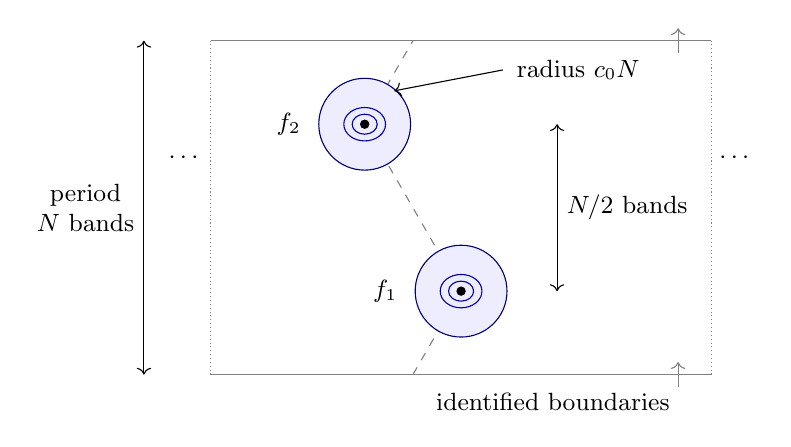
\begin{tikzpicture}[scale=1.06,every node/.style={font=\small}]
 \draw[gray] (-3,0)--(3,0) (-3,4)--(3,4);
 \draw[gray,densely dotted] (-3,0)--(-3,4) (3,0)--(3,4);
 \node at (-3.3,2.6) {$\cdots$};
 \node at (3.3,2.6) {$\cdots$};
 \draw[gray,dashed] (-.577,0)--(0,1)--(-1.155,3)--(-.577,4);
 \foreach \xx/\yy in {0/1,-1.155/3} {
   \fill[blue!7] (\xx,\yy) circle (.55);
   \draw[blue!45!black] (\xx,\yy) circle (.55);
   \draw[blue!65!black] (\xx,\yy) ellipse (.25 and .20);
   \draw[blue!65!black] (\xx,\yy) ellipse (.15 and .12);
   \fill (\xx,\yy) circle (1.6pt);
 }
 \node[left] at (-.65,1) {$f_1$};
 \node[left] at (-1.805,3) {$f_2$};
 \draw[<->] (1.15,1)--(1.15,3)
   node[midway,right] {$N/2$ bands};
 \draw[<->] (-3.8,0)--(-3.8,4)
   node[midway,left,align=center] {period\\$N$ bands};
 \draw[->,gray] (2.6,-.15)--(2.6,.15);
 \draw[->,gray] (2.6,3.85)--(2.6,4.15);
 \node[below] at (1.1,-.1) {identified boundaries};
 \draw[->] (.5,3.65)--(-.8,3.4);
 \node[right] at (.55,3.65) {radius $c_0N$};
\end{tikzpicture}
\caption{A schematic fundamental band of the cylinder, with the lattice
suppressed. The dashed column cut follows the two balanced row blocks;
its marked seams have displacement $-N/4+iN\sqrt3/4$ and are separated
vertically by half the period. For small fixed $c_0$,
their radius-$c_0N$ neighborhoods are disjoint and embed isometrically
in the plane. After essential and larger polygons are deleted at bounded
cost, each remaining polygon belongs to a nest in one of these two
neighborhoods. The independent choices give the square of the planar
partition in \eqref{eq:05-cylinder-planar-comparison}.}
\label{fig:E-planar-comparison}
\end{figure}

\begin{proof}
The two cylinder markers have disjoint neighborhoods of radius
\(c_0N\), each isometric to its planar neighborhood, if \(c_0\) is
small enough: along the standard balanced column cut their displacement
is \(-N/4+iN\sqrt3/4\), and their vertical separation is half the
balanced period.
Figure~\ref{fig:E-planar-comparison} shows the two embedded neighborhoods.
Delete all separating essential polygons, using
Proposition~\ref{prop:05-winding-suppression}, and all contractible
polygons of lifted diameter greater than \(c_0N\), using
Lemma~\ref{lem:05-macroscopic-removal} at both markers. The product of
the deletion costs is uniformly bounded.

Every remaining polygon is contractible and encloses exactly one marker
in its disk. A planar simple curve of diameter at most \(r\) enclosing a
point lies in the radius-\(r\) neighborhood of that point: the point is
in the curve's convex hull, so its distance to each curve point is at
most the curve's diameter. Hence each remaining polygon lies in its
marker's embedded neighborhood. Conversely, a planar nest counted by
\(P_\chi(c_0N)\) projects into that neighborhood and separates the
cylinder markers. The neighborhoods are disjoint, so the two nests can
be chosen independently. Retaining just these configurations gives the
lower bound, and the preceding deletion gives the upper bound in
\eqref{eq:05-cylinder-planar-comparison}.

For each fixed \(\chi>0\), Theorem~\ref{thm:04-cylinder-exponent} gives
\(Z_N(\chi)=N^{\tau(\chi)+o(1)}\) along even \(N\). Taking logarithms
in the comparison yields
\(P_\chi(c_0N)=N^{\tau(\chi)/2+o(1)}\). Monotonicity in the radius and
bracketing an arbitrary radius between consecutive admissible values
prove \eqref{eq:05-planar-all-fugacity}. At \(\chi=2\),
\(\tau(2)=1/6\), giving \eqref{eq:05-planar-nest-scaling}.
\end{proof}

\subsection{Nests around the middle of a strip}

Let \(S_k\) be the partition sum of nests around a face center \(f\)
on the middle line of the strip \(\mathcal S_{2k}\) of \(2k\) triangular
bands. Thus \(S_k\) sums the finite vertex-disjoint nests enclosing \(f\),
with weight \(\prod_P2\rho^{|P|}\), including the empty nest.

\begin{corollary}[Middle-face nesting]\label{E:strip-nesting}
As \(k\longrightarrow\infty\),
\begin{equation}
 S_k=k^{1/12+o(1)}.
 \label{eq:C-nest}
\end{equation}
\end{corollary}
\begin{proof}
Choose a fixed \(c_0>0\) so small that every nest enclosing \(f\),
with each polygon of diameter at most \(c_0k\), fits inside the strip. By
Lemma~\ref{lem:05-macroscopic-removal}, deleting all larger polygons
has a bounded cost. Therefore
\[
 P_2(c_0k)\le S_k\le C P_2(c_0k).
\]
Apply Theorem~\ref{thm:05-nest-normalization}.
\end{proof}

\subsection{A positive comparison between length and nests}

We use the boundary winding identity to count visits to one internal
edge by summing over all ordered boundary sources and endpoints. This
local comparison will convert the nesting exponent into a length
exponent. Recall \(t=3/8\), \(c=\cos(3\pi/8)\), and \(d=1/\sqrt2\).

For a finite simply connected union $D$ of triangular tiles with simple
polygonal boundary and a boundary port $a$, the boundary identity of \cite[Lemma~2.1]{StripCompanion} is
\begin{equation}\label{eq:E-boundary-input}
 \sum_{b\in\partial D}\sum_{\gamma:a\to b}
       \rho^{n(\gamma)}e^{itW(\gamma)}=1,
\end{equation}
where $W$ measures signed turning from the inward initial direction to
the outward final direction. Its local rule sends the current weight
into the two new continuations with multipliers
$\rho e^{i\lambda}$ and $\rho e^{-i\lambda}$; their sum is one.
At a first self-collision, reversing the closing cycle gives the
canceling winding increments $\pm4\pi/3$. In a convex domain every
boundary-to-boundary path satisfies $|W|\le\pi$, and therefore
$c\le\cos(tW)\le1$. These conventions also specify the modified
interior-source calculation below.


For a finite convex union $D$ of triangular tiles and an internal
honeycomb mid-edge $p$, define
\[
 L_p(D)=\sum_{a,b\in\partial D}\ \sum_{\gamma:a\to b}
 \rho^{n(\gamma)}\cos(tW(\gamma))\,
 \mathbf1_{\{p\in\gamma\}}.
\]
The boundary ports are ordered, and $W(\gamma)$ is the total signed
turning from the initial inward direction to the final outward direction.
Convexity gives $c\le\cos(tW(\gamma))\le1$.
For a point $r$ not on a polygon, let $\mathcal Z_r(D)$ be the sum over
finite sets of pairwise vertex-disjoint simple polygons, all strictly
enclosing $r$, with weight $\prod_\ell 2\rho^{|\ell|}$; the empty set
has weight one. The same definition applies when $r$ is a mid-edge,
excluding polygons through that mid-edge.

\begin{lemma}[Length and polygon nests]\label{lem:02-length-nests}\label{E:length-nest}
Let $f_1,f_2$ be the two honeycomb face centers adjacent to $p$. Then
\[
 d\bigl(\mathcal Z_{f_1}(D)+\mathcal Z_{f_2}(D)\bigr)
 \le L_p(D)\le
 \mathcal Z_{f_1}(D)+\mathcal Z_{f_2}(D).
\]
The inequalities also hold, with finite quantities, in every homogeneous
infinite strip of fixed positive height.
\end{lemma}
\begin{proof}
Cut the edge at $p$ into two stopping outlets. For a boundary source
$a$, the winding splitting identity still has total one: every collision
stem approaches its closing cycle from outside, so the two orientations
cancel. Subtract this identity from the one without the cut. The total
winding weight of paths visiting $p$ equals that of paths from $a$
stopping at the cut. Reversing these paths and taking real parts gives
$L_p(D)=F_+(D)+F_-(D)$, where $F_\sigma$ is the real winding-weighted
sum of paths from the specified side $p^\sigma$ to the exterior. The
initial direction points into the neighboring vertex on that side.

Apply the same splitting procedure from this interior source, retaining
all stopping possibilities. A return to the other side of the cut traces
a polygon $\ell'$ through $p$. For a fixed initial side it is counted
once and has turning $\pm2\pi$, hence real factor
$\cos(2\pi t)=-d$. A collision with a polygon not enclosing $p$
cancels with its reversed orientation. If its polygon $\ell$ strictly
encloses $p$, the stem approaches from inside. The closing turn of the
counterclockwise polygon at the collision vertex is $-\pi/3$, whereas
the turn from the stem into that orientation is $+\pi/3$. The added
winding is therefore $8\pi/3$, or $-8\pi/3$ for the other orientation.
Both have factor $\exp(\pm it8\pi/3)=-1$.

For a fixed enclosing $\ell$, sum the stems in its interior, excluding
its vertices. This is exactly the corresponding $F_\sigma$ for the
smaller domain: the stem stops at the mid-edge before its aimed-at
vertex, whose weight belongs to $\ell$. If its initial direction already
points at an excluded vertex, this stem sum is one. No further inner
polygon is then possible. Write \(D_\ell\) for the domain strictly inside an enclosing polygon
\(\ell\), with its vertices excluded and with stopping outlets on the
incident half-edges. Conservation of the initial mass, followed by the
collision classification above, gives the recurrence
\[
 F_\sigma(D)=1+d\sum_{\ell'\ni p}\rho^{|\ell'|}
       +2\sum_{\ell\text{ enclosing }p}\rho^{|\ell|}F_\sigma(D_\ell).
\]
The factor two in the last sum comes from the two orientations of the
enclosing polygon, each with real factor \(-1\) on the stopped side
of the conservation identity. The initial-source convention just
specified gives \(F_\sigma(D_\ell)=1\) if its first vertex is excluded.

Iterate this recurrence, choosing an outermost enclosing polygon first
and then polygons strictly inside it. Every nested family is obtained
once in this order. The iteration terminates either with the constant
term one or with a polygon through \(p\); such a polygon must be the
innermost selected cycle: \(p\) lies on its boundary, so no disjoint
cycle strictly inside its bounded disk can enclose \(p\). Every enclosing cycle removes vertices,
so the iteration is finite. It gives, for either sign,
\[
 F_\sigma(D)=\mathcal Z_p(D)+d\sum_{\ell'\ni p}
       \rho^{|\ell'|}\mathcal Z_{\mathrm{around}}(\ell'),
\]
where $\mathcal Z_{\mathrm{around}}(\ell')$ sums the disjoint outer
polygons surrounding $\ell'$, with fugacity two per polygon. This
recursion remains valid if the opposite neighbor of $p$ is excluded;
in that case there is no return to the cut.

A polygon enclosing exactly one of $f_1,f_2$ uses their separating
edge. There can be at most one such polygon in a disjoint nest, and it
is the innermost polygon of that nest: any smaller polygon around the
same face would also have to use that edge. Consequently
\[
 \mathcal Z_{f_1}(D)+\mathcal Z_{f_2}(D)
 =2\mathcal Z_p(D)+2\sum_{\ell'\ni p}
       \rho^{|\ell'|}\mathcal Z_{\mathrm{around}}(\ell').
\]
Together with the preceding expression for $F_++F_-$ and $0<d<1$,
this proves the finite-domain claim.

Exhaust an infinite strip by parallelograms. The top/bottom path sums
and the nesting sums increase. The terms with a distant side-wall
endpoint tend to zero. To justify the latter assertion, split a path
at $p$ and discard avoidance between its arms. Keep a fixed group of
columns containing $p$. On either side, the vacuum transfer supplies
a uniformly bounded half-state. A top/bottom endpoint is bounded by
the sum over its source column followed by one-defect propagation to
the fixed columns; this sum converges by the fixed-height transfer
decay. A side-wall endpoint contributes a decaying one-defect power,
with only finitely many wall ports. Thus each arm is uniformly summable
and its side-wall part tends to zero. The upper bound on $L_p$ obtained
in this way and the lower finite-domain inequality also prove finiteness
of the limiting nesting sums.
\end{proof}


\subsection{Raw and conditioned first-length estimates}

We now keep a single bottom boundary port \(a\) fixed. Let
\(\mathcal P_N(a)\) be the self-avoiding port paths in the open
\(N\)-band strip from \(a\) to either boundary, with no other boundary
visit. These are the bottom arches and the bridges. Their terminal
ports are summed over their actual lattice positions; there is no
additional translation sum. Write
\[
 \mathcal M_N(a)=\sum_{\gamma\in\mathcal P_N(a)}
                  \rho^{n(\gamma)}n(\gamma),
\]
where \(n(\gamma)\) counts visited honeycomb vertices. This is an
unnormalized first-length mass.

\begin{proposition}[Raw first-length mass]\label{E:raw-first-moment}
There is a constant \(C\), independent of the boundary source and
\(N\ge1\), such that
\begin{equation}
 \mathcal M_N(a)\le C(1+NS_{N+1})
                      \le N^{13/12+o(1)}
 \qquad(N\longrightarrow\infty).
 \label{eq:05-raw-first-moment}
\end{equation}
\end{proposition}
\begin{proof}
Sum \(L_p(\mathcal S_N)\) over one representative of each internal
mid-edge orbit under integer horizontal translation. For each summand, translate its source port to the fixed representative
of its boundary orbit. The marked internal edge then runs through all
visits of the translated path. This is a bijection between the two sets
of path--edge pairs, preserving both length and winding; hence translation
invariance turns the sum into the winding-weighted number of internal
edge visits for paths from the chosen source representatives.
There is one bottom-port orbit and one top-port orbit, whose source
totals agree by a half-turn. Thus, if \(\mathcal E_N\) is the chosen
set of internal mid-edge representatives, the orbit-count identity is
\[
 \sum_{p\in\mathcal E_N}L_p(\mathcal S_N)
 =2\sum_{\gamma\in\mathcal P_N(a)}
       \rho^{n(\gamma)}(n(\gamma)-1)\cos(tW(\gamma)).
\]
A path with \(n\) vertices has \(n-1\) internal mid-edge visits, and
its winding cosine is between \(c\) and one. There are \(O(N)\)
internal edge orbits. These positive sums may be rearranged by monotone
convergence.

Every face-center nesting mass in the strip is at most \(S_{N+1}\):
embed the strip in a \(2(N+1)\)-band strip whose middle line contains
the chosen face center. Lemma~\ref{lem:02-length-nests} now bounds the
sum of internal edge visits by \(CNS_{N+1}\). To replace \(n-1\) by
\(n\), add the boundary partition mass
\(\mathcal A_N+\mathcal B_N\le 1/c\), using the strip identity
\(c\mathcal A_N+\mathcal B_N=1\). This proves the first inequality;
Corollary~\ref{E:strip-nesting} proves its asymptotic form.
\end{proof}

\begin{proposition}[Length conditional on reaching macroscopic height]
\label{prop:02-length-reduction}
Give \(\mathcal P_N(a)\) its normalized critical weights. Conditional
on the path reaching the top boundary of the bottom
\(\lfloor N/4\rfloor\) bands, its
expected number of visited vertices is \(N^{4/3+o(1)}\).
\end{proposition}
\begin{proof}
Put \(k=\lfloor N/4\rfloor\), and take \(N\) large enough that
\(k\ge1\). A path is confined to the bottom \(k\)-band strip exactly
when it stays below its top line: crossing that line uses a port between
the two adjacent bands. Thus the conditioning event consists of all
bridges and precisely the bottom arches not counted by \(\mathcal A_k\).
Its unnormalized mass is
\[
 q_N=\mathcal B_N+\mathcal A_N-\mathcal A_k
     =\mathcal B_k/c-(1/c-1)\mathcal B_N
     \asymp N^{-1/4}.
\]
Indeed monotonicity gives
\(\mathcal B_k\le q_N\le\mathcal B_k/c\), and the strip theorem gives
\(\mathcal B_k\asymp N^{-1/4}\).

Restrict the orbit sum in the preceding proof to internal mid-edges
whose heights lie in the central third. For sufficiently large \(N\),
each adjacent face center is at distance at least \(N/3-O(1)>k\)
bands from either boundary. Its centered \(2k\)-band strip therefore
fits inside \(\mathcal S_N\), so its nesting mass is at least \(S_k\).
There are at least \(c_1N\) such internal edge orbits, and
Lemma~\ref{lem:02-length-nests} gives a lower bound \(c_2NS_k\) for
their total winding-weighted visit mass. Any bottom-source path counted
there reaches the top boundary of the bottom \(k\) bands; the rotated statement holds
for a top source. Since the winding cosine is at most one and the
number of counted visits is at most the path length, the unnormalized
first-length mass of the conditioning event is at least \(c_3NS_k\).
Its upper bound is \(\mathcal M_N(a)\). By
Corollary~\ref{E:strip-nesting} and
Proposition~\ref{E:raw-first-moment}, these bounds both have exponent
\(13/12\). Division by \(q_N\) gives
\(N^{13/12+1/4+o(1)}=N^{4/3+o(1)}\).
\end{proof}

\clearpage
\phantomsection
\addcontentsline{toc}{section}{References}
\begin{thebibliography}{99}
\bibitem{Cardy2006Annulus}
J.~Cardy. The $O(n)$ model on the annulus.
\emph{Journal of Statistical Physics} \textbf{125} (2006), 1--21.
\href{https://doi.org/10.1007/s10955-006-9186-8}{doi:10.1007/s10955-006-9186-8}.
\href{https://arxiv.org/abs/math-ph/0604043}{arXiv:math-ph/0604043}.

\bibitem{DiFrancescoZinnJustin2005}
P.~Di Francesco and P.~Zinn-Justin.
Around the Razumov--Stroganov conjecture: proof of a multi-parameter sum rule.
\emph{Electronic Journal of Combinatorics} \textbf{12} (2005), Research Paper~6.
\href{https://doi.org/10.37236/1903}{doi:10.37236/1903}.
\href{https://arxiv.org/abs/math-ph/0410061}{arXiv:math-ph/0410061}.

\bibitem{DiaconisEvans2001}
P.~Diaconis and S.~N.~Evans.
Linear functionals of eigenvalues of random matrices.
\emph{Transactions of the American Mathematical Society}
\textbf{353} (2001), 2615--2633.
\mbox{\href{https://doi.org/10.1090/S0002-9947-01-02800-8}{doi:10.1090/S0002-9947-01-02800-8}}.

\bibitem{DiaconisShahshahani1994}
P.~Diaconis and M.~Shahshahani.
On the eigenvalues of random matrices.
\emph{Journal of Applied Probability} \textbf{31A} (1994), 49--62.
\href{https://doi.org/10.1017/S0021900200106989}{doi:10.1017/S0021900200106989}.

\bibitem{DCS2012}
H.~Duminil-Copin and S.~Smirnov.
The connective constant of the honeycomb lattice equals $\sqrt{2+\sqrt2}$.
\emph{Annals of Mathematics} \textbf{175} (2012), 1653--1665.
\href{https://doi.org/10.4007/annals.2012.175.3.14}{doi:10.4007/annals.2012.175.3.14}.

\bibitem{DuminilCopinHammond2013}
H.~Duminil-Copin and A.~Hammond. Self-avoiding walk is sub-ballistic.
\emph{Communications in Mathematical Physics} \textbf{324} (2013), 401--423.
\href{https://doi.org/10.1007/s00220-013-1811-1}{doi:10.1007/s00220-013-1811-1}.
\href{https://arxiv.org/abs/1205.0401}{arXiv:1205.0401}.

\bibitem{GamsaCardy2006}
A.~Gamsa and J.~Cardy.
Correlation functions of twist operators applied to single self-avoiding loops.
\emph{Journal of Physics A: Mathematical and General}
\textbf{39} (2006), 12983--13003.
\href{https://doi.org/10.1088/0305-4470/39/41/S12}{doi:10.1088/0305-4470/39/41/S12}.
\href{https://arxiv.org/abs/math-ph/0606065}{arXiv:math-ph/0606065}.

\bibitem{GarbaliNienhuis2017Ground}
A.~Garbali and B.~Nienhuis.
The dilute Temperley--Lieb $O(n=1)$ loop model on a semi infinite strip:
the ground state.
\emph{Journal of Statistical Mechanics: Theory and Experiment} (2017), 043108.
\href{https://doi.org/10.1088/1742-5468/aa6a30}{doi:10.1088/1742-5468/aa6a30}.
\href{https://arxiv.org/abs/1411.7020}{arXiv:1411.7020}.

\bibitem{GarbaliNienhuis2017Sum}
A.~Garbali and B.~Nienhuis.
The dilute Temperley--Lieb $O(n=1)$ loop model on a semi infinite strip:
the sum rule.
\emph{Journal of Statistical Mechanics: Theory and Experiment} (2017), 053102.
\href{https://doi.org/10.1088/1742-5468/aa6bc3}{doi:10.1088/1742-5468/aa6bc3}.
\href{https://arxiv.org/abs/1411.7160}{arXiv:1411.7160}.

\bibitem{GM2019}
A.~Glazman and I.~Manolescu.
Self-avoiding walk on $\mathbb Z^2$ with Yang--Baxter weights: universality of critical fugacity and 2-point function.
\emph{Annales de l'Institut Henri Poincar\'e, Probabilit\'es et Statistiques}
\textbf{56} (2020), 2281--2300.
\href{https://doi.org/10.1214/19-AIHP1024}{doi:10.1214/19-AIHP1024}.

\bibitem{Grafakos1997}
L.~Grafakos.
Best bounds for the Hilbert transform on $L^p(\mathbb R^1)$.
\emph{Mathematical Research Letters} \textbf{4} (1997), no.~4, 469--471.
\href{https://grafakos.missouri.edu/preprints/pichorides.pdf}{Author's text}.

\bibitem{GrafakosSavage2015}
L.~Grafakos and T.~Savage.
Best bounds for the Hilbert transform on $L^p(\mathbb R^1)$: A corrigendum.
\emph{Mathematical Research Letters} \textbf{22} (2015), no.~5, 1333--1335.
\href{https://grafakos.missouri.edu/preprints/grafakos-savage2.pdf}{Author's text}.

\bibitem{HammersleyWelsh1962}
J.~M.~Hammersley and D.~J.~A.~Welsh.
Further results on the rate of convergence to the connective constant
of the hypercubical lattice.
\emph{The Quarterly Journal of Mathematics} \textbf{13} (1962), 108--110.
\href{https://doi.org/10.1093/qmath/13.1.108}{doi:10.1093/qmath/13.1.108}.

\bibitem{IkhlefCardy2009}
Y.~Ikhlef and J.~Cardy.
Discretely holomorphic parafermions and integrable loop models.
\emph{Journal of Physics A: Mathematical and Theoretical}
\textbf{42} (2009), 102001.
\href{https://doi.org/10.1088/1751-8113/42/10/102001}{doi:10.1088/1751-8113/42/10/102001}.
\href{https://arxiv.org/abs/0810.5037}{arXiv:0810.5037}.

\bibitem{IshikawaOkadaTagawaZeng2006}
M.~Ishikawa, S.~Okada, H.~Tagawa and J.~Zeng.
Generalizations of Cauchy's determinant and Schur's Pfaffian.
\emph{Advances in Applied Mathematics} \textbf{36} (2006), 251--287.
\href{https://doi.org/10.1016/j.aam.2005.07.001}{doi:10.1016/j.aam.2005.07.001}.
\href{https://arxiv.org/abs/math/0411280}{arXiv:math/0411280}.

\bibitem{MadrasSlade1993}
N.~Madras and G.~Slade.
\emph{The Self-Avoiding Walk}.
Birkh\"auser, Boston, 1993.

\bibitem{DLMF18}
National Institute of Standards and Technology.
\emph{Digital Library of Mathematical Functions}, Chapter~18:
Orthogonal Polynomials.
\href{https://dlmf.nist.gov/18.18.E28}{Equation~18.18.28 (Mehler)};
\href{https://dlmf.nist.gov/18.2.E12}{equation~18.2.12 (Christoffel--Darboux)}.

\bibitem{Nienhuis1982}
B.~Nienhuis.
Exact critical point and critical exponents of $O(n)$ models in two dimensions.
\emph{Physical Review Letters} \textbf{49} (1982), 1062--1065.
\href{https://doi.org/10.1103/PhysRevLett.49.1062}{doi:10.1103/PhysRevLett.49.1062}.

\bibitem{StripCompanion}
OpenAI.
Critical strip-crossing mass on the honeycomb lattice.
OpenAI Math Release preprint
\href{https://github.com/openai/math/blob/main/preprints/Critical-strip-crossing-mass-on-the-honeycomb-lattice-September-26-2026/main.pdf}{OAI:Critical-strip-crossing-mass-on-the-honeycomb-lattice-September-26-2026},
2026.

\bibitem{Sarason2007}
D.~Sarason. Algebraic properties of truncated Toeplitz operators.
\emph{Operators and Matrices} \textbf{1} (2007), 491--526.
\href{https://doi.org/10.7153/oam-01-29}{doi:10.7153/oam-01-29}.

\bibitem{Simon2005Szego}
B.~Simon. The sharp form of the strong Szeg\H{o} theorem.
In \emph{Geometry, Spectral Theory, Groups, and Dynamics},
Contemporary Mathematics \textbf{387}, American Mathematical Society,
2005, 253--275.
\href{https://arxiv.org/abs/math/0402110}{arXiv:math/0402110}.

\bibitem{TracyWidom1998}
C.~A.~Tracy and H.~Widom.
Correlation functions, cluster functions and spacing distributions
for random matrices.
\emph{Journal of Statistical Physics} \textbf{92} (1998), 809--835.
\href{https://doi.org/10.1023/A:1023084324803}{doi:10.1023/A:1023084324803}.
\href{https://arxiv.org/abs/solv-int/9804004}{arXiv:solv-int/9804004}.

\bibitem{WienerHopf1931}
N.~Wiener and E.~Hopf.
\"Uber eine Klasse singul\"arer Integralgleichungen.
\emph{Sitzungsberichte der Preussischen Akademie der Wissenschaften,
Physikalisch-Mathematische Klasse} (1931), 696--706.

\bibitem{ZhouBatchelor1997}
Y.~K.~Zhou and M.~T.~Batchelor.
Critical behaviour of the dilute $O(n)$, Izergin--Korepin and dilute
$A_L$ face models: Bulk properties.
\emph{Nuclear Physics B} \textbf{485} (1997), 646--664.
\href{https://doi.org/10.1016/S0550-3213(96)00654-2}{doi:10.1016/S0550-3213(96)00654-2}.
\href{https://arxiv.org/abs/cond-mat/9611156}{arXiv:cond-mat/9611156}.
\end{thebibliography}

\end{document}
